% images.tex - All figure definitions for the MASK documentation

% Introduction figures
% PLACEMENT: Einführung.tex - Project introduction and mood setting
\begin{figure}[!htbp]
    \centering
    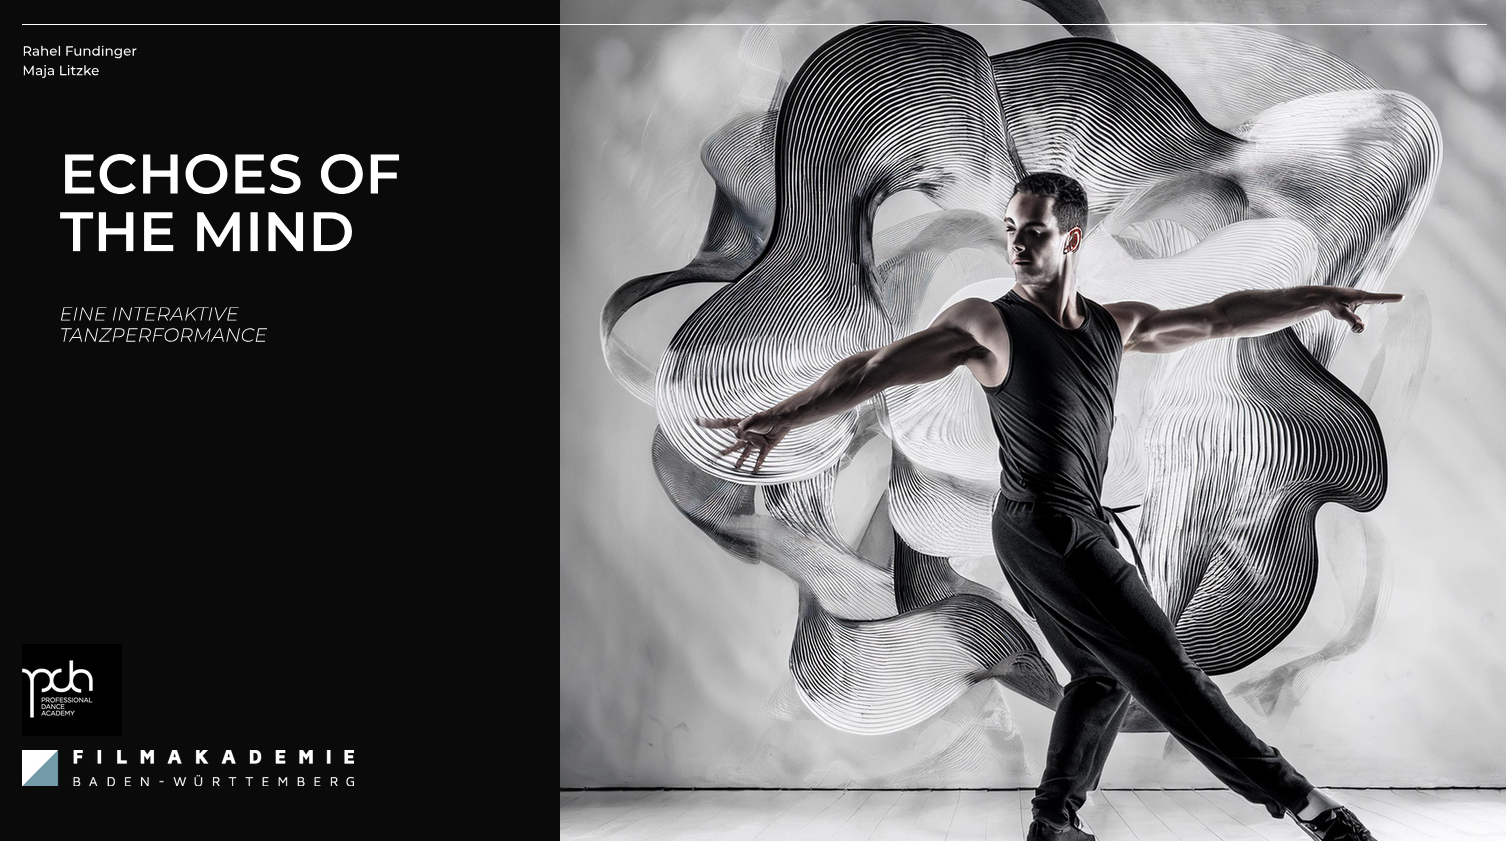
\includegraphics[width=0.6\textwidth,height=0.25\textheight,keepaspectratio]{images/EchoesOfTheMind_startbild.png}
    \caption{MoodBoard-Startbild des Projektes \glqq Echoes of the Mind\grqq{}}
    \label{fig:echoes_startbild}
\end{figure}

% PLACEMENT: Einführung.tex or problemstellung.tex - Artistic vision and project context
\begin{figure}[!htbp]
    \centering
    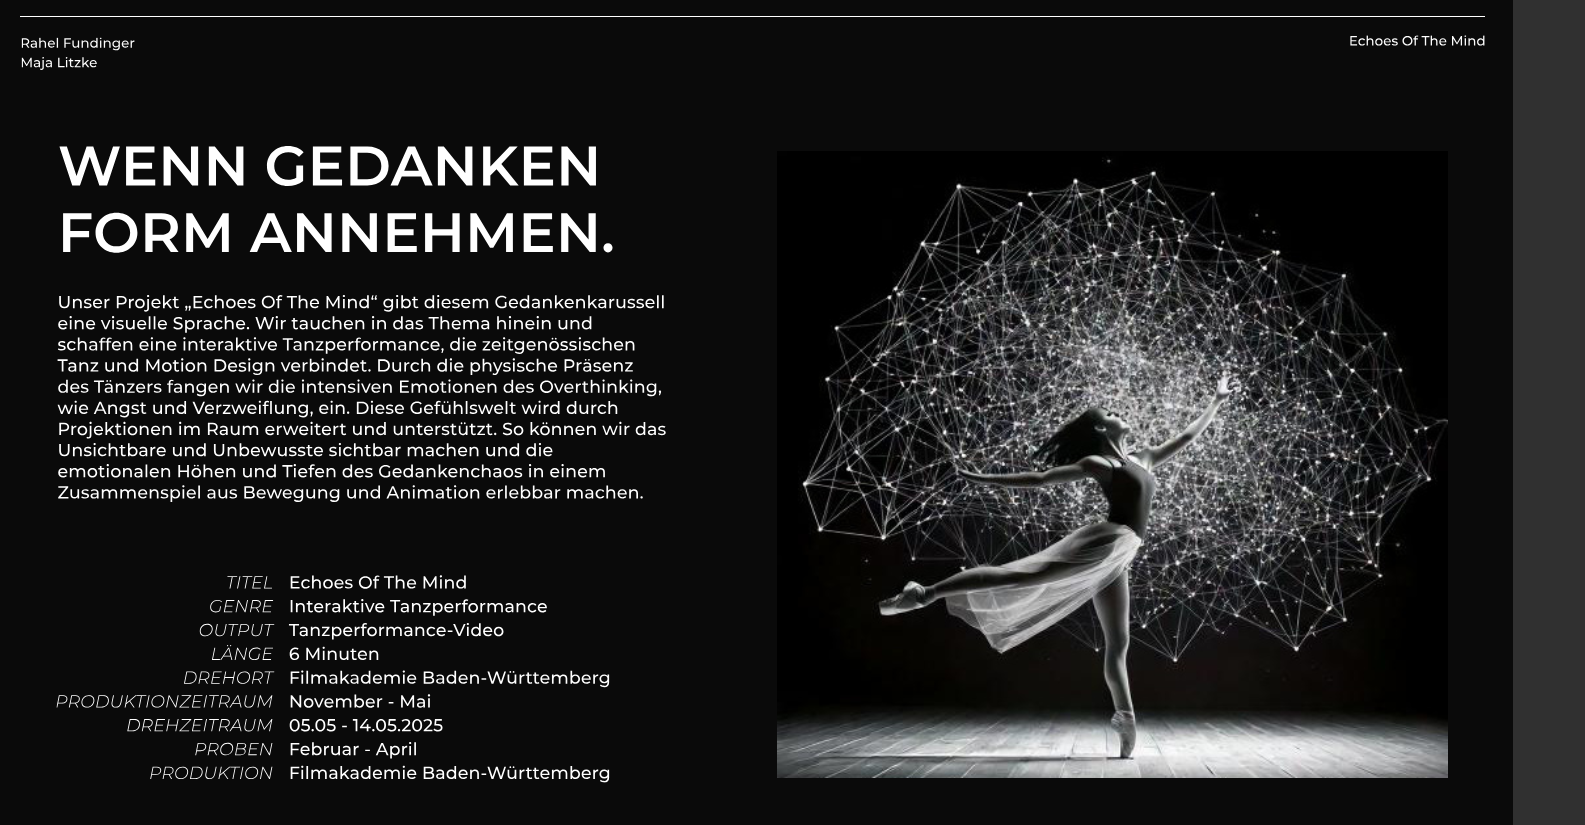
\includegraphics[width=0.6\textwidth,height=0.25\textheight,keepaspectratio]{images/EchoesOfTheMind_mood.png}
    \caption{K�nstlerische Vision: Emotionale Visualisierungskonzepte f�r \glqq Echoes of the Mind\grqq{}}
    \label{fig:echoes_mood}
\end{figure}

% Sprint 1 figures
% PLACEMENT: Systemarchitektur_und_Ergebnisse.tex - Core system architecture overview
\begin{figure}[!htbp]
    \centering
    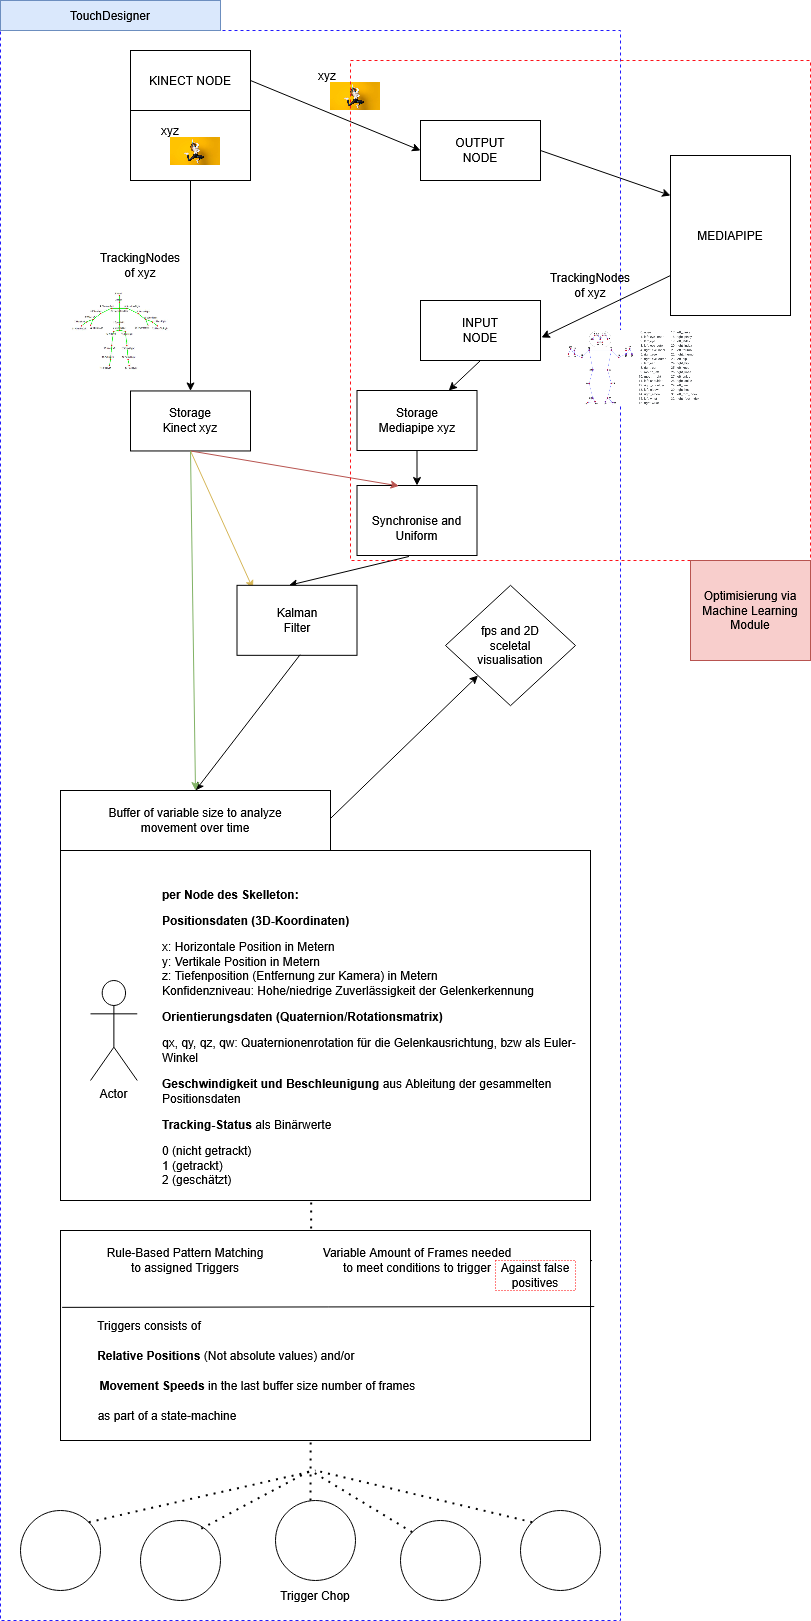
\includegraphics[width=0.6\textwidth,height=0.25\textheight,keepaspectratio]{images/MASK.png}
    \caption{M.A.S.K. Systemarchitektur: Analyse- und Triggerprozess}
    \label{fig:mask_architecture}
\end{figure}

% Sprint 2 figures
% PLACEMENT: stand_der_technik.tex or Systemarchitektur_und_Ergebnisse.tex - Technical foundation
\begin{figure}[!htbp]
    \centering
    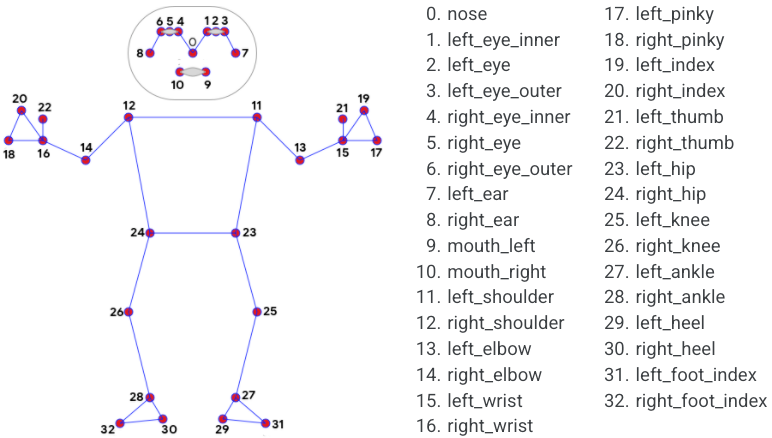
\includegraphics[width=0.6\textwidth,height=0.25\textheight,keepaspectratio]{images/mediapipeNODES.png}
    \caption{MediaPipe Skeleton-Node-Ausgabe mit Koordinaten und Confidence-Werten}
    \label{fig:mediapipe_nodes}
\end{figure}

% PLACEMENT: stand_der_technik.tex or Systemarchitektur_und_Ergebnisse.tex - Hardware specification
\begin{figure}[!htbp]
    \centering
    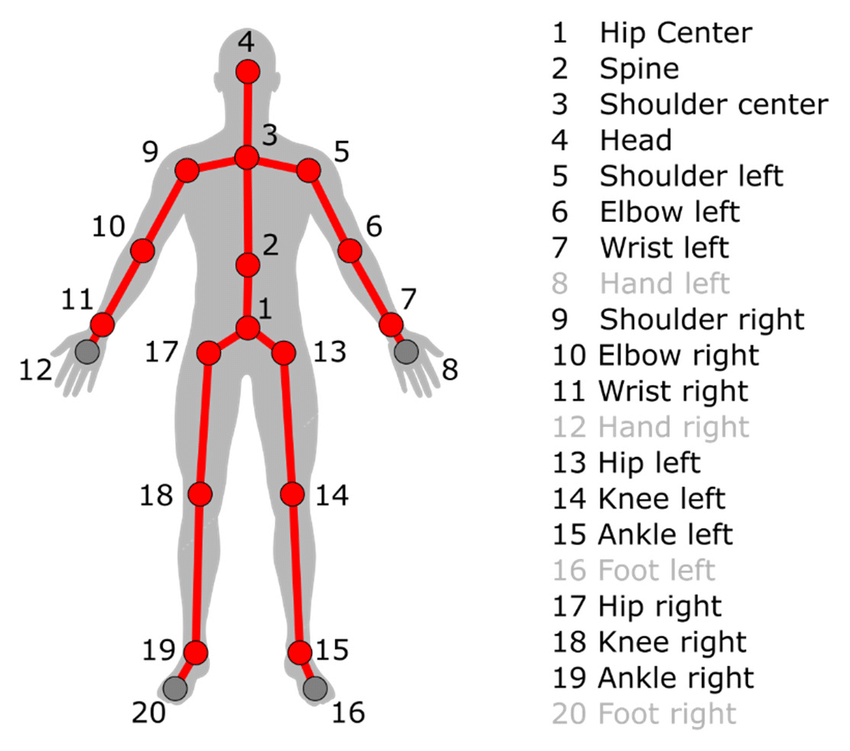
\includegraphics[width=0.6\textwidth,height=0.25\textheight,keepaspectratio]{images/kinect_nodes.png}
    \caption{Kinect V2 Skeleton-Visualisierung mit Node-Nummerierung}
    \label{fig:kinect_nodes}
\end{figure}

% PLACEMENT: Sprint2.tex or Entwicklungsprozess.tex - Development and testing phase
\begin{figure}[!htbp]
    \centering
    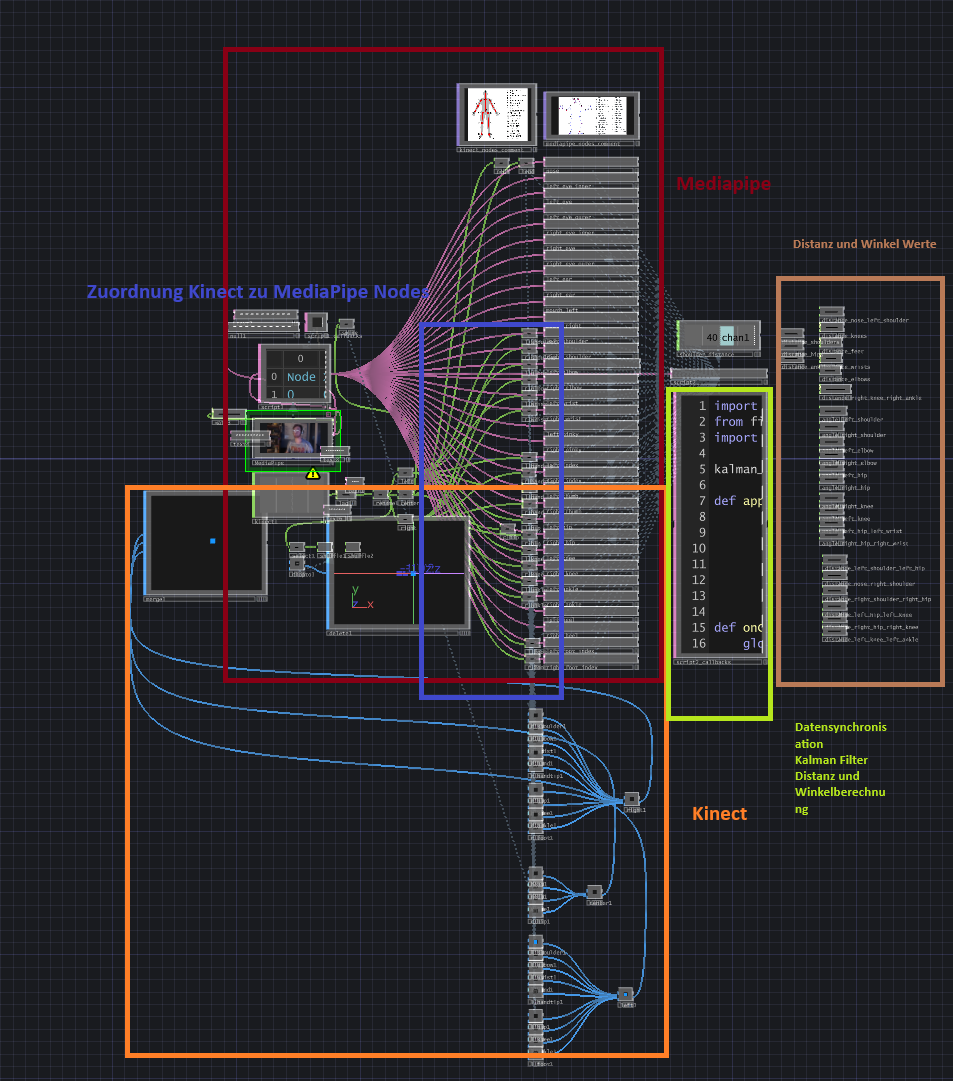
\includegraphics[width=0.6\textwidth,height=0.25\textheight,keepaspectratio]{images/docupictures/KinectMediaPipe_Testing.png}
    \caption{TouchDesigner-Interface f�r komparative Tracking-Tests}
    \label{fig:testing_interface}
\end{figure}

% Sprint 3 figures
% PLACEMENT: Sprint3.tex - Design concepts and scaling solutions
\begin{figure}[!htbp]
    \centering
    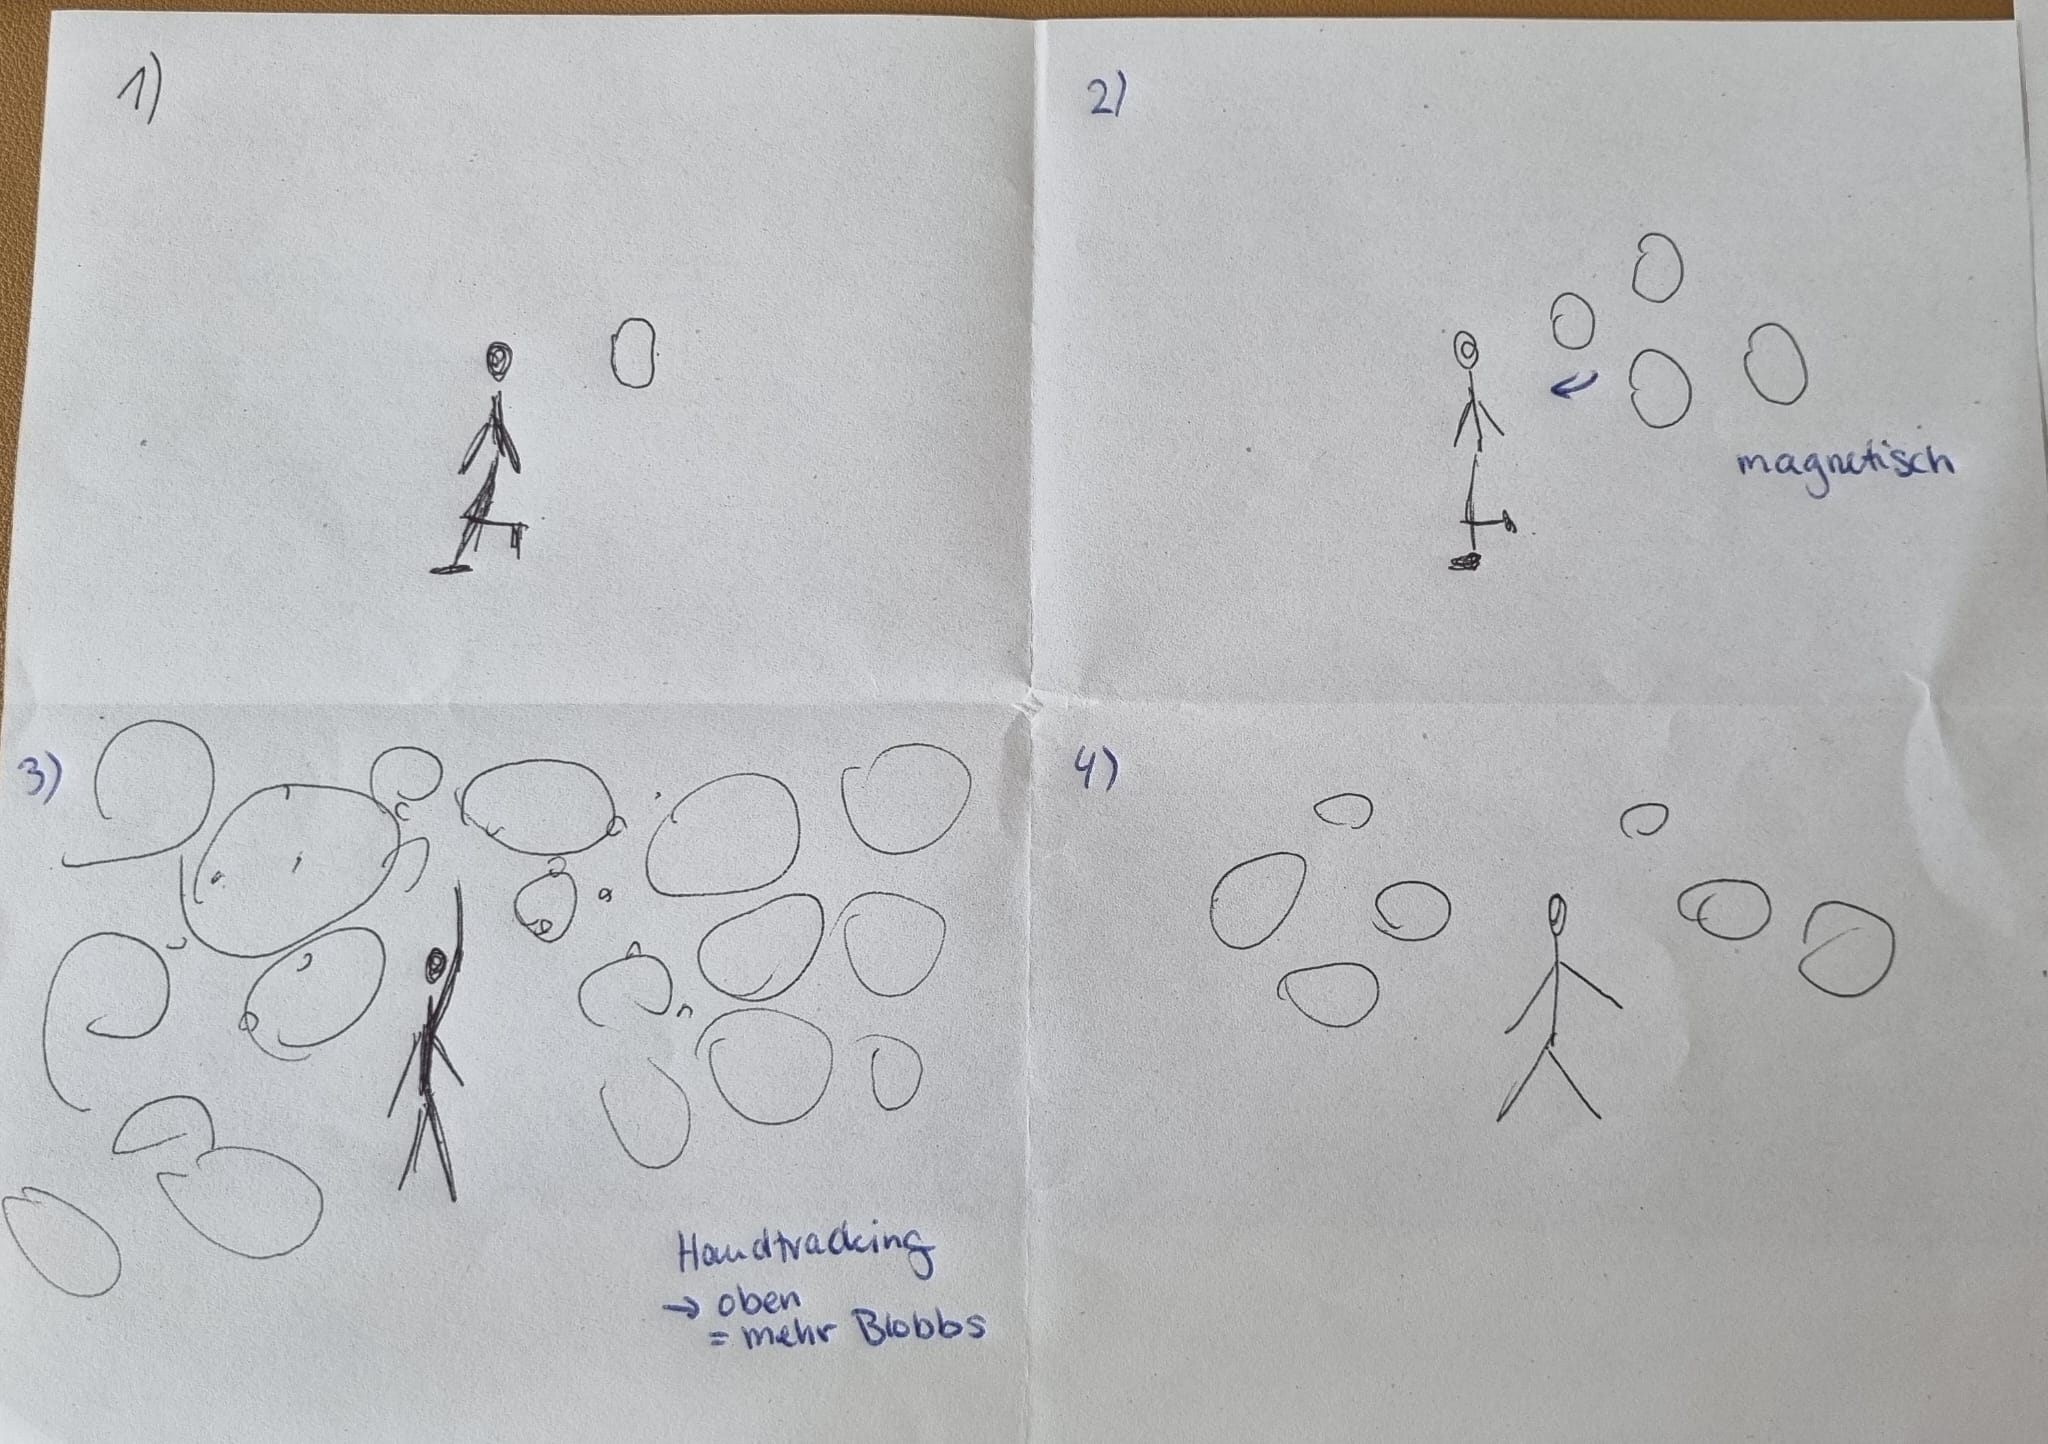
\includegraphics[width=0.6\textwidth,height=0.25\textheight,keepaspectratio]{images/Sprint3_1.jpg}
    \caption{Skalierungskonzept: Gr��enresponsive Visual-Transformation}
    \label{fig:scaling_concept}
\end{figure}

% PLACEMENT: Sprint3.tex - Spatial distribution concepts
\begin{figure}[!htbp]
    \centering
    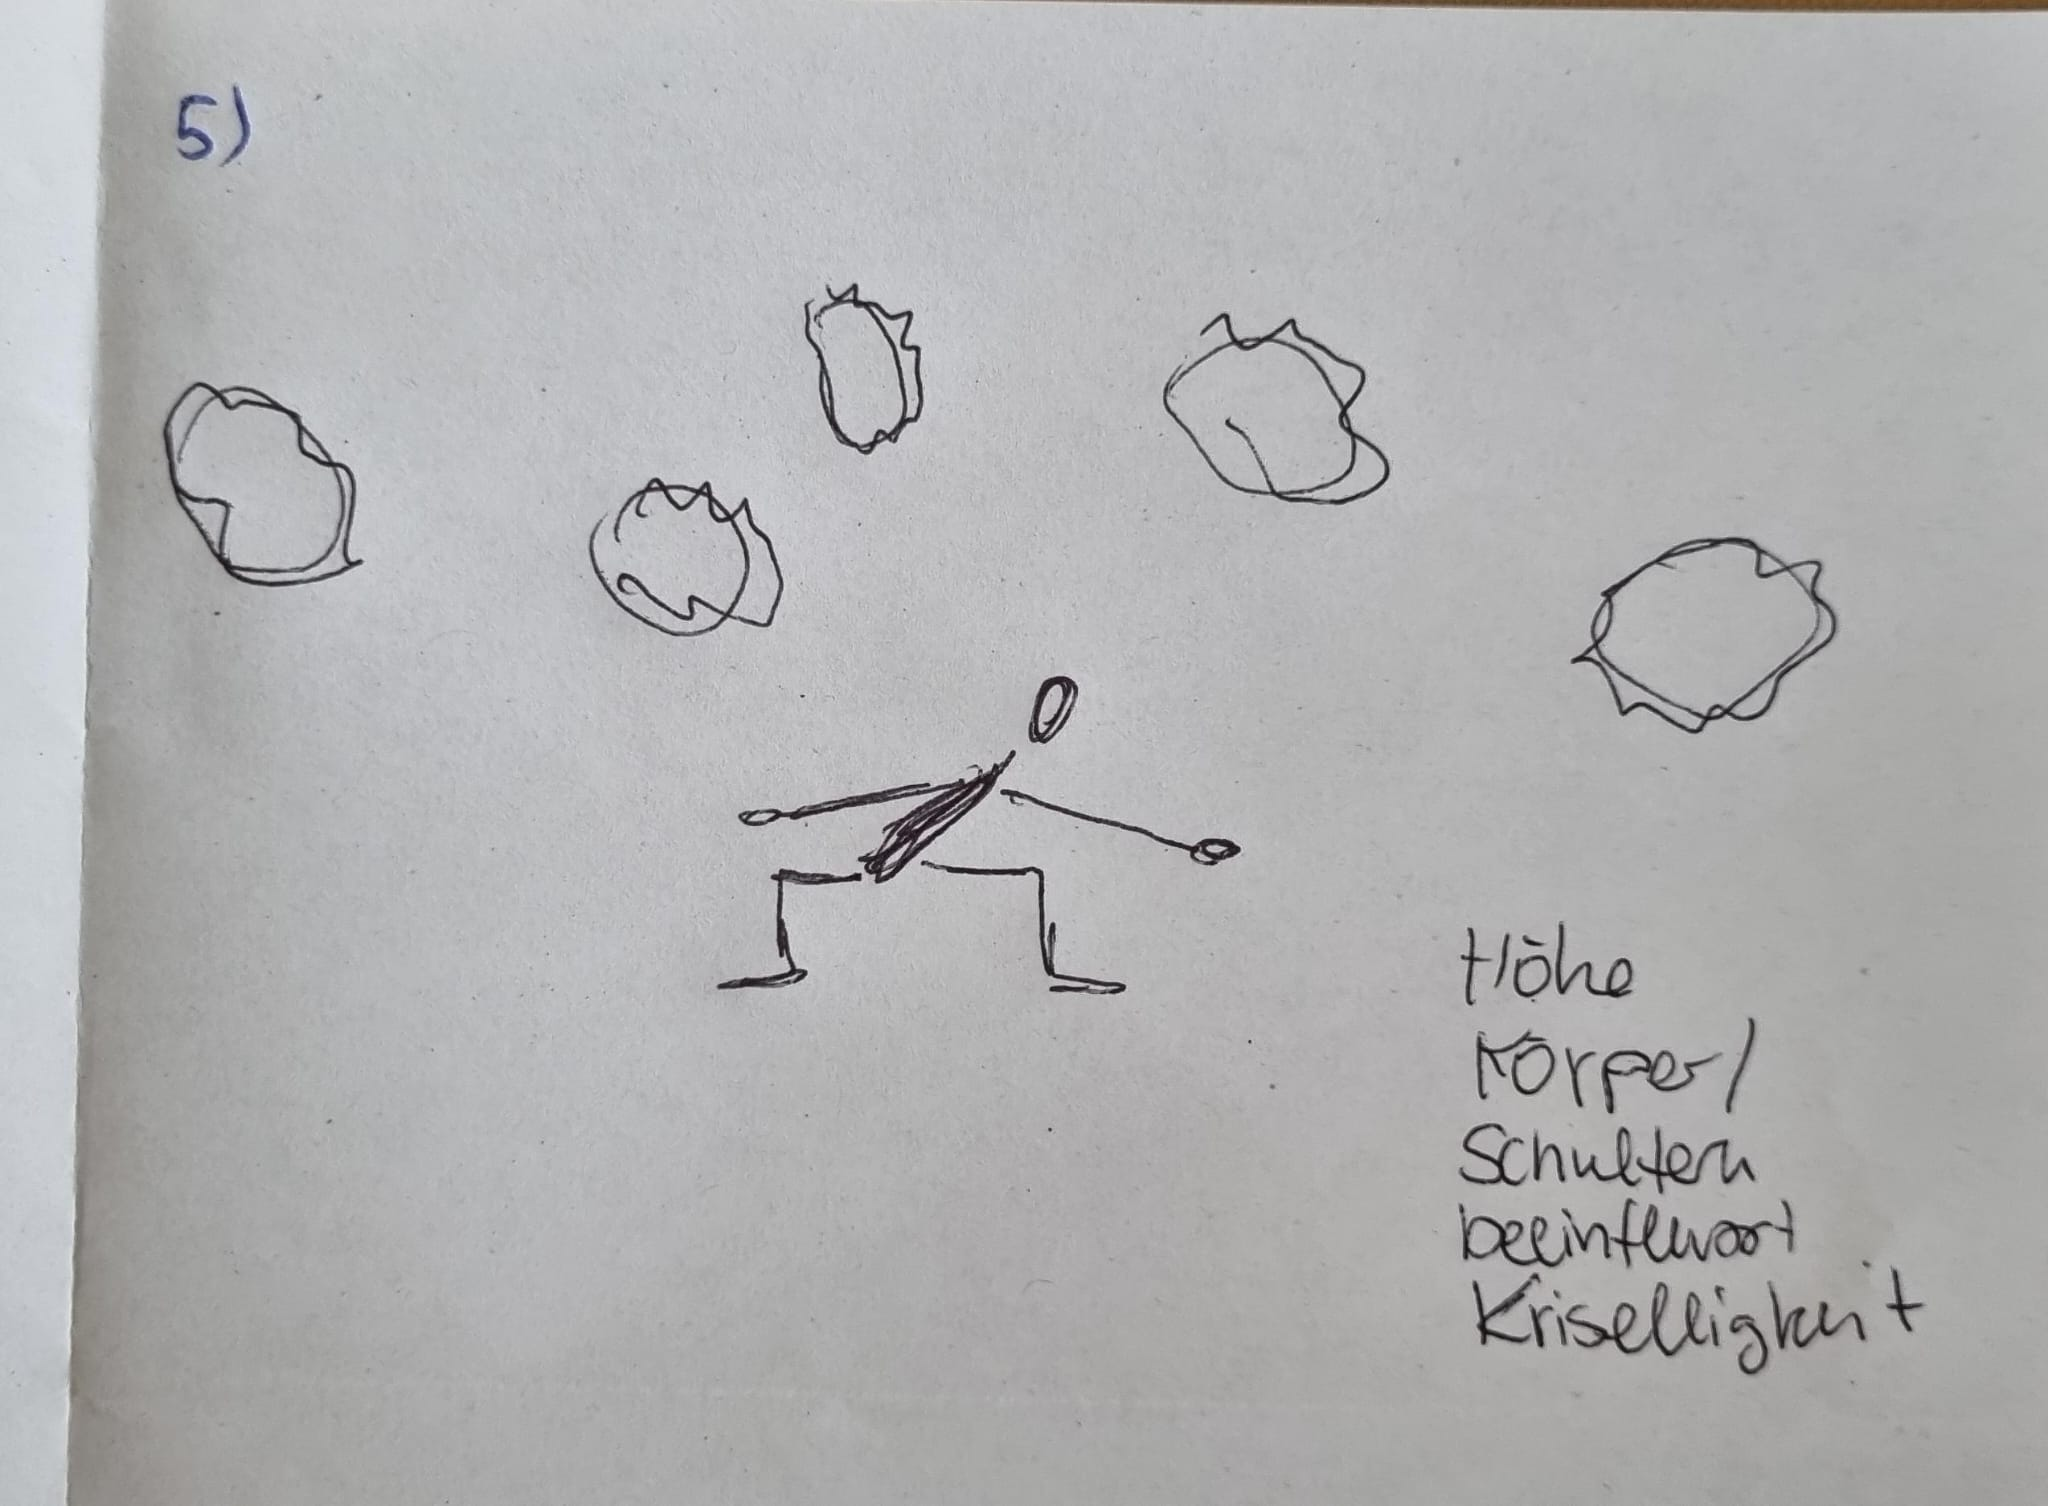
\includegraphics[width=0.6\textwidth,height=0.25\textheight,keepaspectratio]{images/Sprint3_2.jpg}
    \caption{R�umliche Verteilung: Externe Visual-Positionierung um Performer}
    \label{fig:external_positioning}
\end{figure}

% PLACEMENT: Sprint3.tex - Interaction design concepts
\begin{figure}[!htbp]
    \centering
    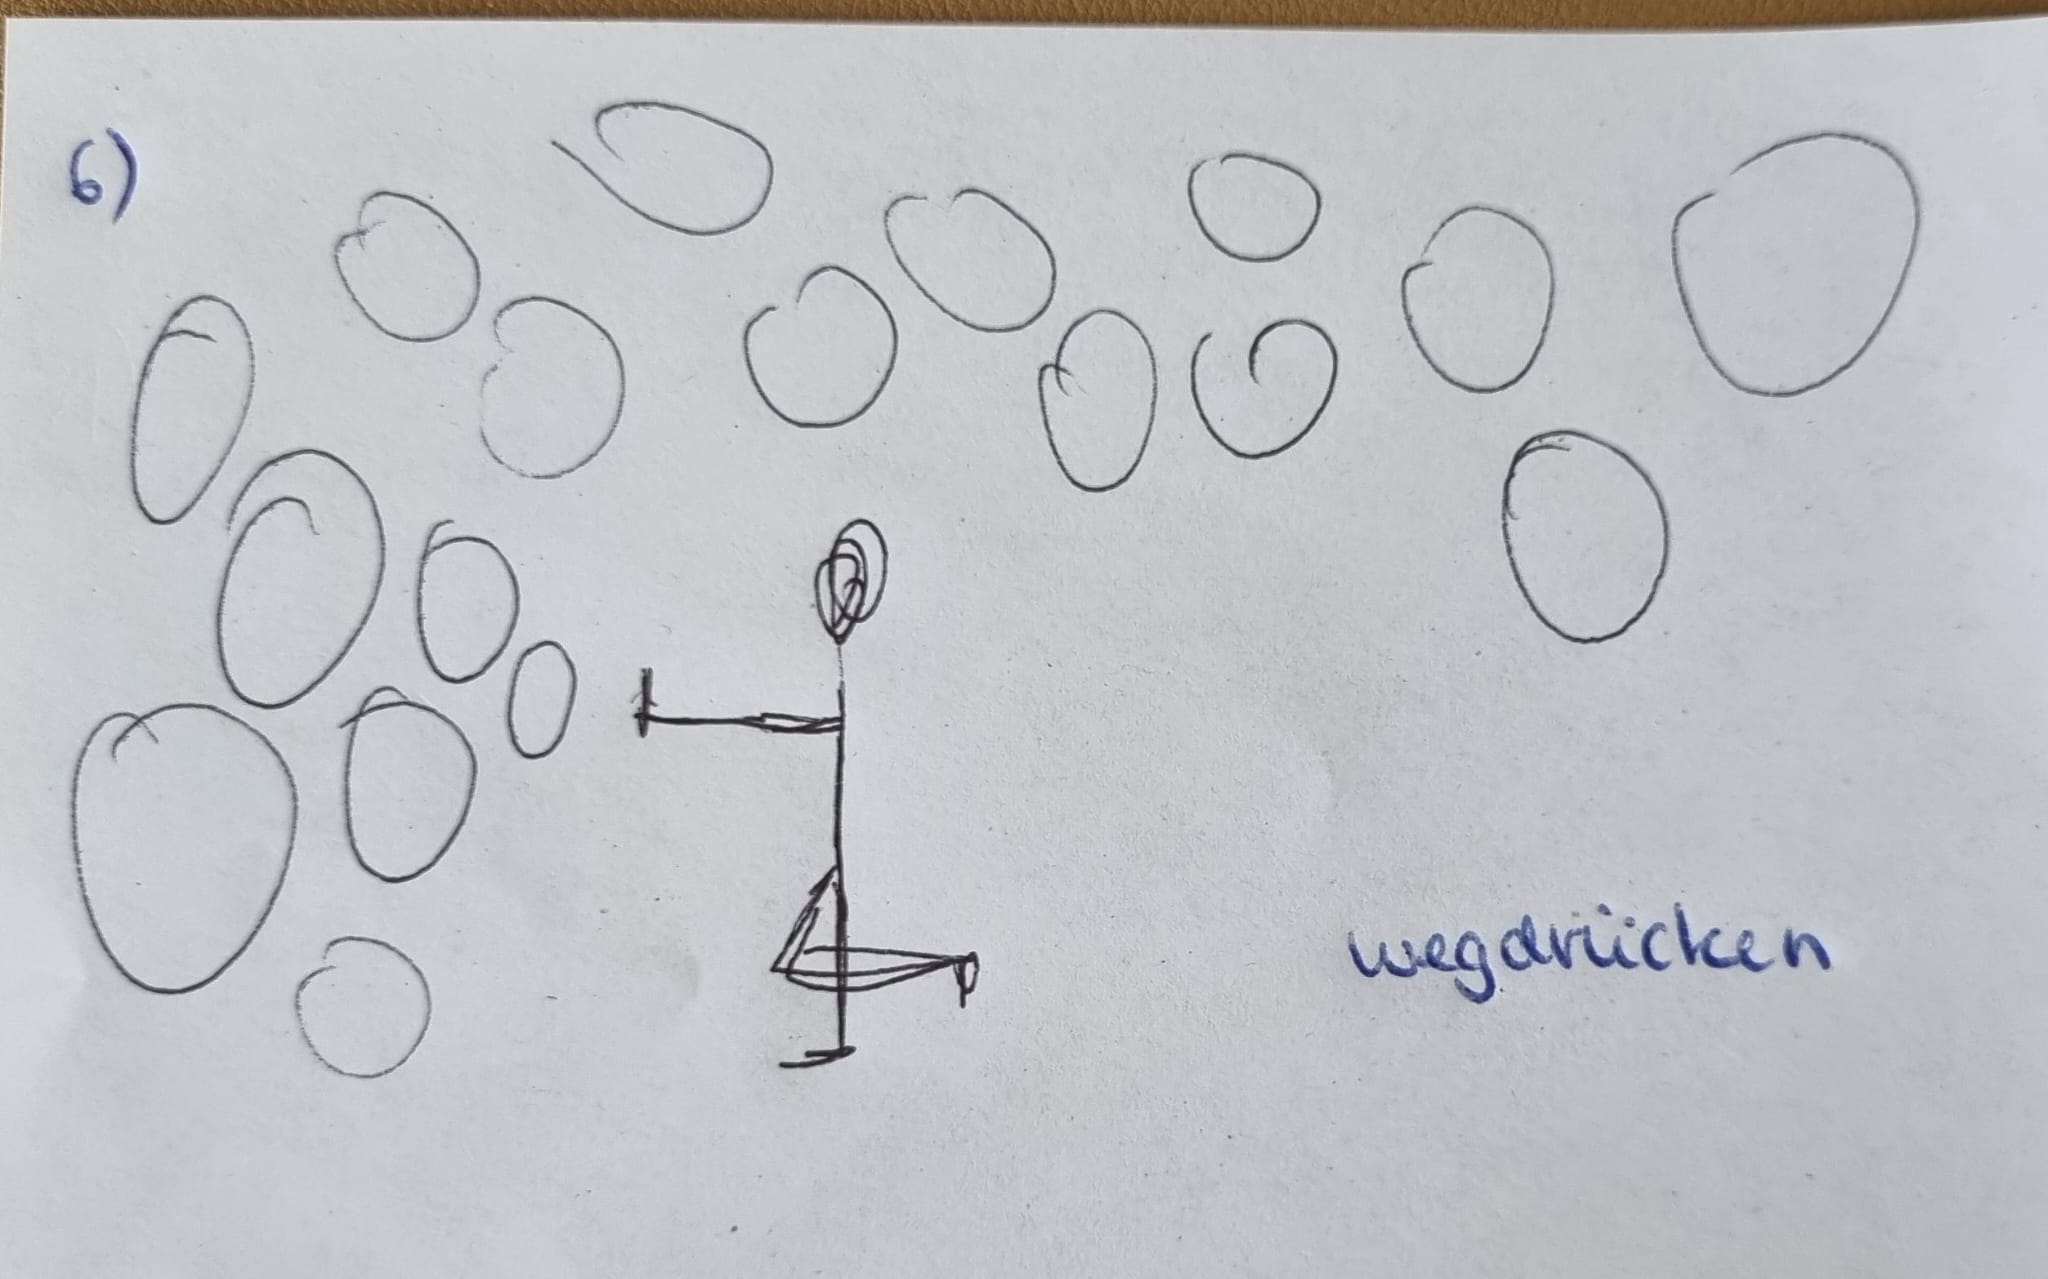
\includegraphics[width=0.6\textwidth,height=0.25\textheight,keepaspectratio]{images/Sprint3_3.jpg}
    \caption{Magnetische Interaktion: Dynamische Visual-Performer-Relation}
    \label{fig:magnetic_interaction}
\end{figure}

% PLACEMENT: Sprint3.tex - Movement-responsive system design
\begin{figure}[!htbp]
    \centering
    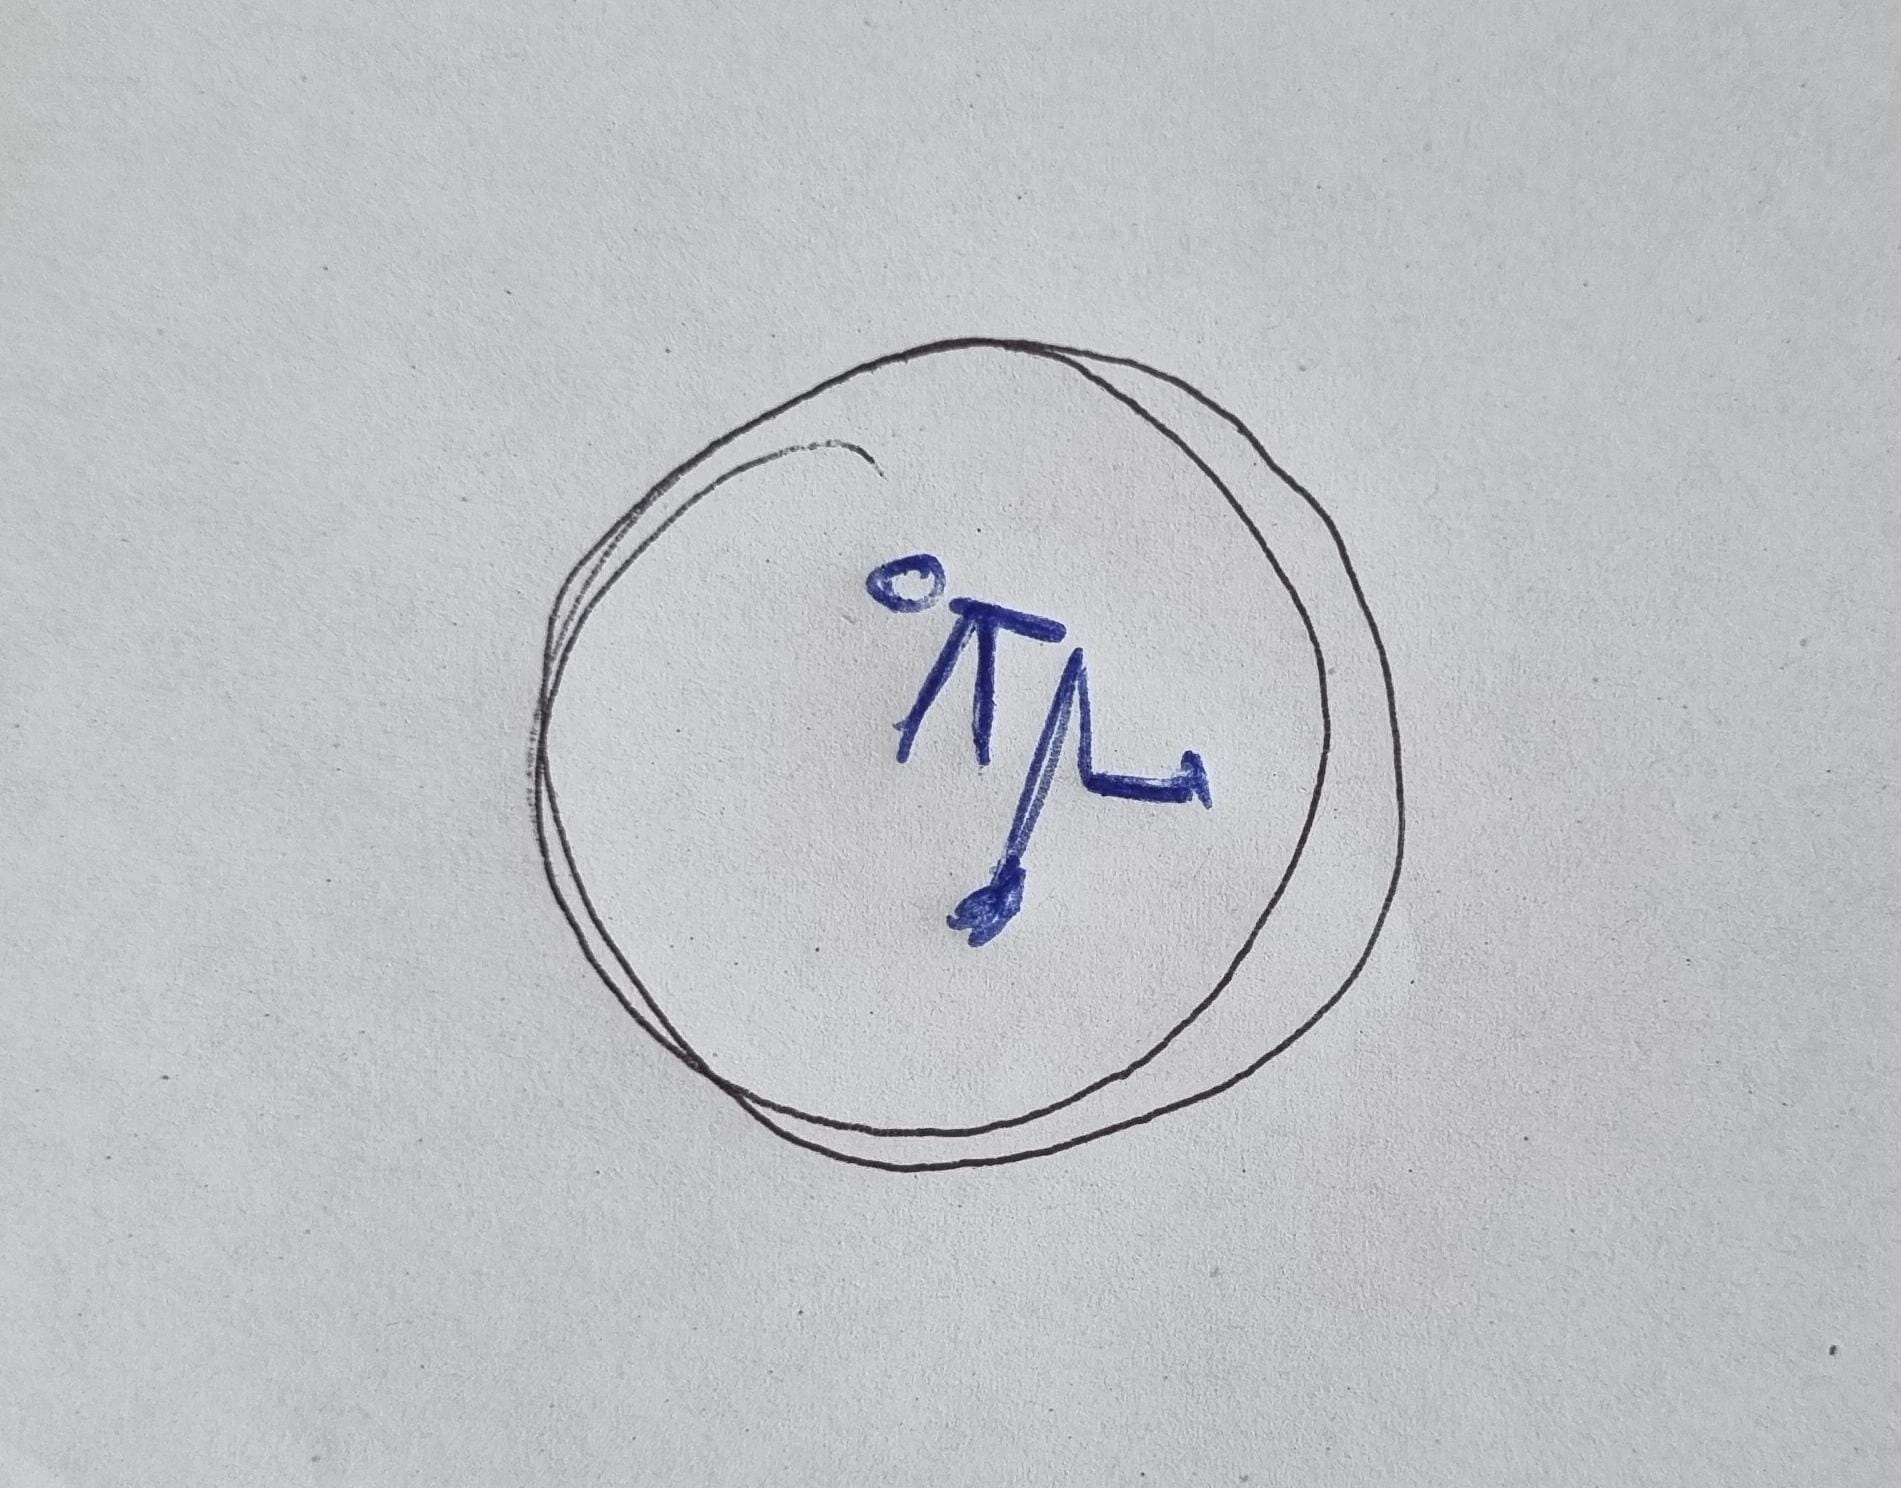
\includegraphics[width=0.6\textwidth,height=0.25\textheight,keepaspectratio]{images/Sprint3_4.jpg}
    \caption{Bewegungsresponsive Systeme: Performative Visual-Modulation}
    \label{fig:movement_responsive}
\end{figure}

% PLACEMENT: Sprint3.tex - Composite effect concepts
\begin{figure}[!htbp]
    \centering
    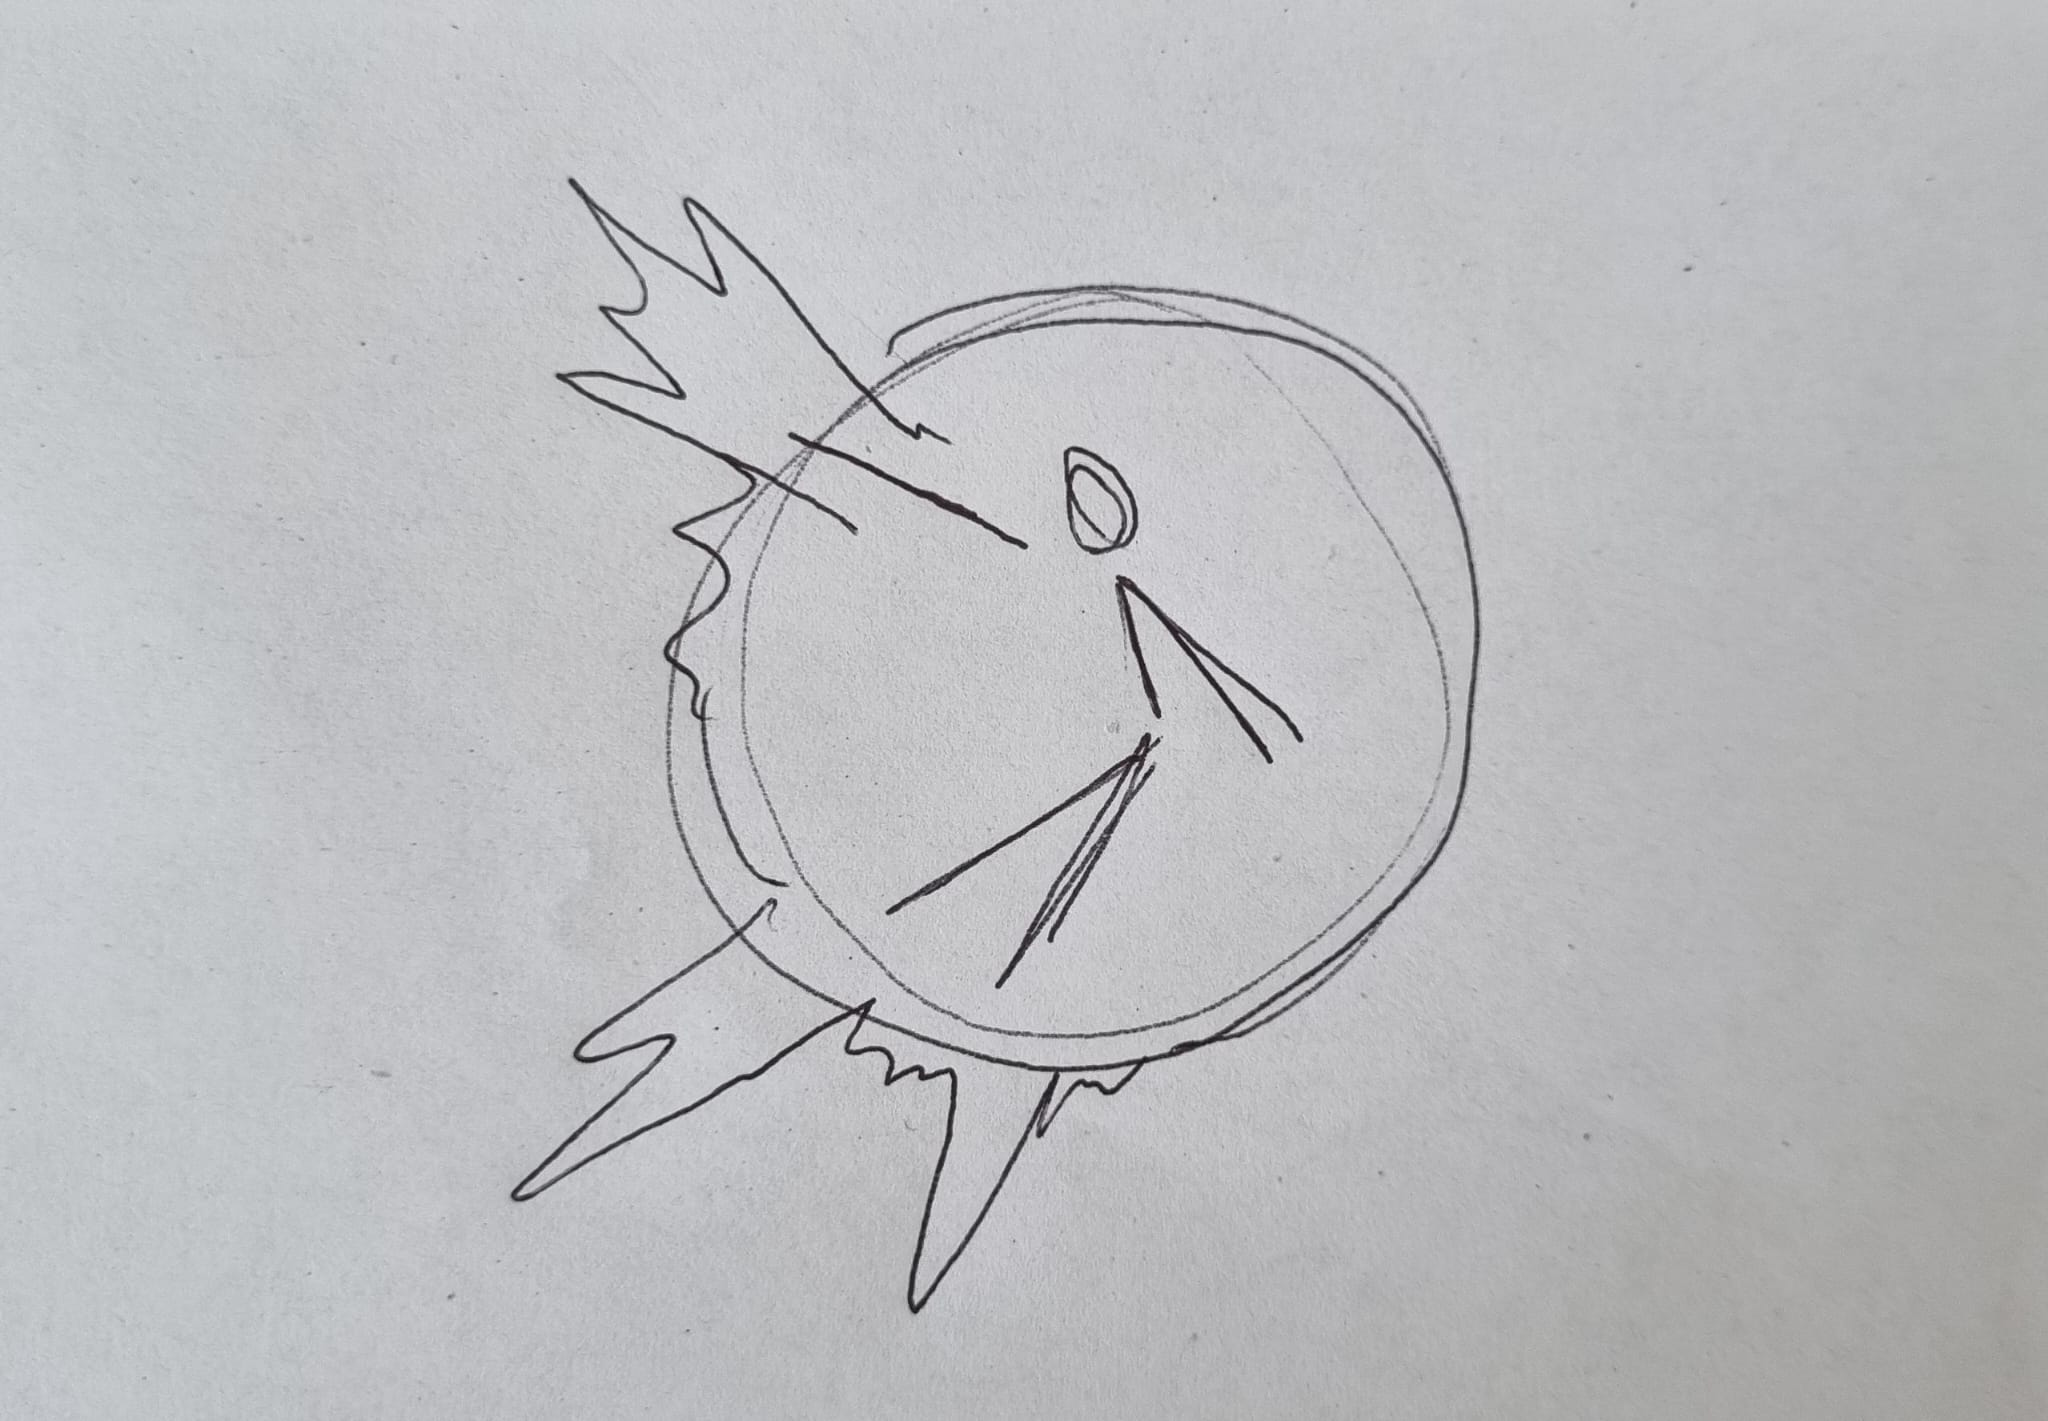
\includegraphics[width=0.6\textwidth,height=0.25\textheight,keepaspectratio]{images/Sprint3_5.jpg}
    \caption{Komposit-Effekte: Multi-Layer-Visual-Orchestrierung}
    \label{fig:composite_effects}
\end{figure}

% Sprint 4 figures
\begin{figure}[!htbp]
    \centering
    % \includegraphics[width=0.6\textwidth,height=0.25\textheight,keepaspectratio]{images/debug_visualization.png}
    \caption{Debug-Visualisierung: MediaPipe Skeleton-Nodes mit Confidence-Overlays}
    \label{fig:debug_viz}
\end{figure}

% Sprint 5 figures
% PLACEMENT: Systemarchitektur_und_Ergebnisse.tex or Sprint5.tex - Main system interface
\begin{figure}[!htbp]
    \centering
    \includegraphics[width=0.6\textwidth,height=0.25\textheight,keepaspectratio]{images/docupictures/Finished_MediaPipeContainer_mitErklärungen.png}
    \caption{M.A.S.K. MediaPipe-Container Haupt-Interface: Integration mit Debug-Visualisierung und Erklärungen}
    \label{fig:main_interface}
\end{figure}

% DUPLICATE IMAGE - COMMENTED OUT
% \begin{figure}[!htbp]
%     \centering
%     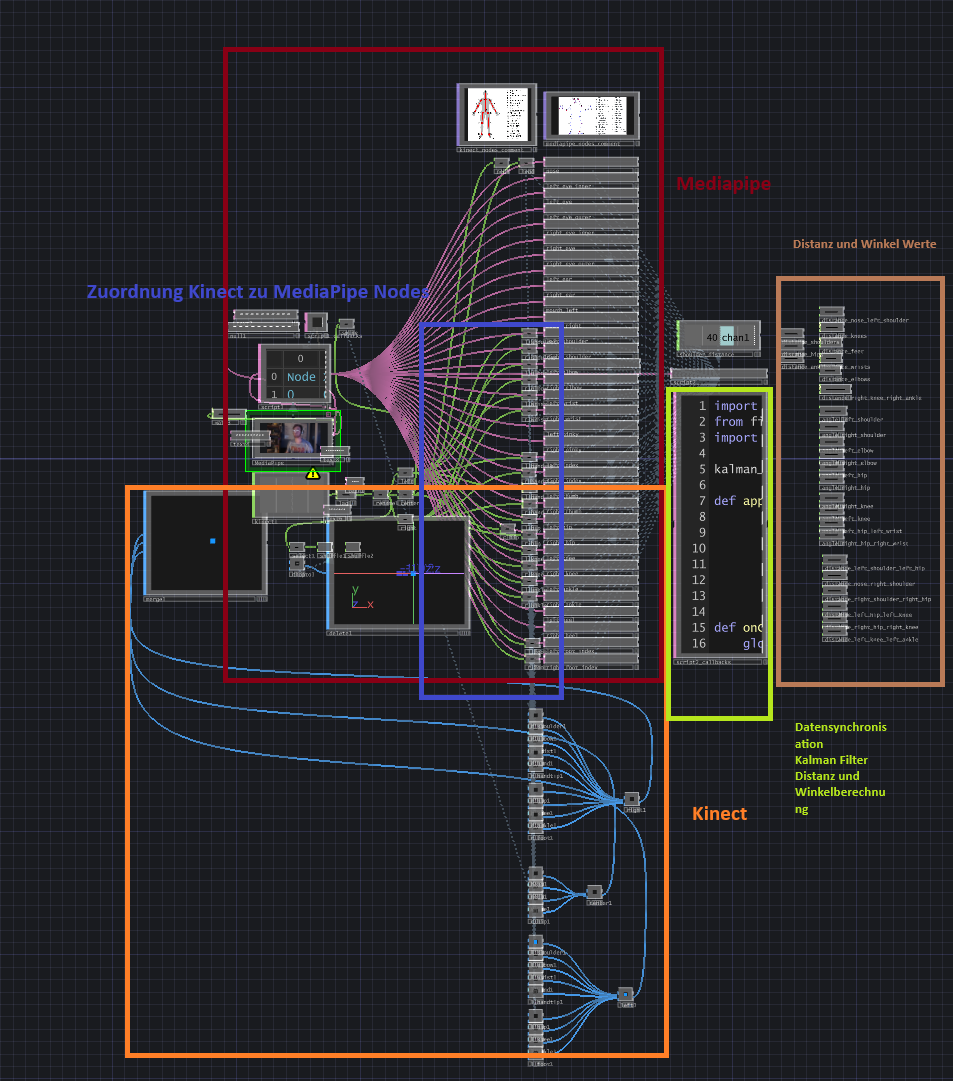
\includegraphics[width=0.6\textwidth,height=0.25\textheight,keepaspectratio]{images/docupictures/KinectMediaPipe_Testing.png}
%     \caption{Komparative Tracking-Tests: MediaPipe vs. Kinect Evaluation}
%     \label{fig:tracking_comparison}
% \end{figure}

% PLACEMENT: Systemarchitektur_und_Ergebnisse.tex - Technical implementation details
\begin{figure}[!htbp]
    \centering
    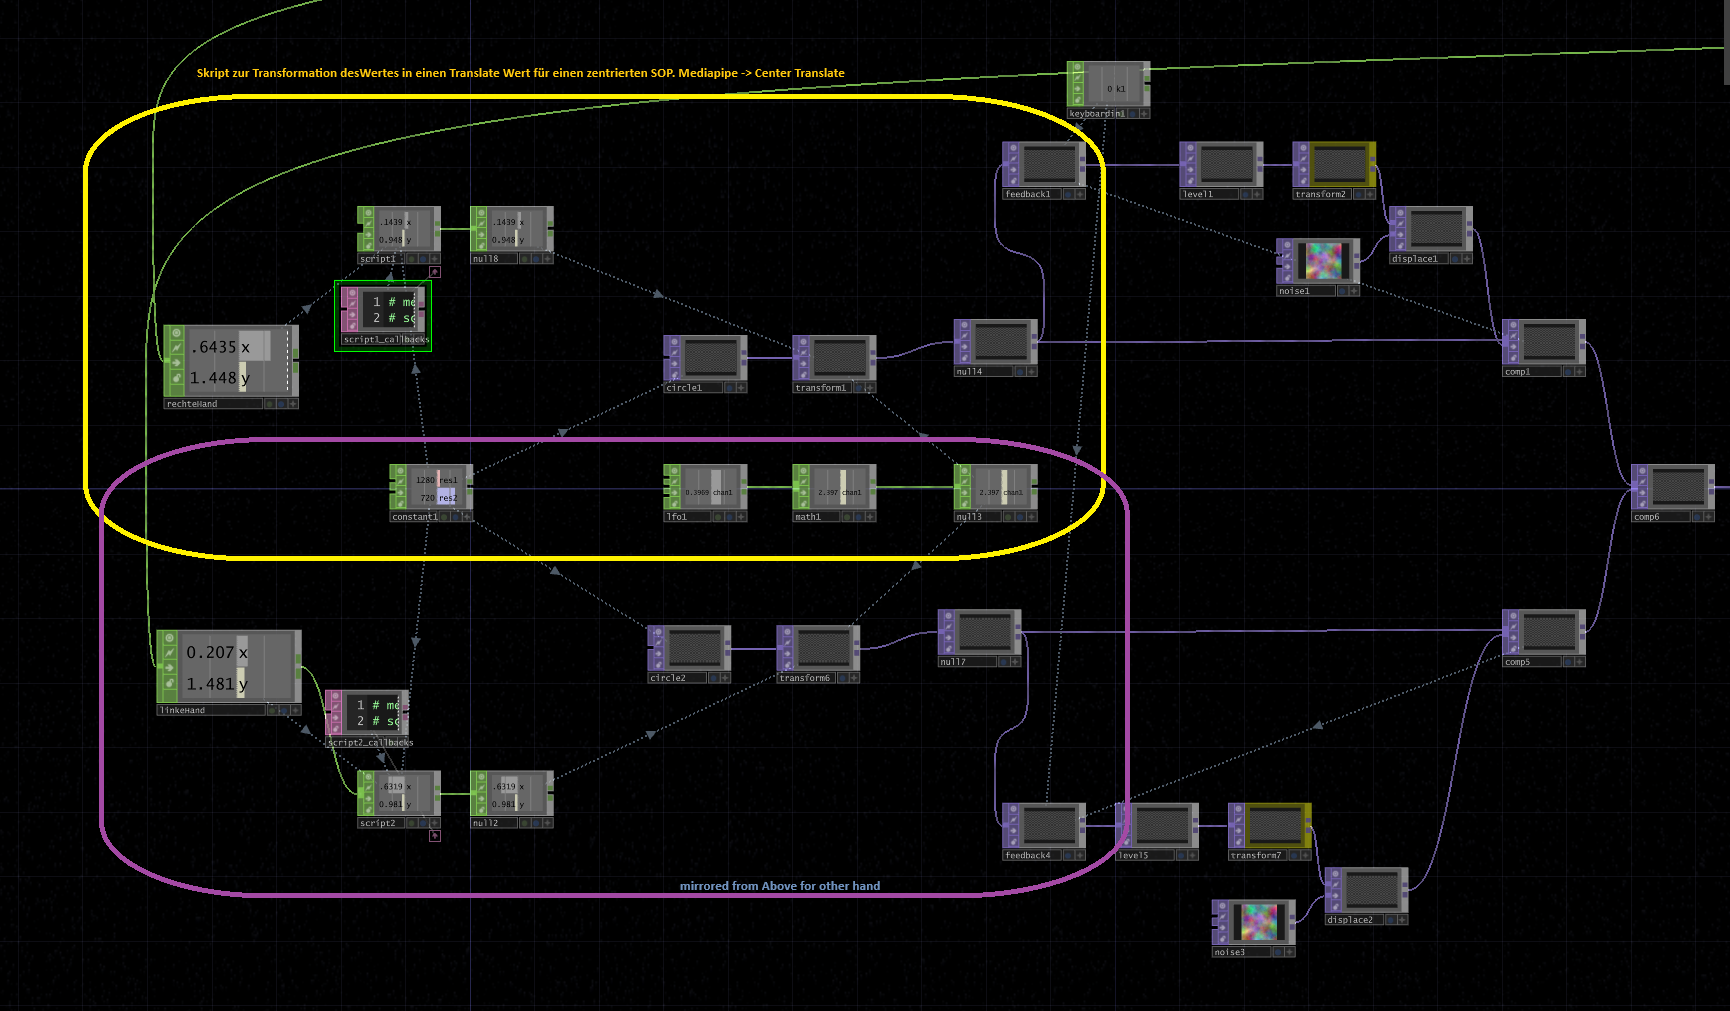
\includegraphics[width=0.6\textwidth,height=0.25\textheight,keepaspectratio]{images/docupictures/NodeXYzuSOPZentriertemTranslate.png}
    \caption{Koordinatentransformation: Node-XY zu zentralisiertem SOP-Translate}
    \label{fig:coordinate_transformation}
\end{figure}

% PLACEMENT: Sprint4.tex or Demonstration.tex - Visual effect implementation
\begin{figure}[!htbp]
    \centering
    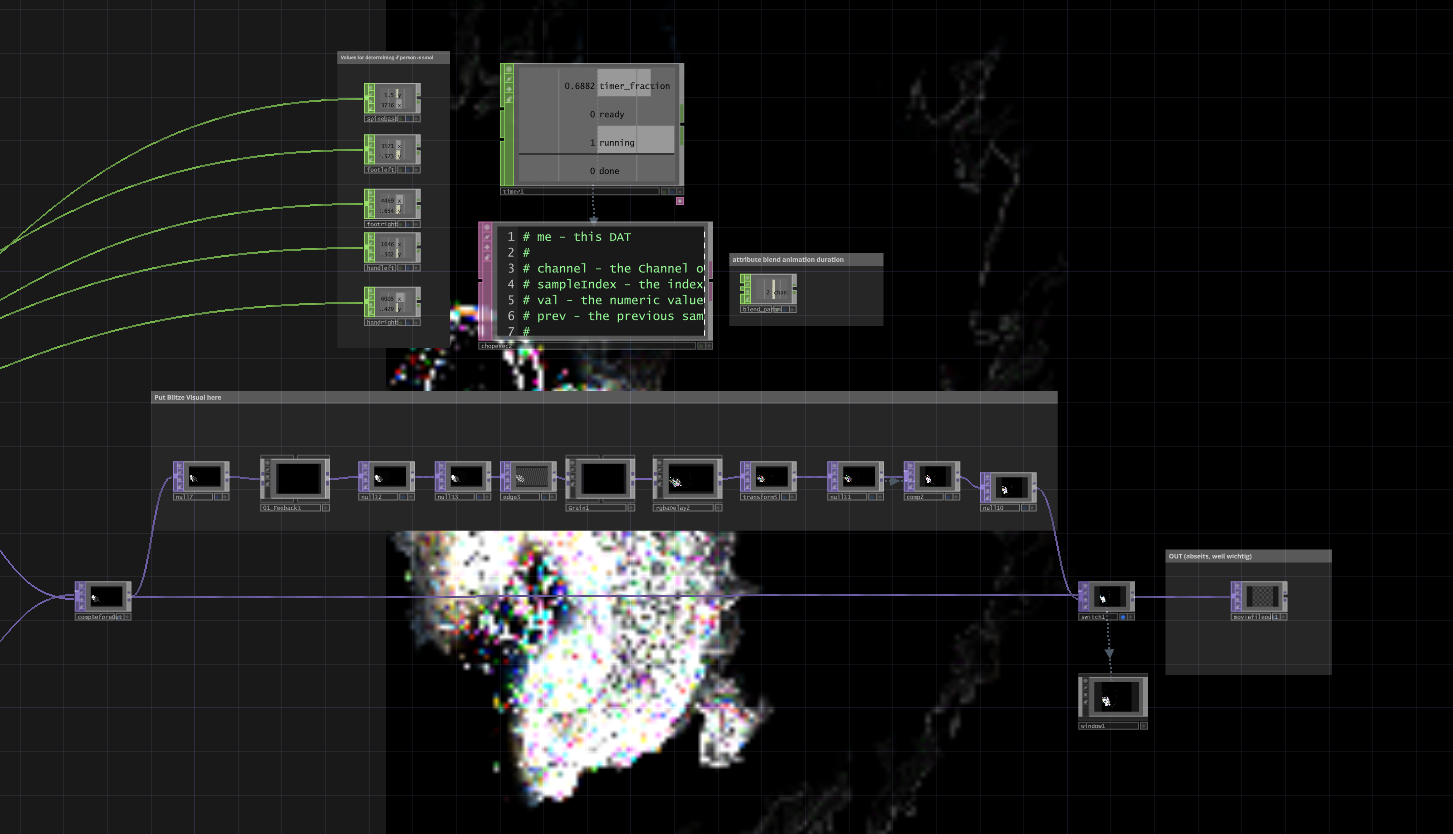
\includegraphics[width=0.6\textwidth,height=0.25\textheight,keepaspectratio]{images/docupictures/NoisyBlob_animatedSwitchzwischenBlitzUndNichtBlitzBeiTrackingTrigger.png}
    \caption{NoisyBlob Adaptive Visual-Switch: Animierte Zustandsmaschine mit Tracking-Triggern}
    \label{fig:animated_switch}
\end{figure}

% PLACEMENT: Sprint5.tex or Systemarchitektur_und_Ergebnisse.tex - Core pipeline implementation
\begin{figure}[!htbp]
    \centering
    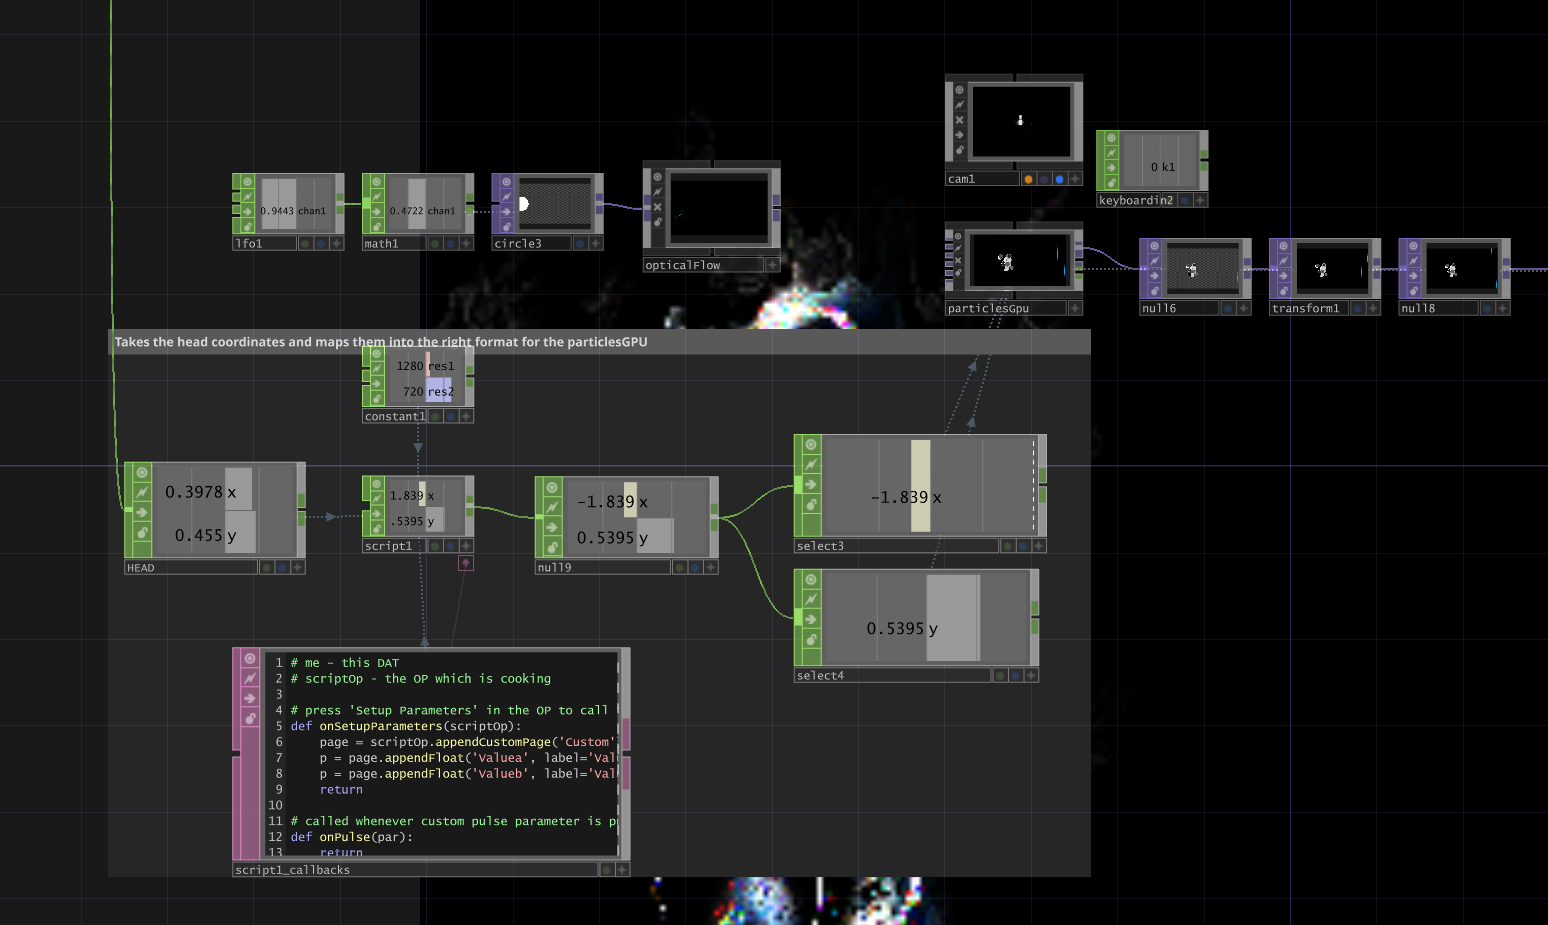
\includegraphics[width=0.6\textwidth,height=0.25\textheight,keepaspectratio]{images/docupictures/NoisyBlob_HEAD_to_ParticleGPU_Translate.png}
    \caption{NoisyBlob ParticleGPU-Pipeline: Head-Node zu ParticleGPU Translation}
    \label{fig:particle_translation}
\end{figure}

% PLACEMENT: Sprint6.tex or Systemarchitektur_und_Ergebnisse.tex - 64-spike system mathematics
\begin{figure}[!htbp]
    \centering
    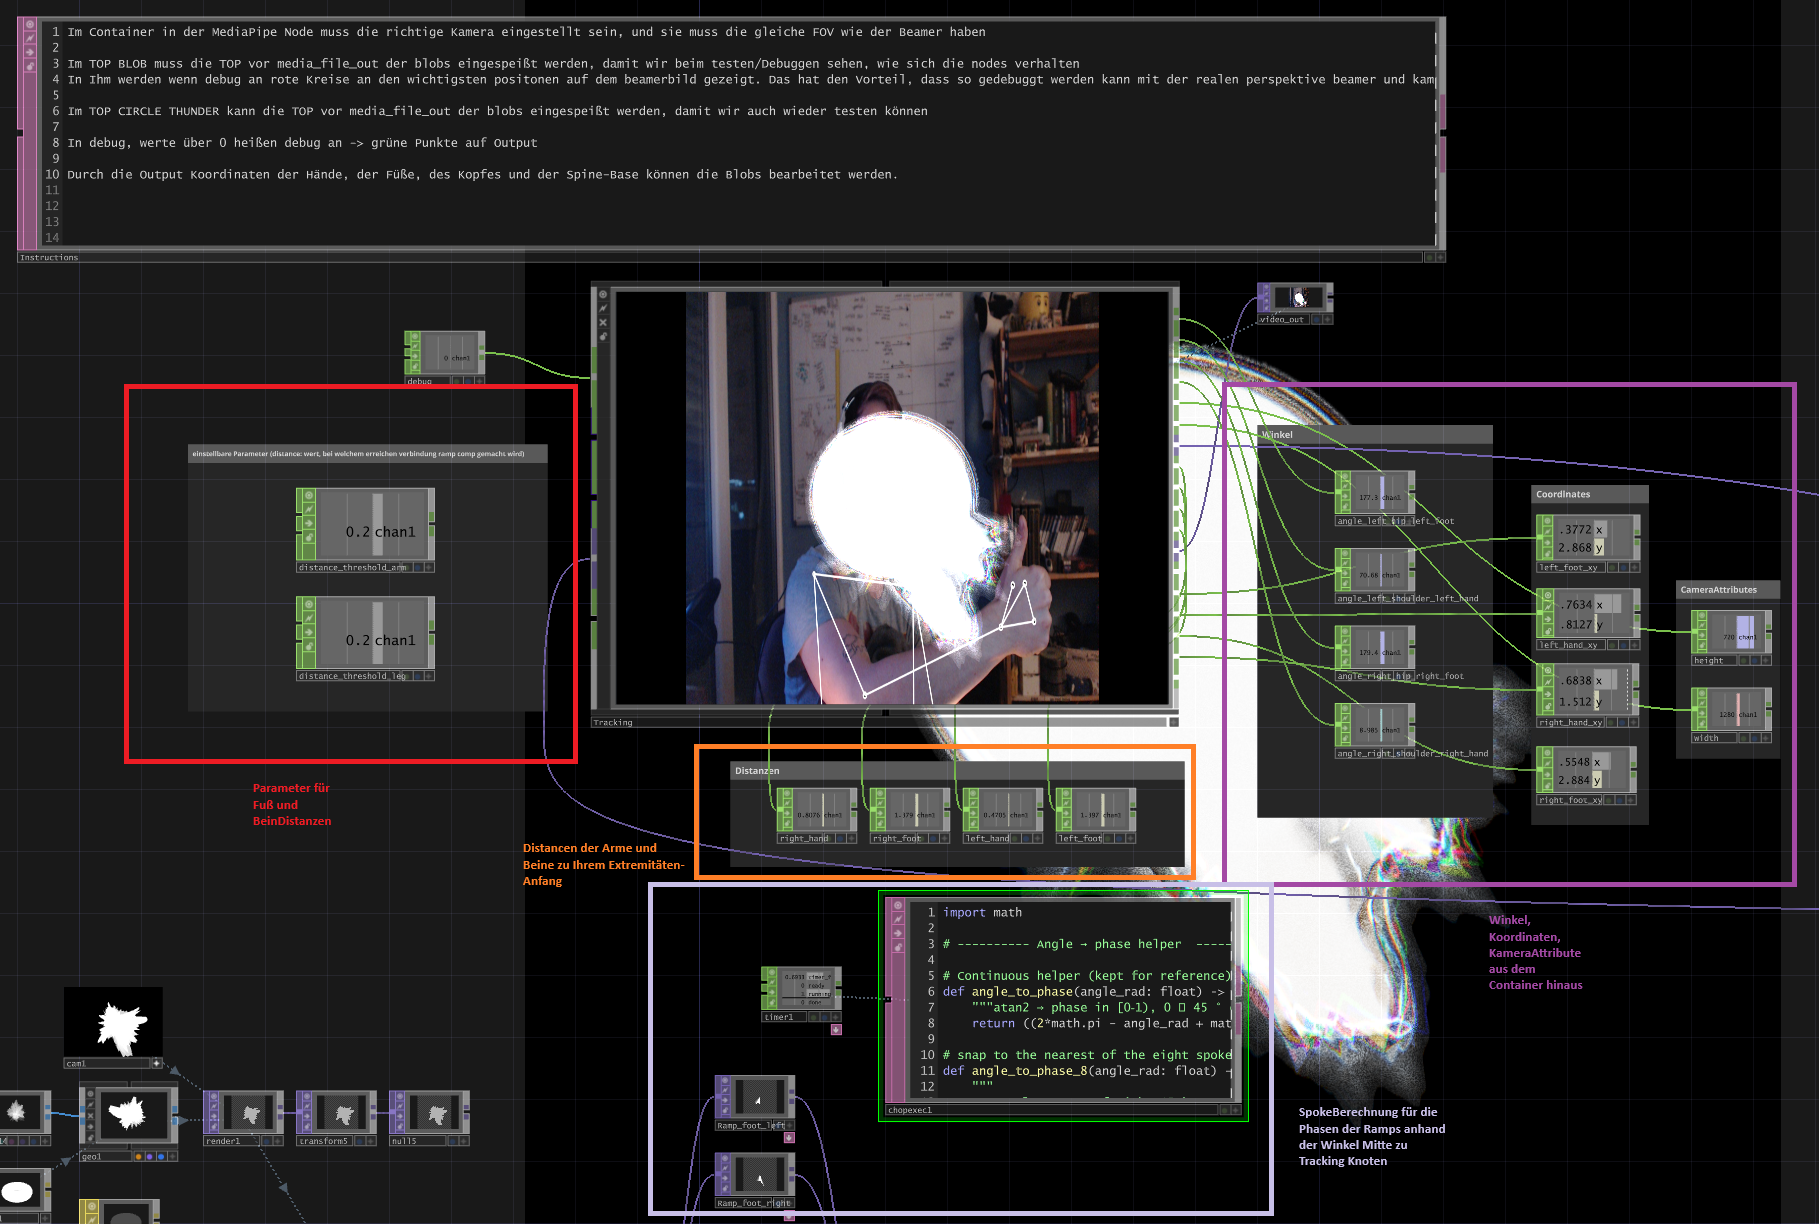
\includegraphics[width=0.6\textwidth,height=0.25\textheight,keepaspectratio]{images/docupictures/TopDown_KreisZuRampsParametisierteBerechnungen.png}
    \caption{64-Spike Radialsystem: Polar-Koordinaten-Berechnung mit parametrisierter Ramp-Generation}
    \label{fig:radial_spike_system}
\end{figure}

% Systemarchitektur und Ergebnisse figures
% DUPLICATE IMAGE - COMMENTED OUT
% \begin{figure}[!htbp]
%     \centering
%     \includegraphics[width=0.6\textwidth,height=0.25\textheight,keepaspectratio]{images/docupictures/Finished_MediaPipeContainer_mitErklärungen.png}
%     \caption{MediaPipe-Container: Vollst�ndige Pipeline-Architektur mit Erkl�rungen}
%     \label{fig:mediapipe_architecture}
% \end{figure}

% DUPLICATE IMAGE - COMMENTED OUT
% \begin{figure}[!htbp]
%     \centering
%     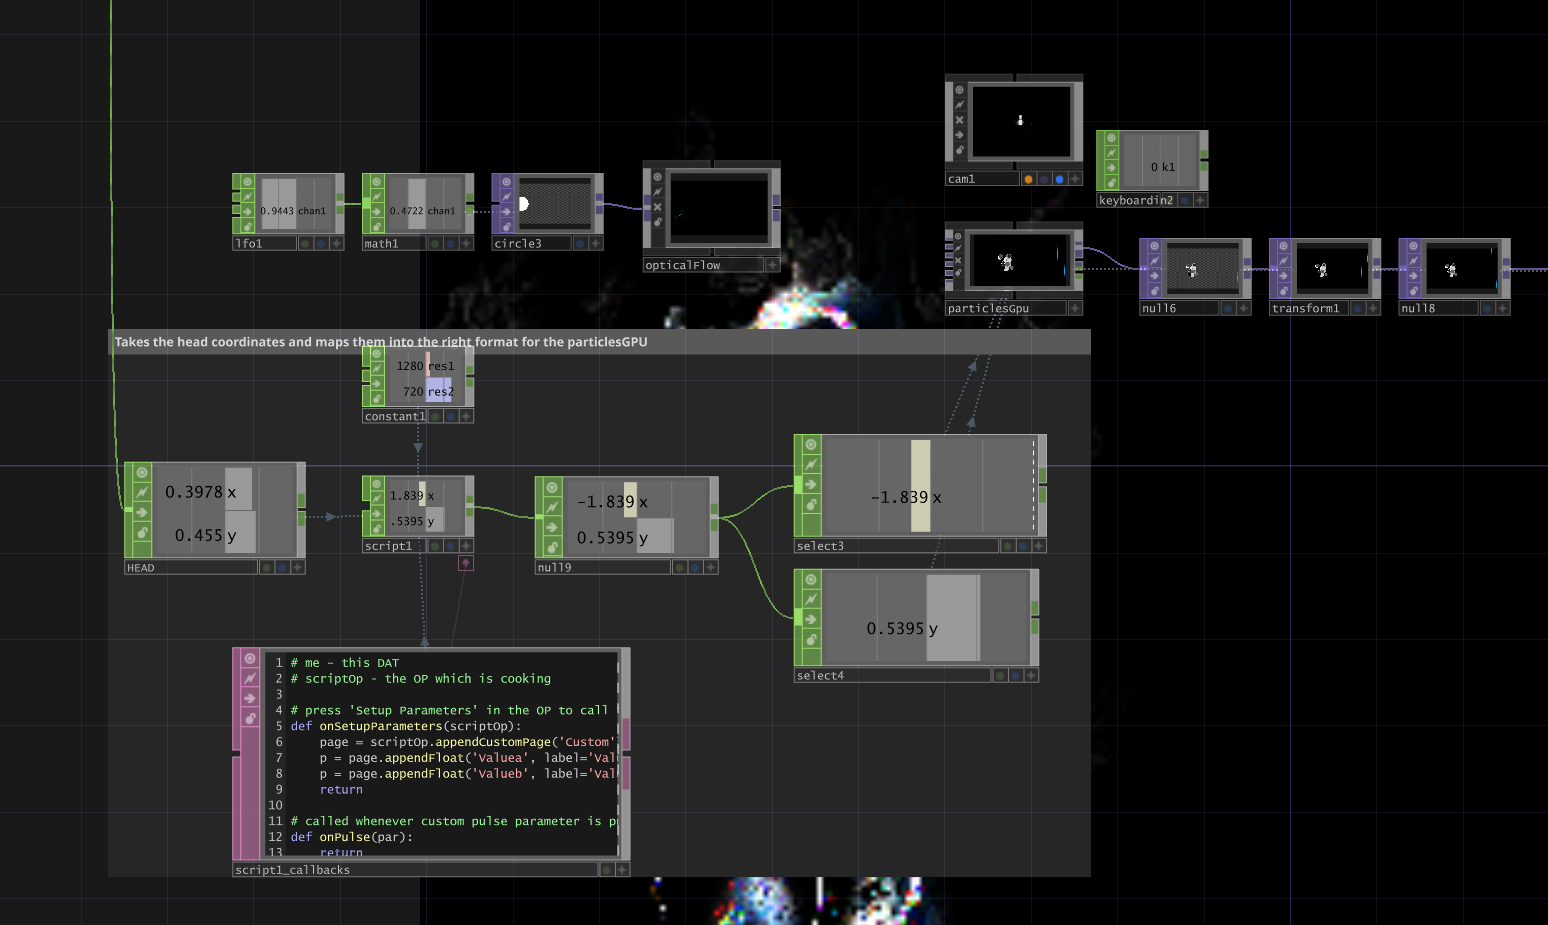
\includegraphics[width=0.6\textwidth,height=0.25\textheight,keepaspectratio]{images/docupictures/NoisyBlob_HEAD_to_ParticleGPU_Translate.png}
%     \caption{Hand-Feuer-Implementation: ParticleGPU-basierte Echtzeit-Responsivit�t}
%     \label{fig:hand_fire_system}
% \end{figure}

% DUPLICATE IMAGE - COMMENTED OUT
% \begin{figure}[!htbp]
%     \centering
%     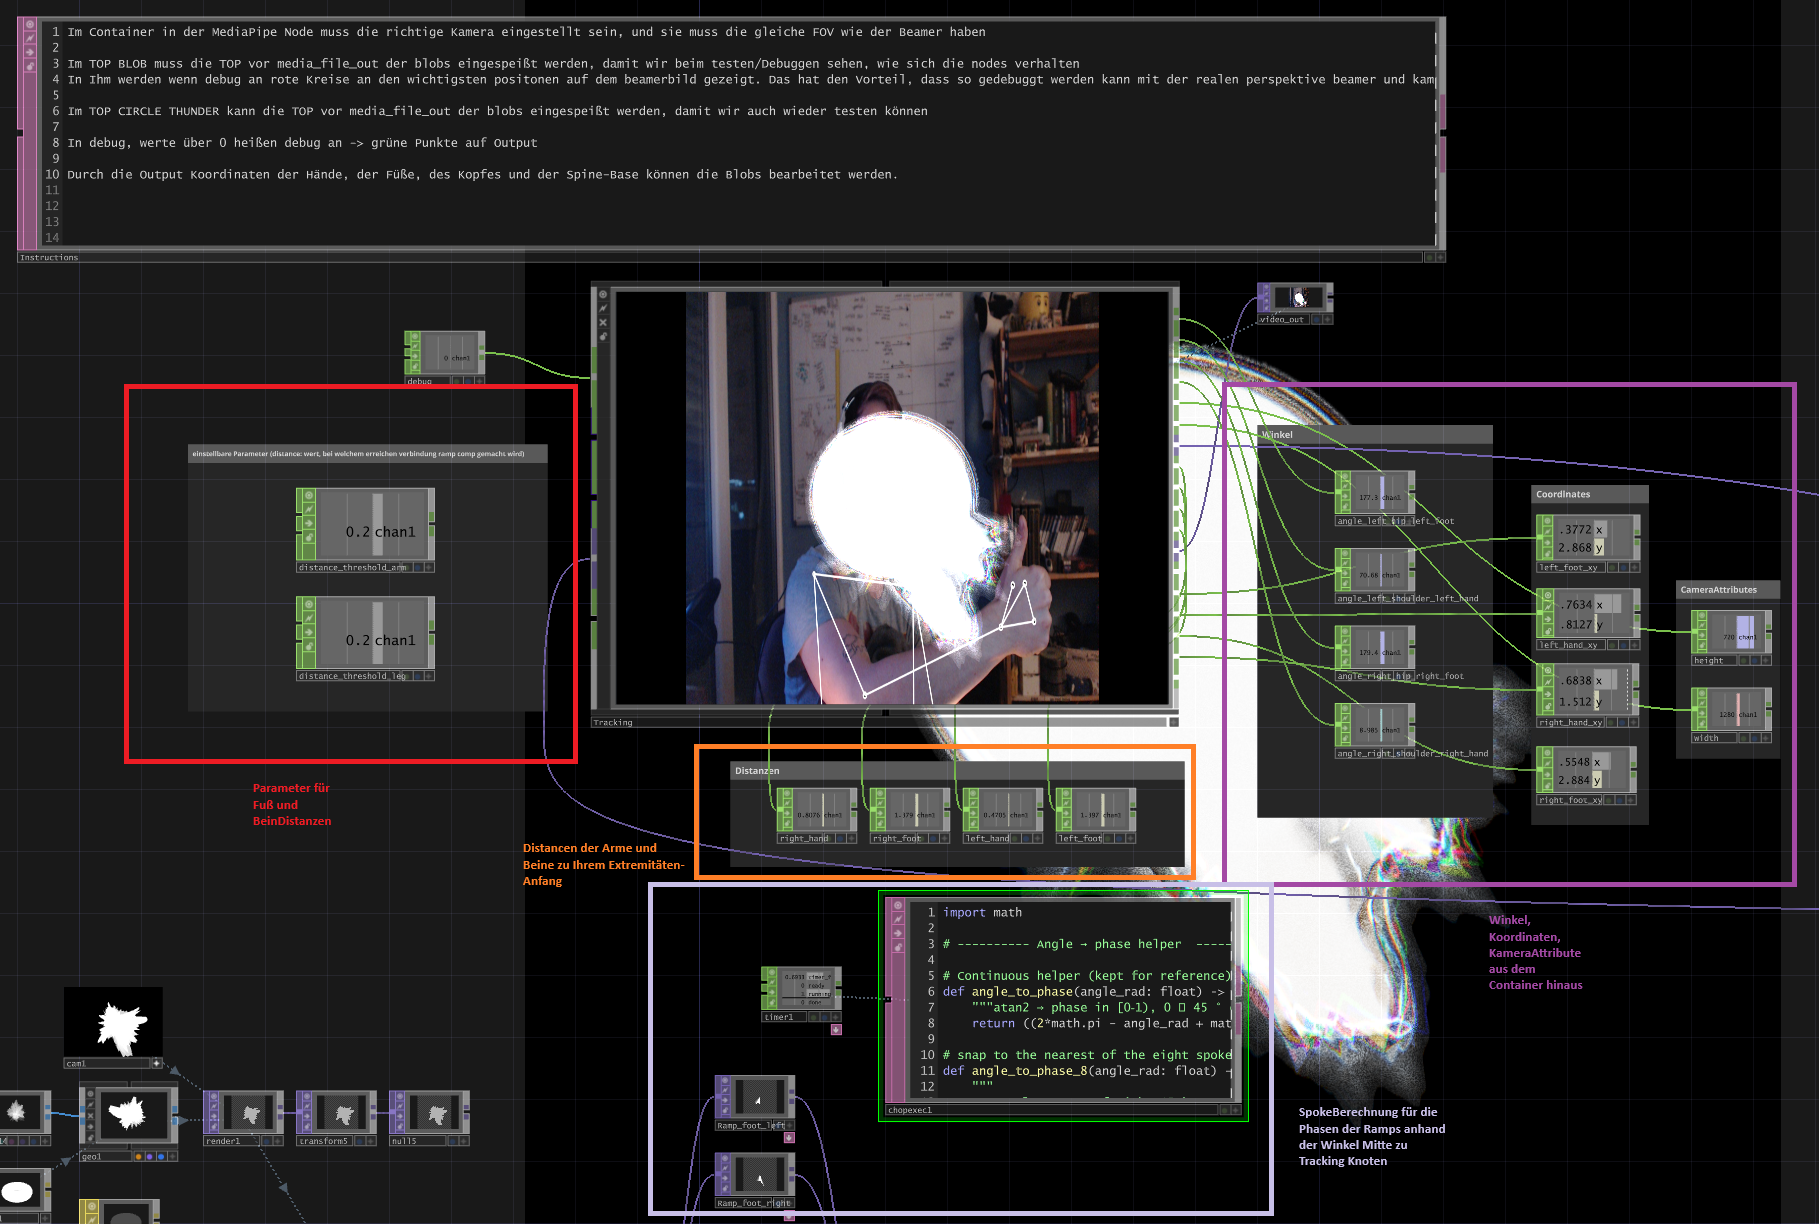
\includegraphics[width=0.6\textwidth,height=0.25\textheight,keepaspectratio]{images/docupictures/TopDown_KreisZuRampsParametisierteBerechnungen.png}
%     \caption{64-Spike-System: Polar-Koordinaten-Mapping mit 5,625� Aufl�sung}
%     \label{fig:spike_system_production}
% \end{figure}

% Entwicklungsprozess figures
% DUPLICATE IMAGE - COMMENTED OUT
% \begin{figure}[!htbp]
%     \centering
%     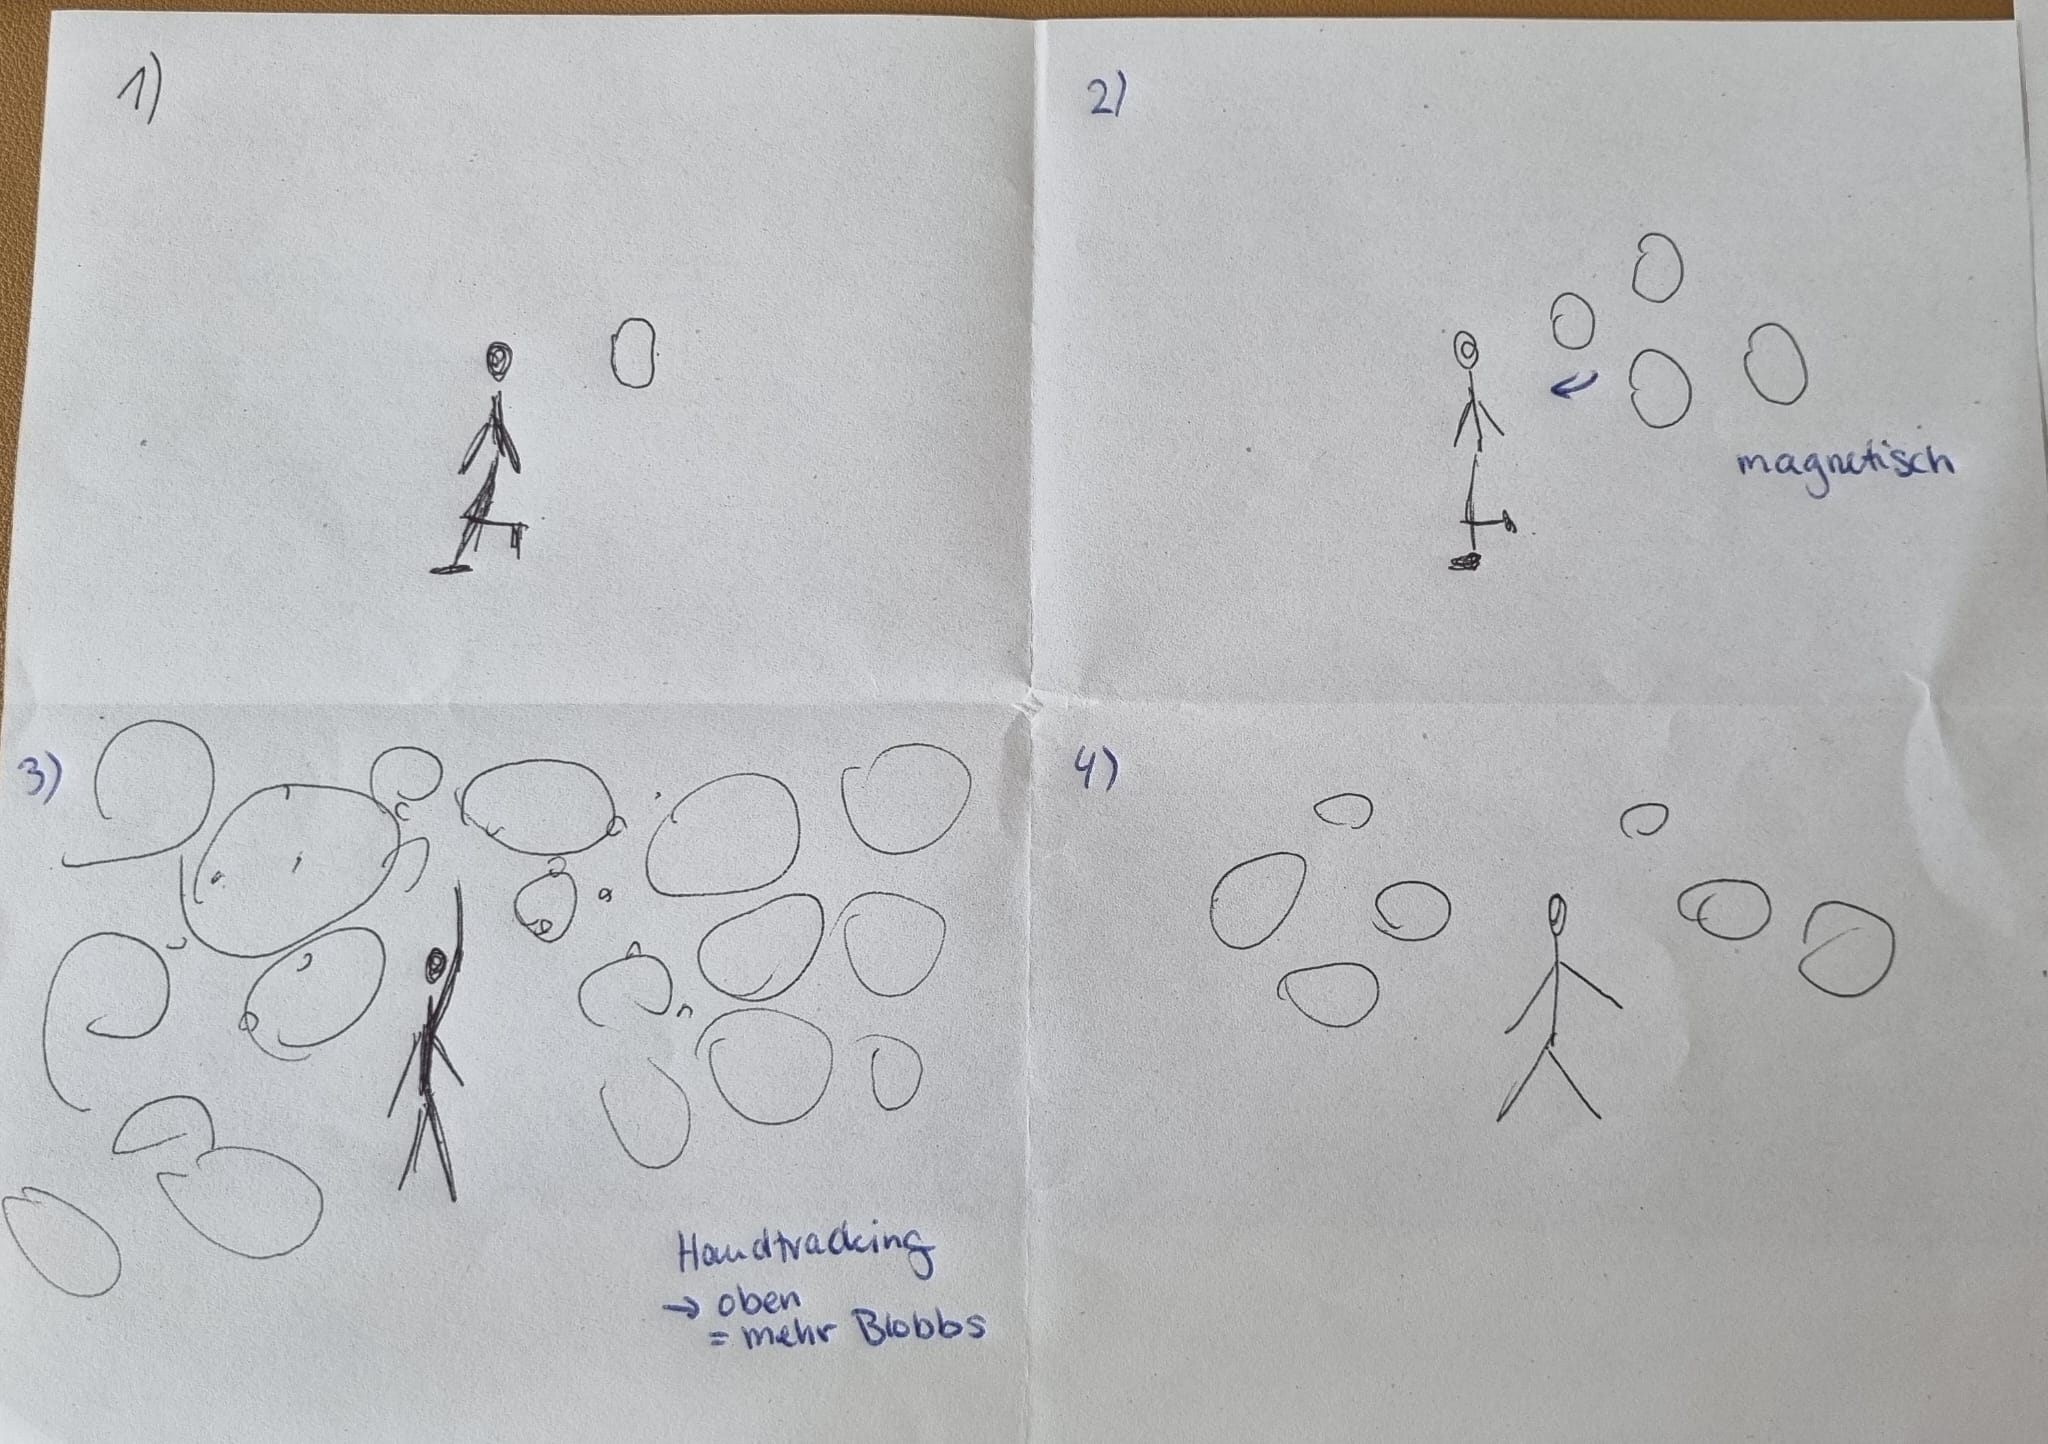
\includegraphics[width=0.6\textwidth,height=0.25\textheight,keepaspectratio]{images/Sprint3_1.jpg}
%     \caption{Designkonzept: Skalierungsresponsive Visual-Transformation}
%     \label{fig:design_evolution}
% \end{figure}

% PLACEHOLDER IMAGE - COMMENTED OUT (DUPLICATE MASK.png usage)
% TODO: Create actual infrared pipeline diagram
% \begin{figure}[!htbp]
%     \centering
%     % TODO: Replace with actual infrared pipeline diagram
%     % \includegraphics[width=0.6\textwidth,height=0.25\textheight,keepaspectratio]{images/infrared_pipeline_diagram.png}
%     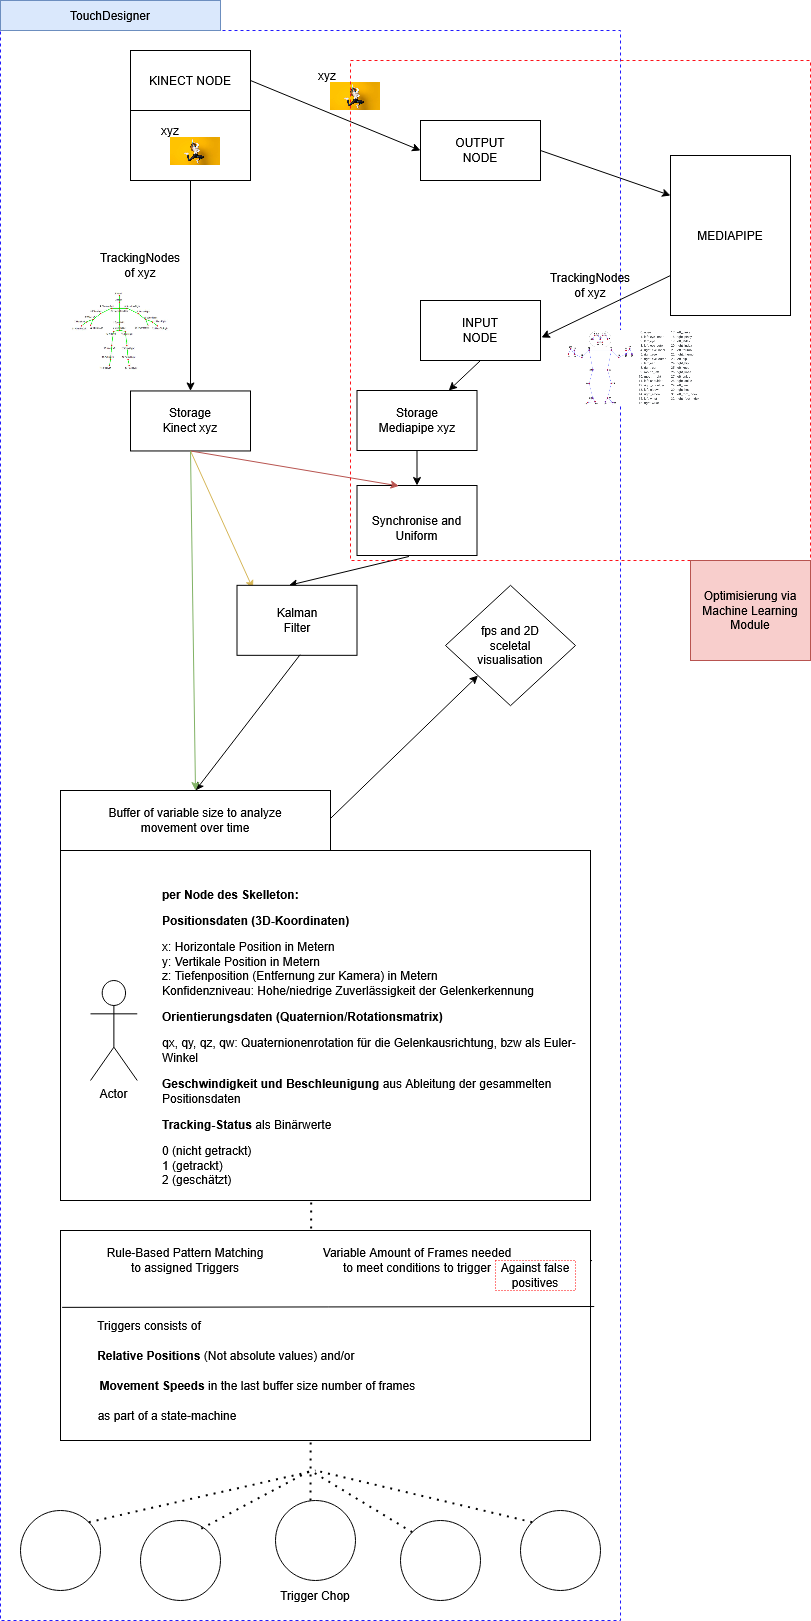
\includegraphics[width=0.6\textwidth,height=0.25\textheight,keepaspectratio]{images/MASK.png}
%     \caption{Infrarot-MediaPipe-Pipeline: Technische L�sung f�r Produktionsumgebungen (Platzhalter - spezifisches Infrarot-Pipeline-Diagramm erforderlich)}
%     \label{fig:infrared_solution}
% \end{figure}

% Demonstration figures
% DUPLICATE IMAGE - COMMENTED OUT
% \begin{figure}[!htbp]
%     \centering
%     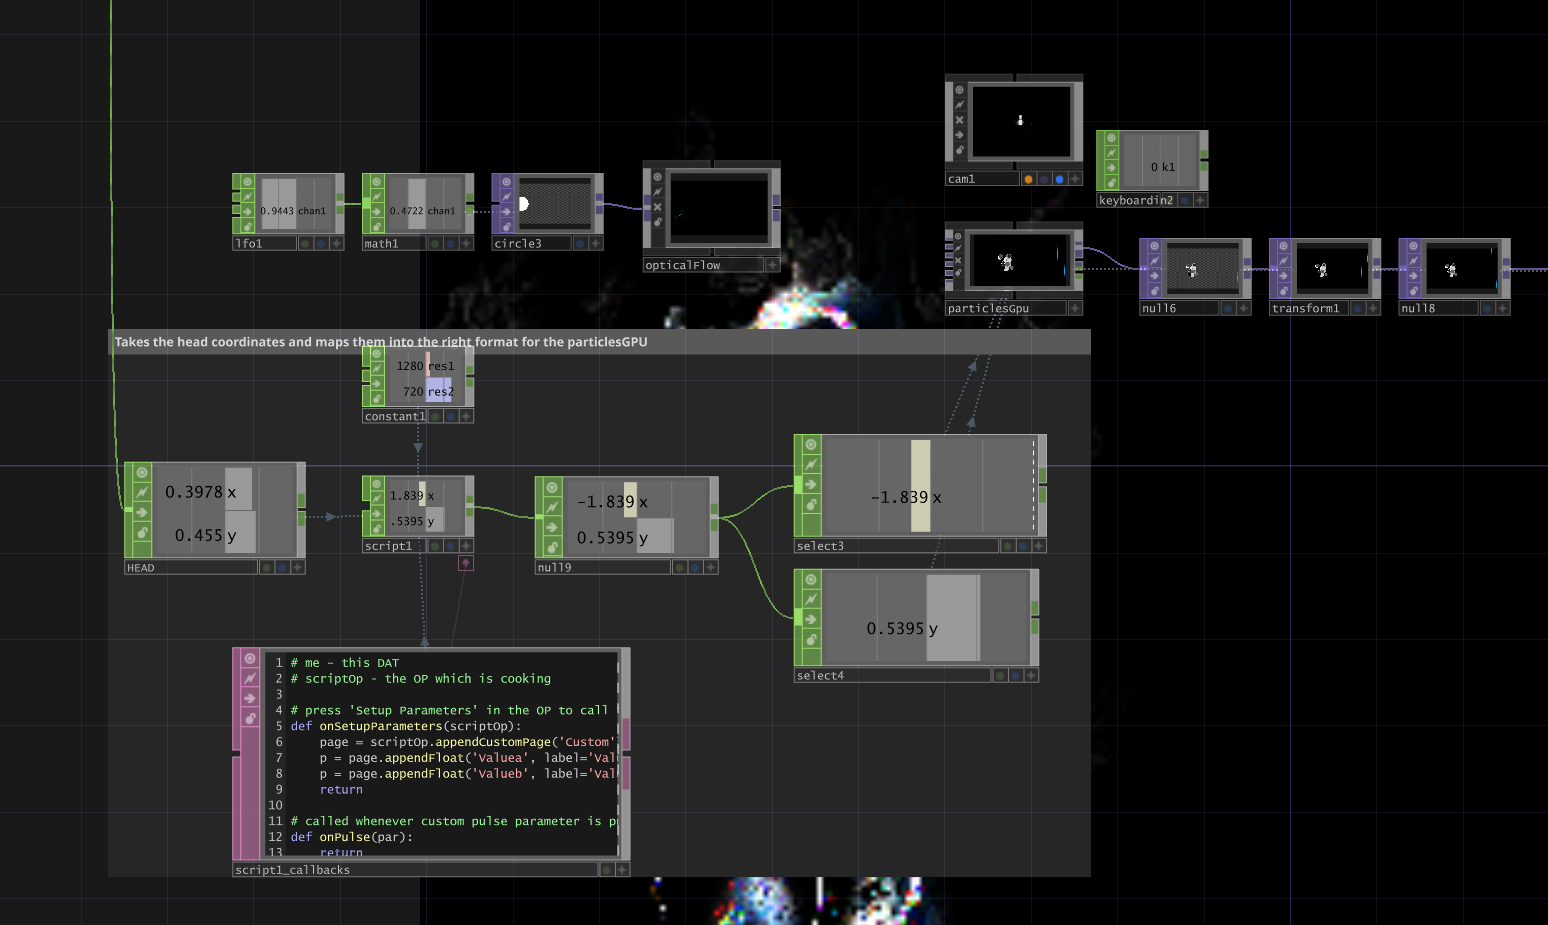
\includegraphics[width=0.6\textwidth,height=0.25\textheight,keepaspectratio]{images/docupictures/NoisyBlob_HEAD_to_ParticleGPU_Translate.png}
%     \caption{NoisyBlob Hand-Feuer-Effekte: Blaue Partikel folgen Handbewegungen in Echtzeit}
%     \label{fig:particle_hands}
% \end{figure}

% DUPLICATE IMAGE - COMMENTED OUT
% \begin{figure}[!htbp]
%     \centering
%     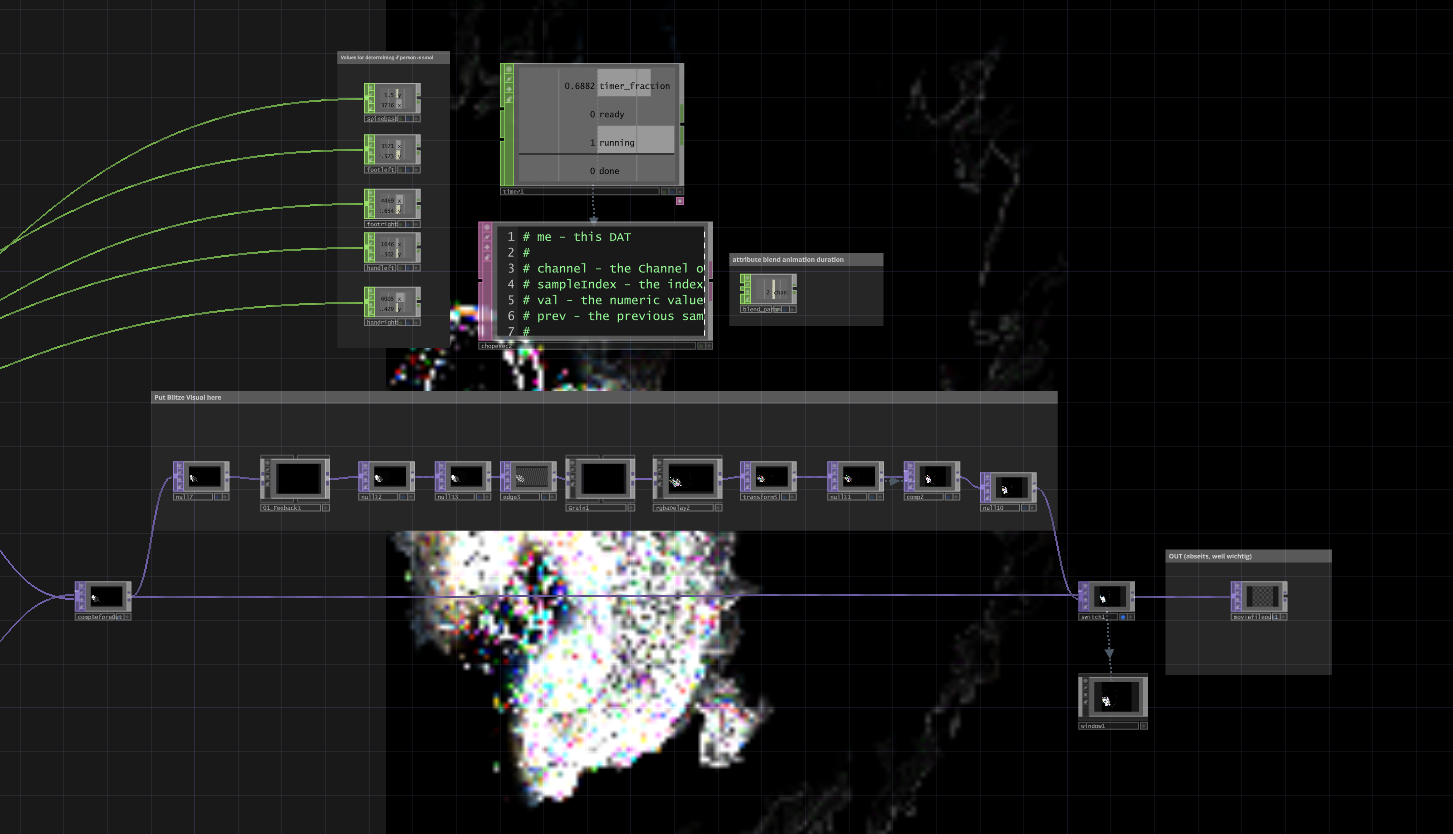
\includegraphics[width=0.6\textwidth,height=0.25\textheight,keepaspectratio]{images/docupictures/NoisyBlob_animatedSwitchzwischenBlitzUndNichtBlitzBeiTrackingTrigger.png}
%     \caption{NoisyBlob Adaptive Kopfpartikel: Zustandswechsel basierend auf Handposition relativ zur Schulter}
%     \label{fig:relative_switch}
% \end{figure}

% DUPLICATE IMAGE - COMMENTED OUT
% \begin{figure}[!htbp]
%     \centering
%     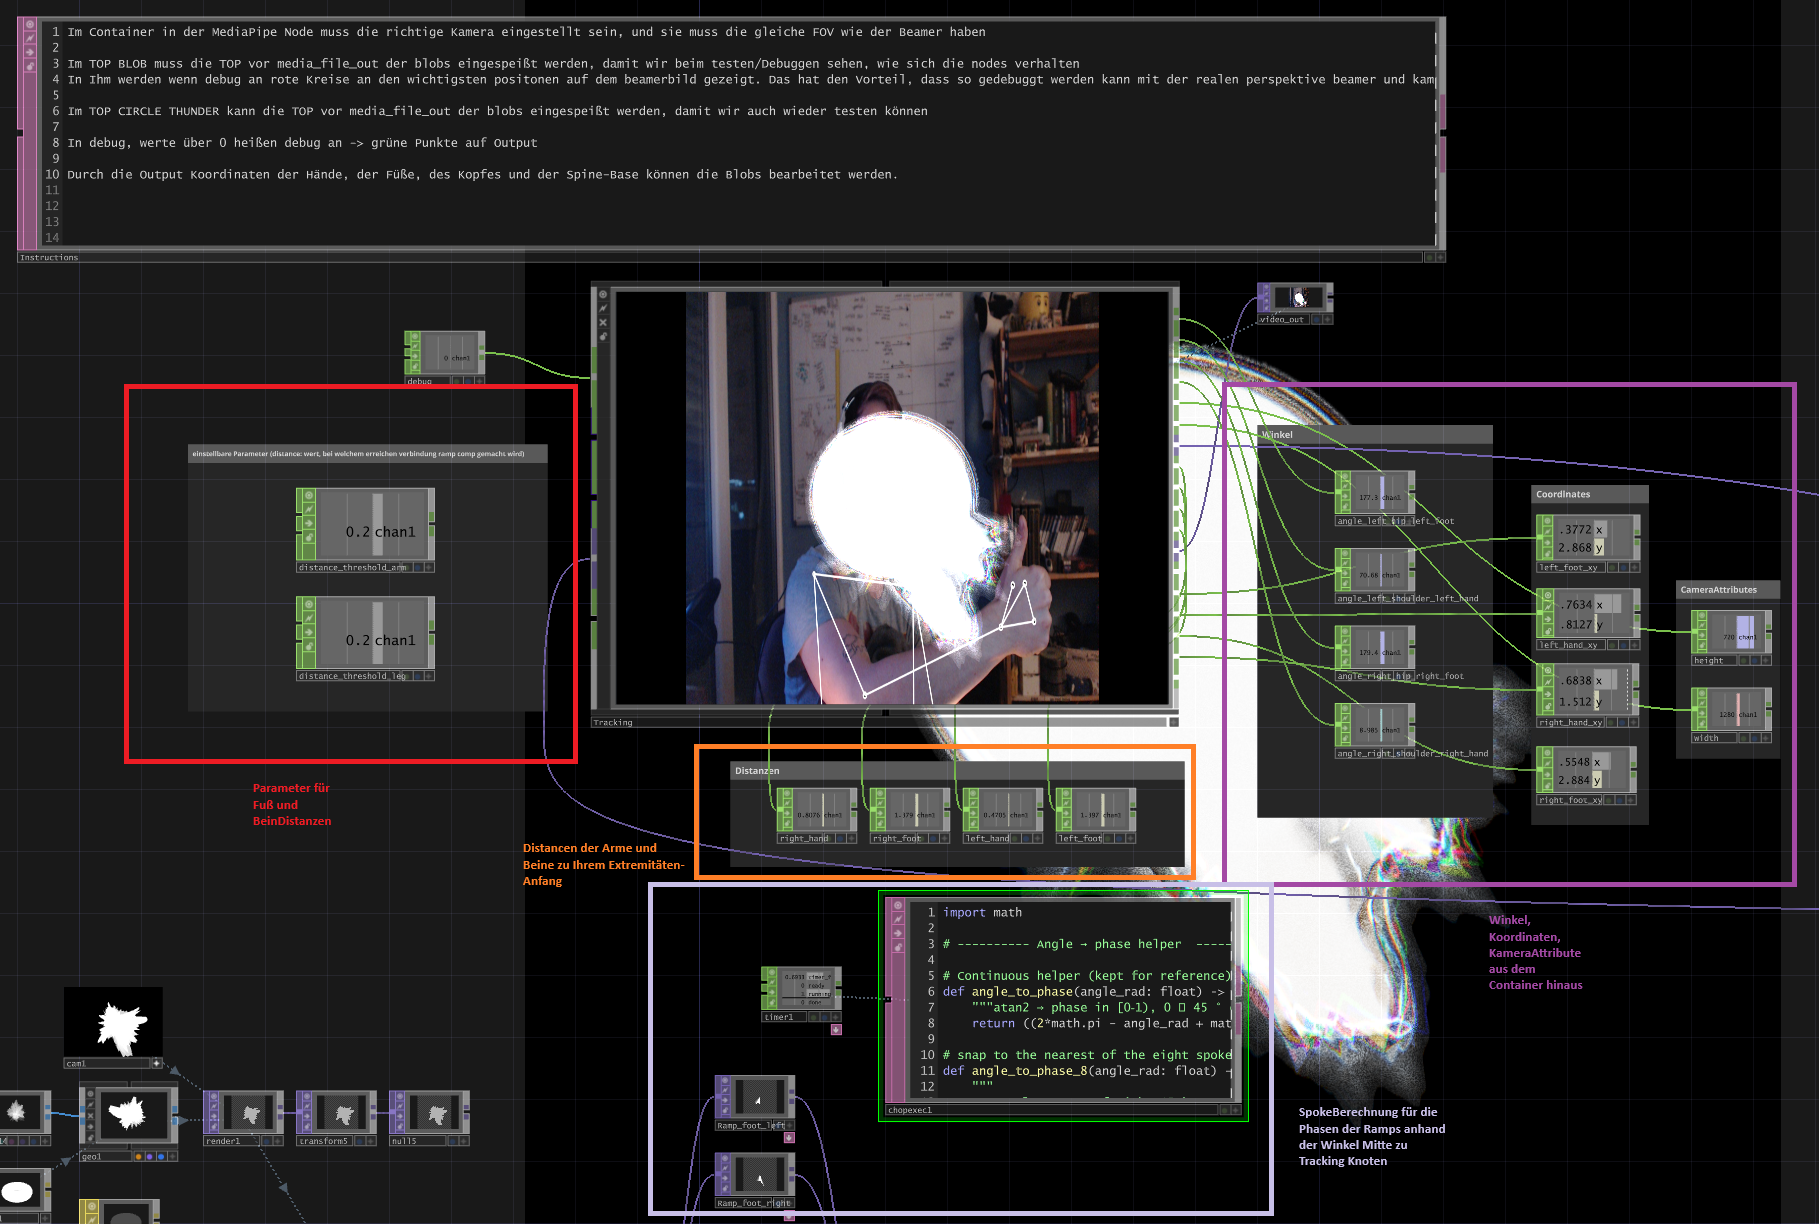
\includegraphics[width=0.6\textwidth,height=0.25\textheight,keepaspectratio]{images/docupictures/TopDown_KreisZuRampsParametisierteBerechnungen.png}
%     \caption{64-Spike Radialsystem: Winkelaufl�sung von 5,625� f�r pr�zise Extremit�tenerkennung}
%     \label{fig:spike_system}
% \end{figure}

% DUPLICATE IMAGE - COMMENTED OUT
% \begin{figure}[!htbp]
%     \centering
%     \includegraphics[width=0.6\textwidth,height=0.25\textheight,keepaspectratio]{images/docupictures/Finished_MediaPipeContainer_mitErklärungen.png}
%     \caption{MediaPipe-Container Debug-Visualisierung: Skelett-Erkennung im Infrarot-Modus mit Erklärungen}
%     \label{fig:debug_circles}
% \end{figure}

% DUPLICATE IMAGE - COMMENTED OUT
% \begin{figure}[!htbp]
%     \centering
%     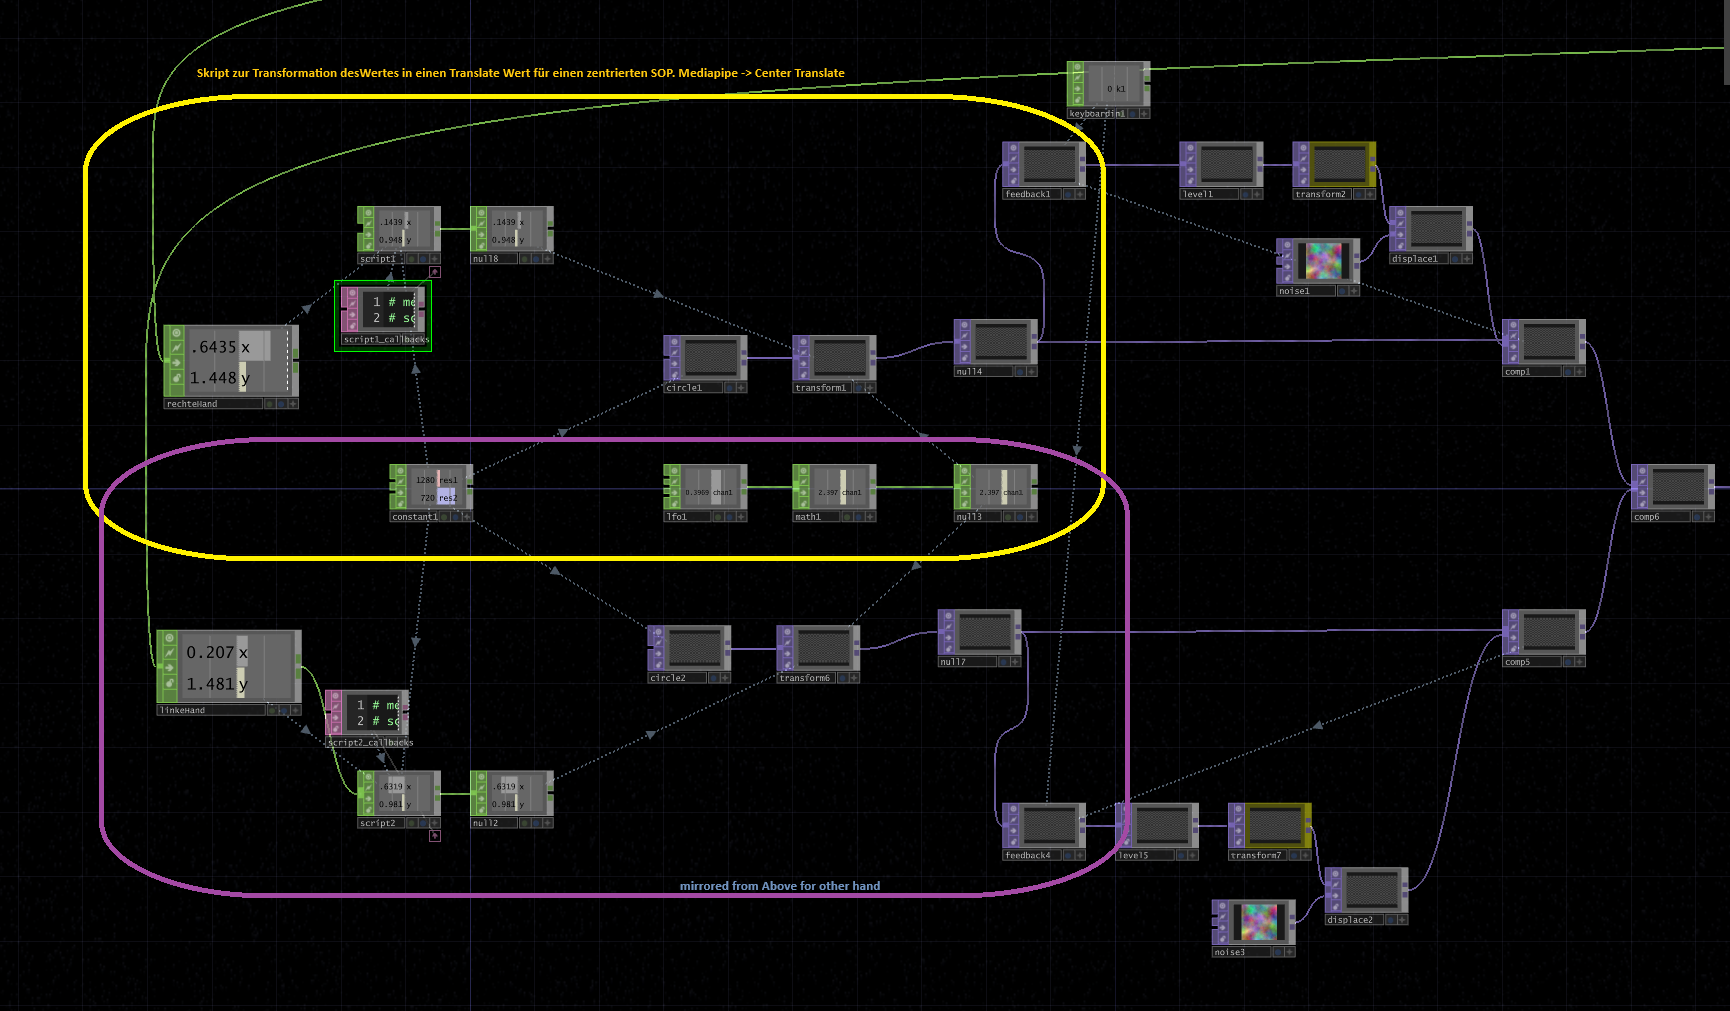
\includegraphics[width=0.6\textwidth,height=0.25\textheight,keepaspectratio]{images/docupictures/NodeXYzuSOPZentriertemTranslate.png}
%     \caption{Koordinatentransformation: MediaPipe-Normalisierung zu TouchDesigner-Weltkoordinaten}
%     \label{fig:coordinate_transform}
% \end{figure}

% DUPLICATE IMAGE - COMMENTED OUT
% \begin{figure}[!htbp]
%     \centering
%     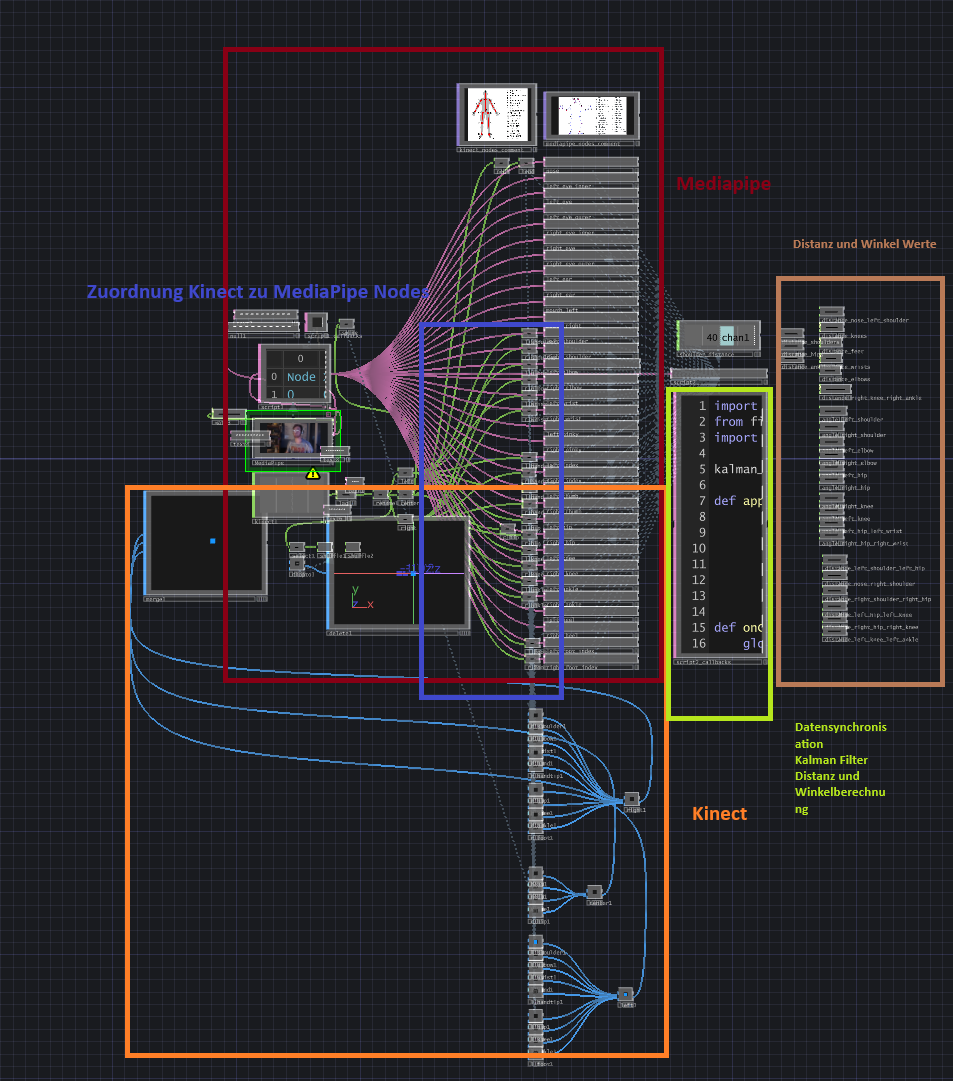
\includegraphics[width=0.6\textwidth,height=0.25\textheight,keepaspectratio]{images/docupictures/KinectMediaPipe_Testing.png}
%     \caption{Kinect-MediaPipe Geometrische Analyse: Echtzeit-Berechnung von Skelett-Relationen}
%     \label{fig:distance_angle}
% \end{figure}

% Ausfuehrungsdokumentation figures
% PLACEMENT: Ausfuehrungsdokumentation.tex - Production environment setup
\begin{figure}[!htbp]
   \centering
   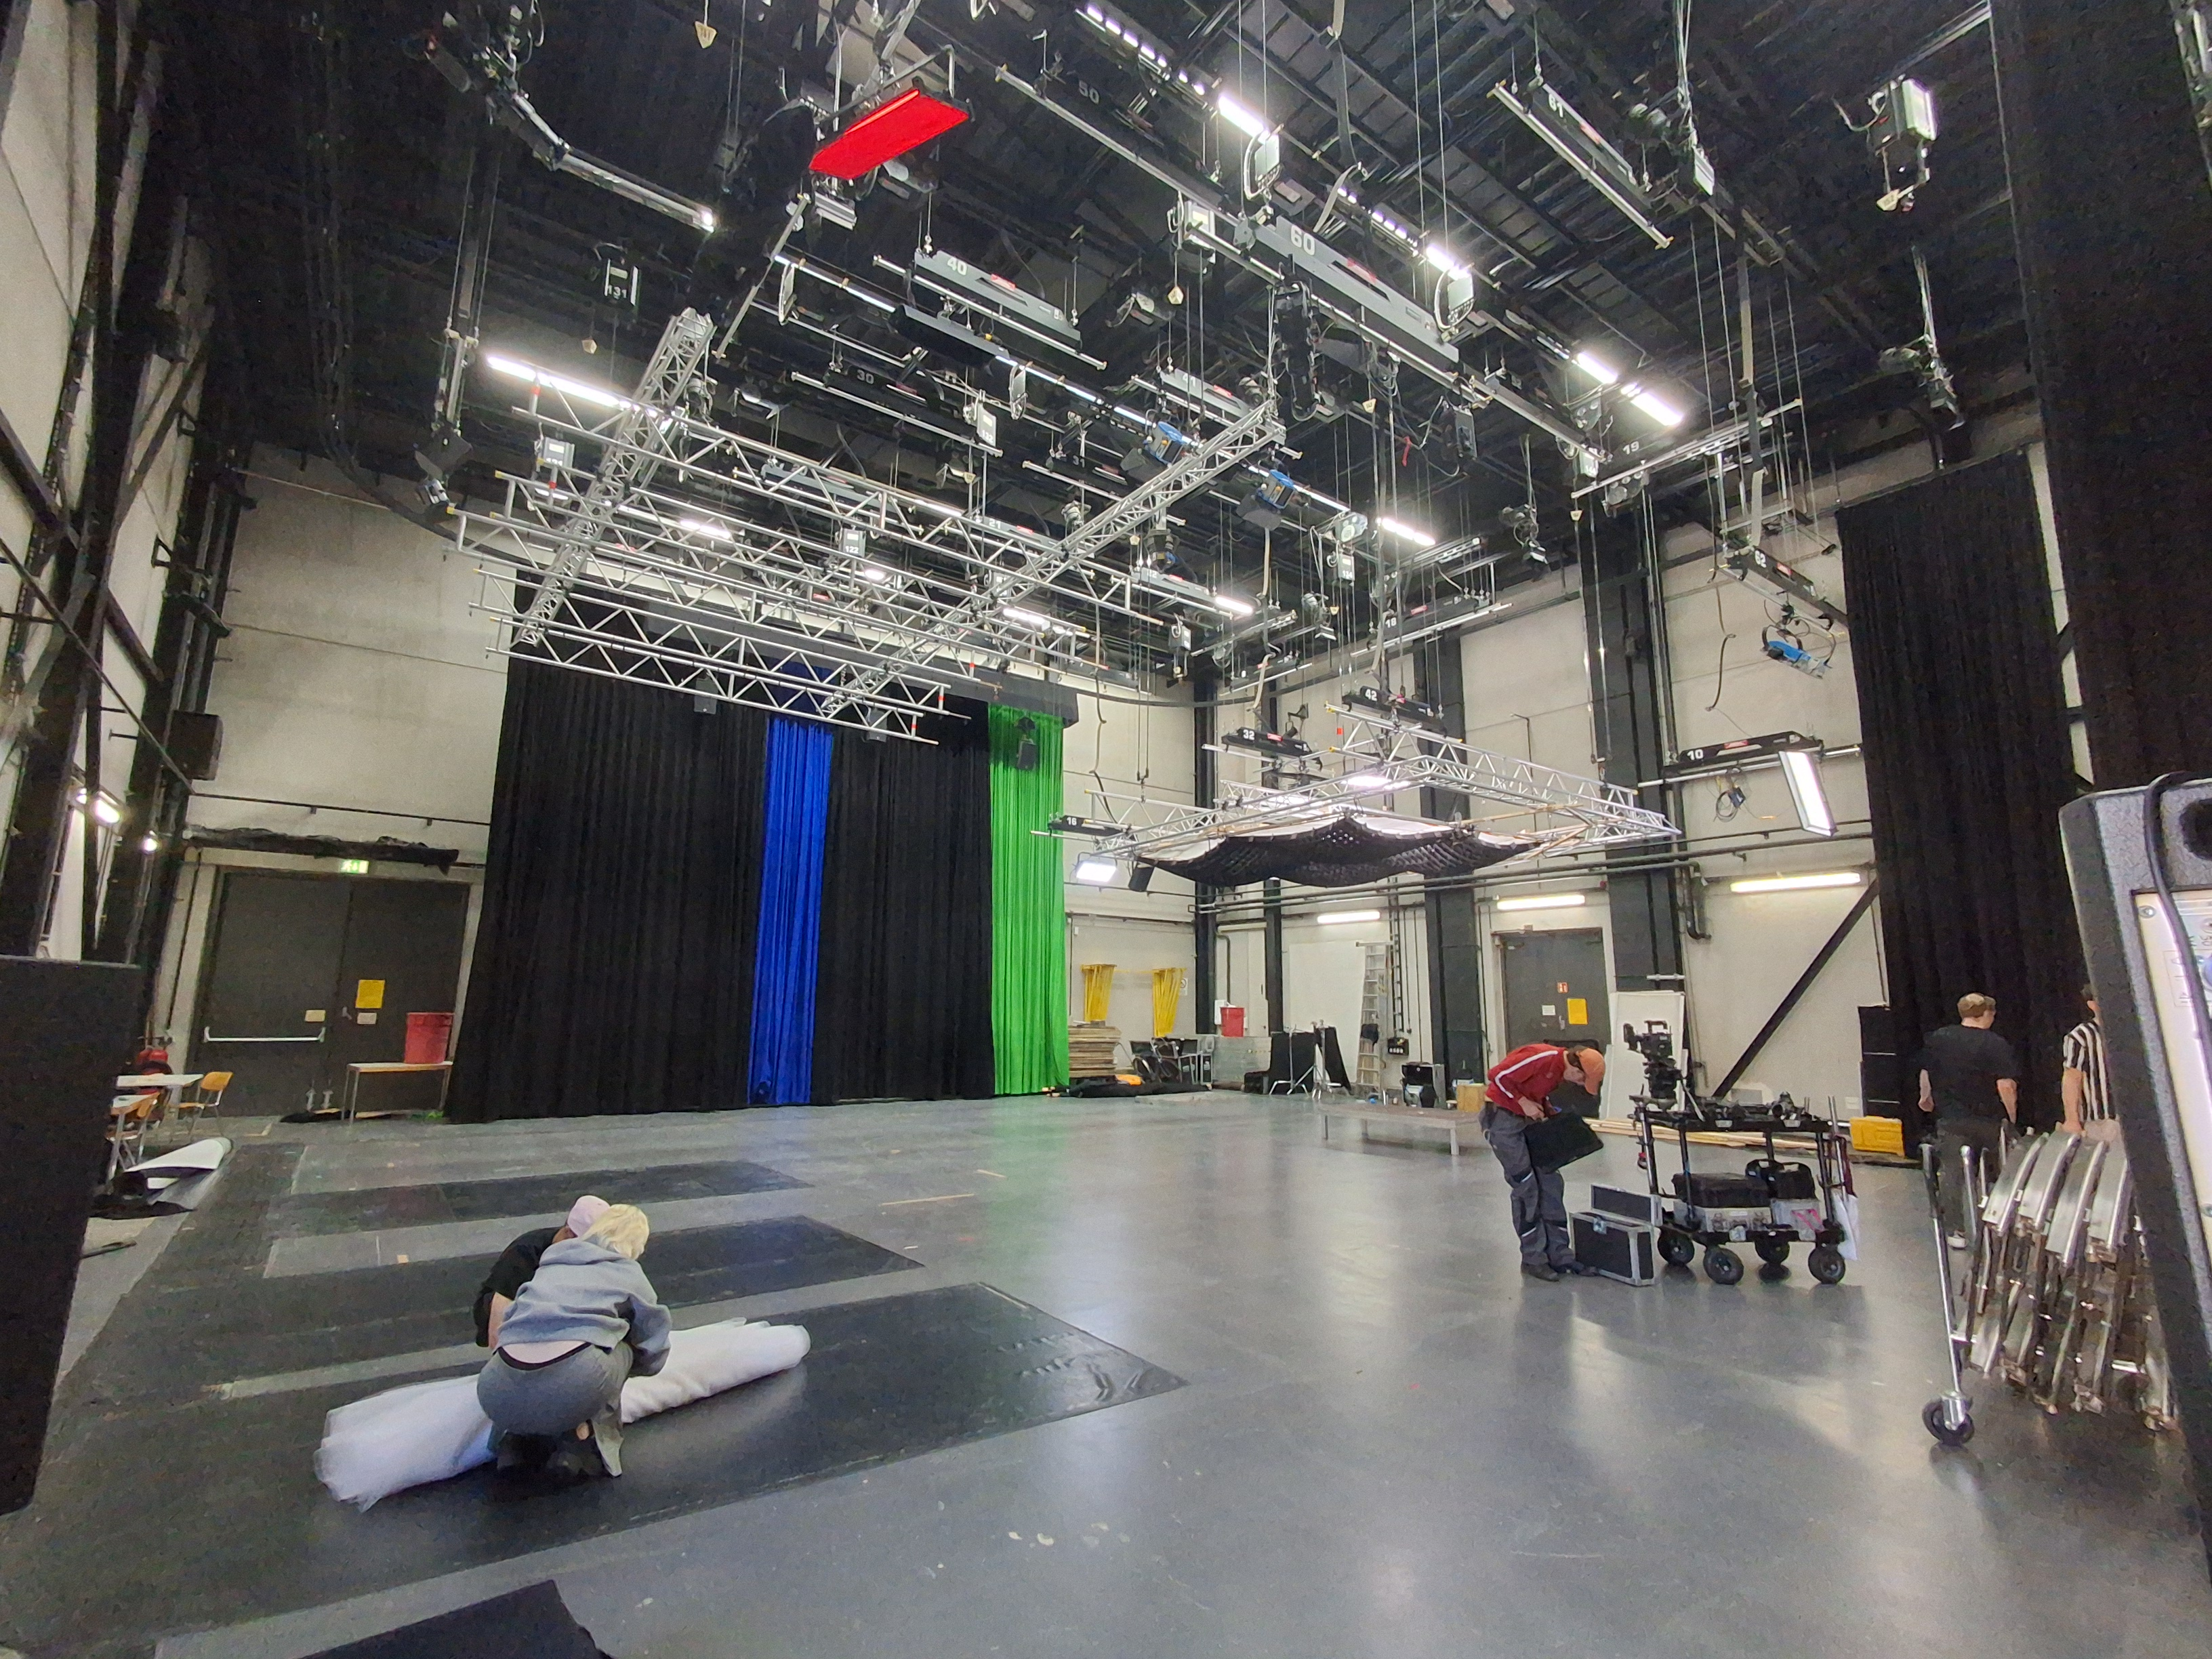
\includegraphics[width=0.6\textwidth,height=0.25\textheight,keepaspectratio]{images/onSetImages/InsideWideshotAlbrechtAdeStudio.jpg}
   \caption{Albrecht-Ade-Studio: Erste Eindr�cke der gro�en Soundstage vor Produktionsbeginn}
   \label{fig:studio_interior}
\end{figure}

% PLACEMENT: Ausfuehrungsdokumentation.tex - Technical operation during production
\begin{figure}[!htbp]
   \centering
   \includegraphics[width=0.6\textwidth,height=0.25\textheight,keepaspectratio]{images/onSetImages/MartyBehindTheStudioCurtainDoingTouchDesigner.jpg}
   \caption{Technische Umsetzung: TouchDesigner-Bedienung hinter dem Studievorhang w�hrend der Produktion}
   \label{fig:technical_operation}
\end{figure}

% PLACEMENT: Ausfuehrungsdokumentation.tex - Production preparation and setup
\begin{figure}[!htbp]
   \centering
   \includegraphics[width=0.6\textwidth,height=0.25\textheight,keepaspectratio]{images/onSetImages/wideStudioShotPreparingTopDownSpikeShot.jpg}
   \caption{Studio-Vorbereitung: Setup f�r Top-Down-Spike-System mit Overhead-Kamera-Positionierung}
   \label{fig:topdown_setup}
\end{figure}

% PLACEMENT: Ausfuehrungsdokumentation.tex - Production monitoring and results
\begin{figure}[!htbp]
   \centering
   \includegraphics[width=0.6\textwidth,height=0.25\textheight,keepaspectratio]{images/onSetImages/cameraBTSPicofACameraScreenOfTopDown64SpikeOfDancerOnFloor.jpg}
   \caption{Kameramonitor: Top-Down-Aufnahme des 64-Spike-Systems mit T�nzer auf dem Studioboden}
   \label{fig:camera_monitor}
\end{figure}

% PLACEMENT: Ausfuehrungsdokumentation.tex or ergebnisuebersicht.tex - Live system operation
\begin{figure}[!htbp]
   \centering
   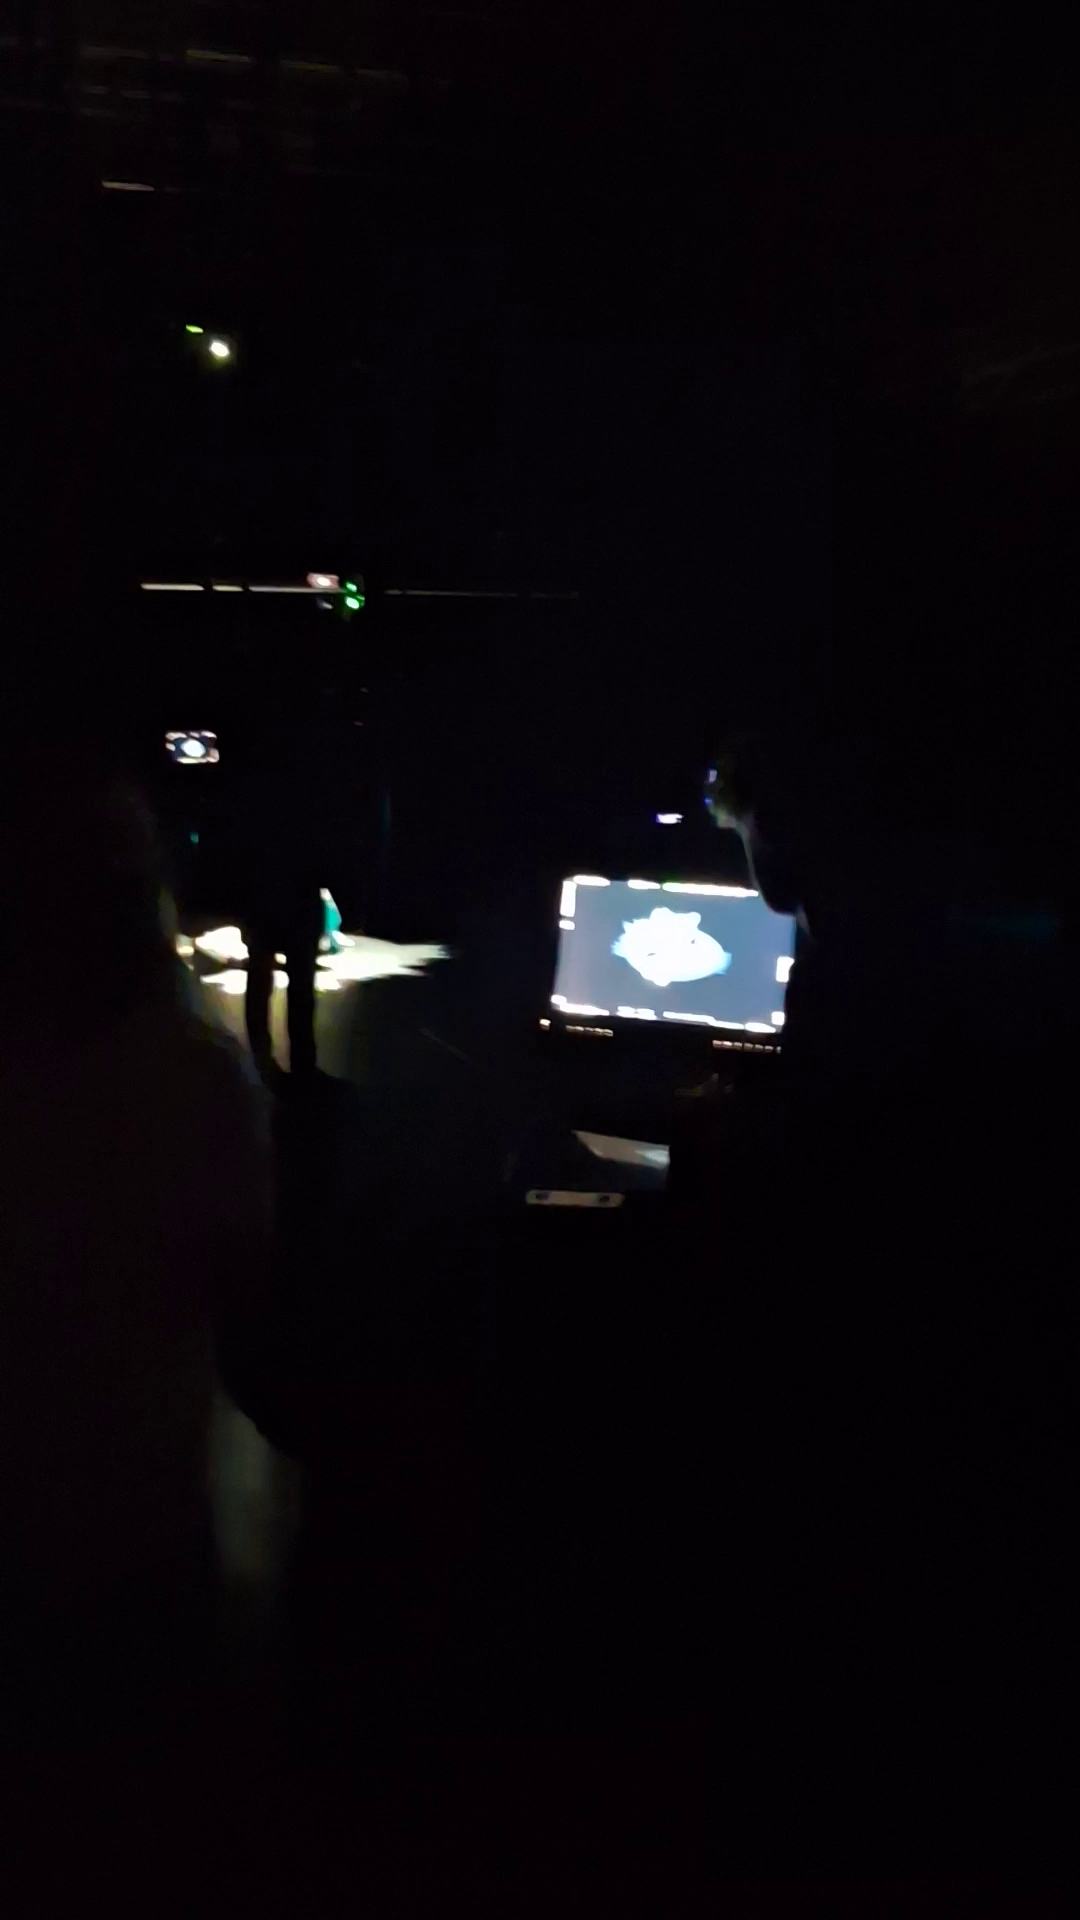
\includegraphics[width=0.6\textwidth,height=0.25\textheight,keepaspectratio]{images/BTS_ProducerScreen.png}
   \caption{Spike-System in Aktion: Reagiert pr�zise auf Hand- und Fu�bewegungen}
   \label{fig:spike_action}
\end{figure}

% PLACEMENT: Demonstration.tex or ergebnisuebersicht.tex - Head-tracking setup demonstration
\begin{figure}[!htbp]
   \centering
   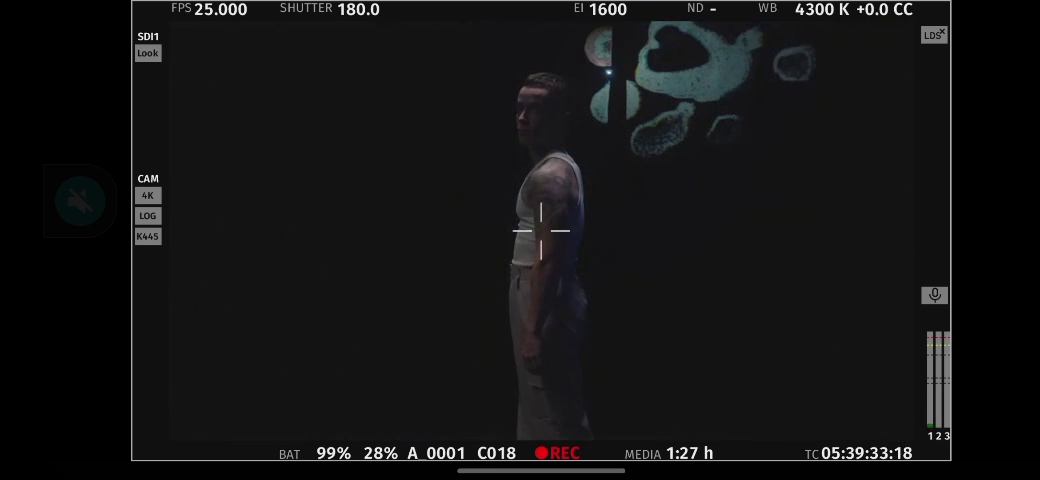
\includegraphics[width=0.6\textwidth,height=0.25\textheight,keepaspectratio]{images/HeadTracking_HQCamera.png}
   \caption{Kopfpartikel-Setup: Komplexe Kamera-Beamer-Ausrichtung}
   \label{fig:head_setup}
\end{figure}

% PLACEMENT: Ausfuehrungsdokumentation.tex - Production setup challenges
\begin{figure}[!htbp]
   \centering
   \includegraphics[width=0.6\textwidth,height=0.25\textheight,keepaspectratio]{images/onSetImages/PictureOfDancerBTSinSetupForHeadTrackingBubbles.jpg}
   \caption{Kopfpartikel-Setup: T�nzer bei Vorbereitung f�r Head-Tracking mit kritischen Lichtbedingungen}
   \label{fig:dancer_head_tracking}
\end{figure}

% PLACEMENT: Demonstration.tex or ergebnisuebersicht.tex - Head-tracking accuracy results
\begin{figure}[!htbp]
   \centering
   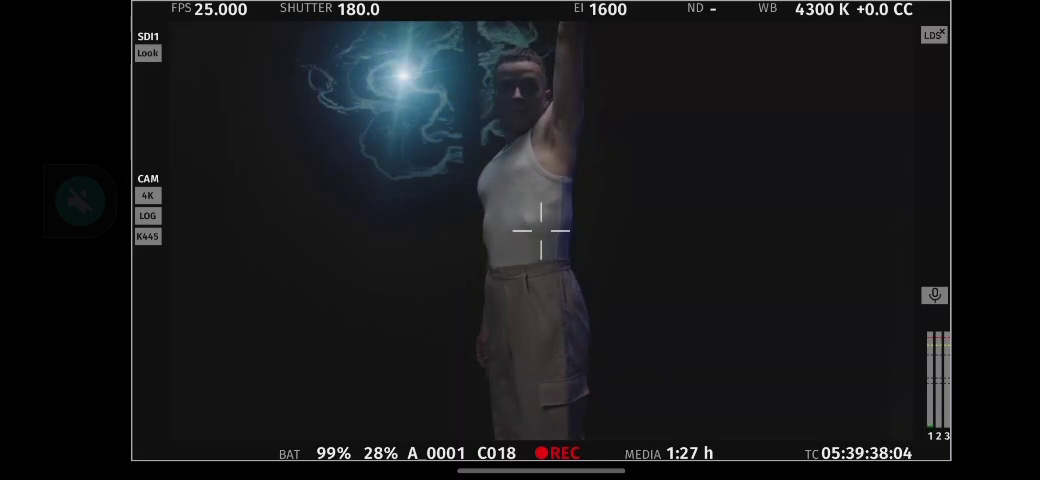
\includegraphics[width=0.6\textwidth,height=0.25\textheight,keepaspectratio]{images/HeadTrackingLeftSideOfHeadWithHeadClearlyAttached.png}
   \caption{Head-Tracking Perspektive: MediaPipe-Skelett-Erkennung aus seitlichem Blickwinkel}
   \label{fig:low_light_tracking}
\end{figure}

% PLACEMENT: Demonstration.tex or ergebnisuebersicht.tex - Successful head-tracking results
\begin{figure}[!htbp]
   \centering
   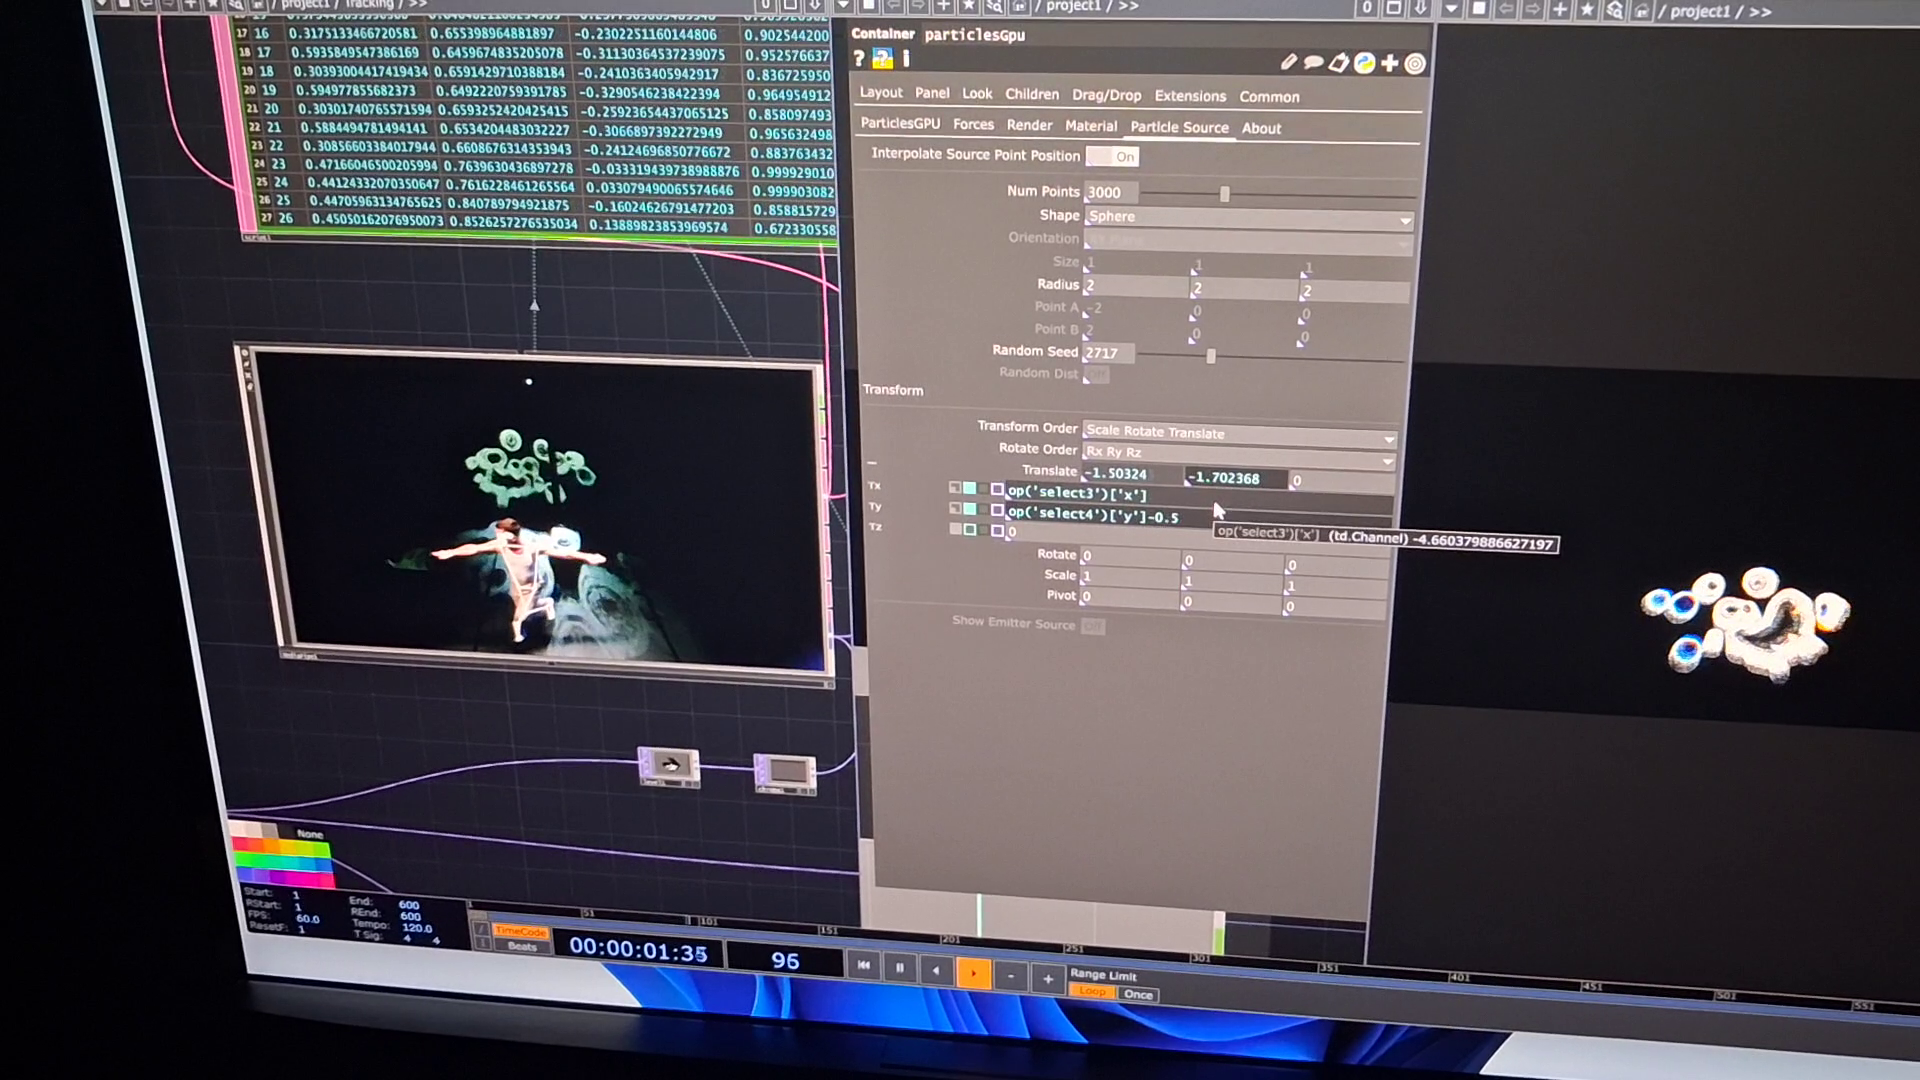
\includegraphics[width=0.6\textwidth,height=0.25\textheight,keepaspectratio]{images/HeadtrackingBubblesClearlyAtHeadLevelOnBackgroundBeamerMediaPipeSkeletonBeautifullyVisible.png}
   \caption{Head-Tracking-Bubbles Endergebnis: MediaPipe-Skelett-Erkennung mit Beamer-Projektion trotz Herausforderungen erfolgreich}
   \label{fig:head_result}
\end{figure}

% PLACEMENT: Demonstration.tex or ergebnisuebersicht.tex - Hand-fire effect demonstration
\begin{figure}[!htbp]
   \centering
   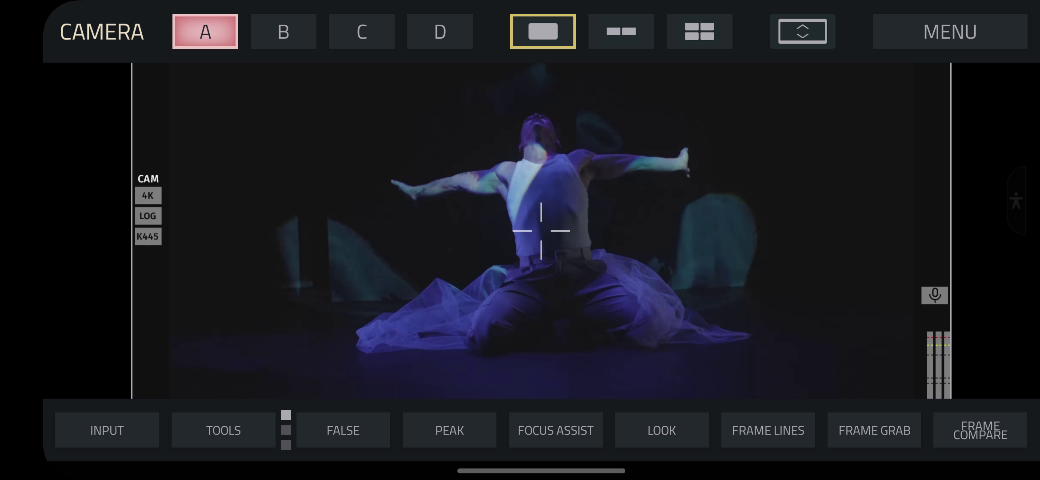
\includegraphics[width=0.6\textwidth,height=0.25\textheight,keepaspectratio]{images/HQCinemaCameraPerspectiveOfHandFireToTheSidesOfTheHands.png}
   \caption{Hand-Feuer Setup: Modulare Architektur bew�hrt sich}
   \label{fig:hand_fire_setup}
\end{figure}

% PLACEMENT: erkenntnisse.tex or nutzererfahrung.tex - System limitations and challenges
\begin{figure}[!htbp]
   \centering
   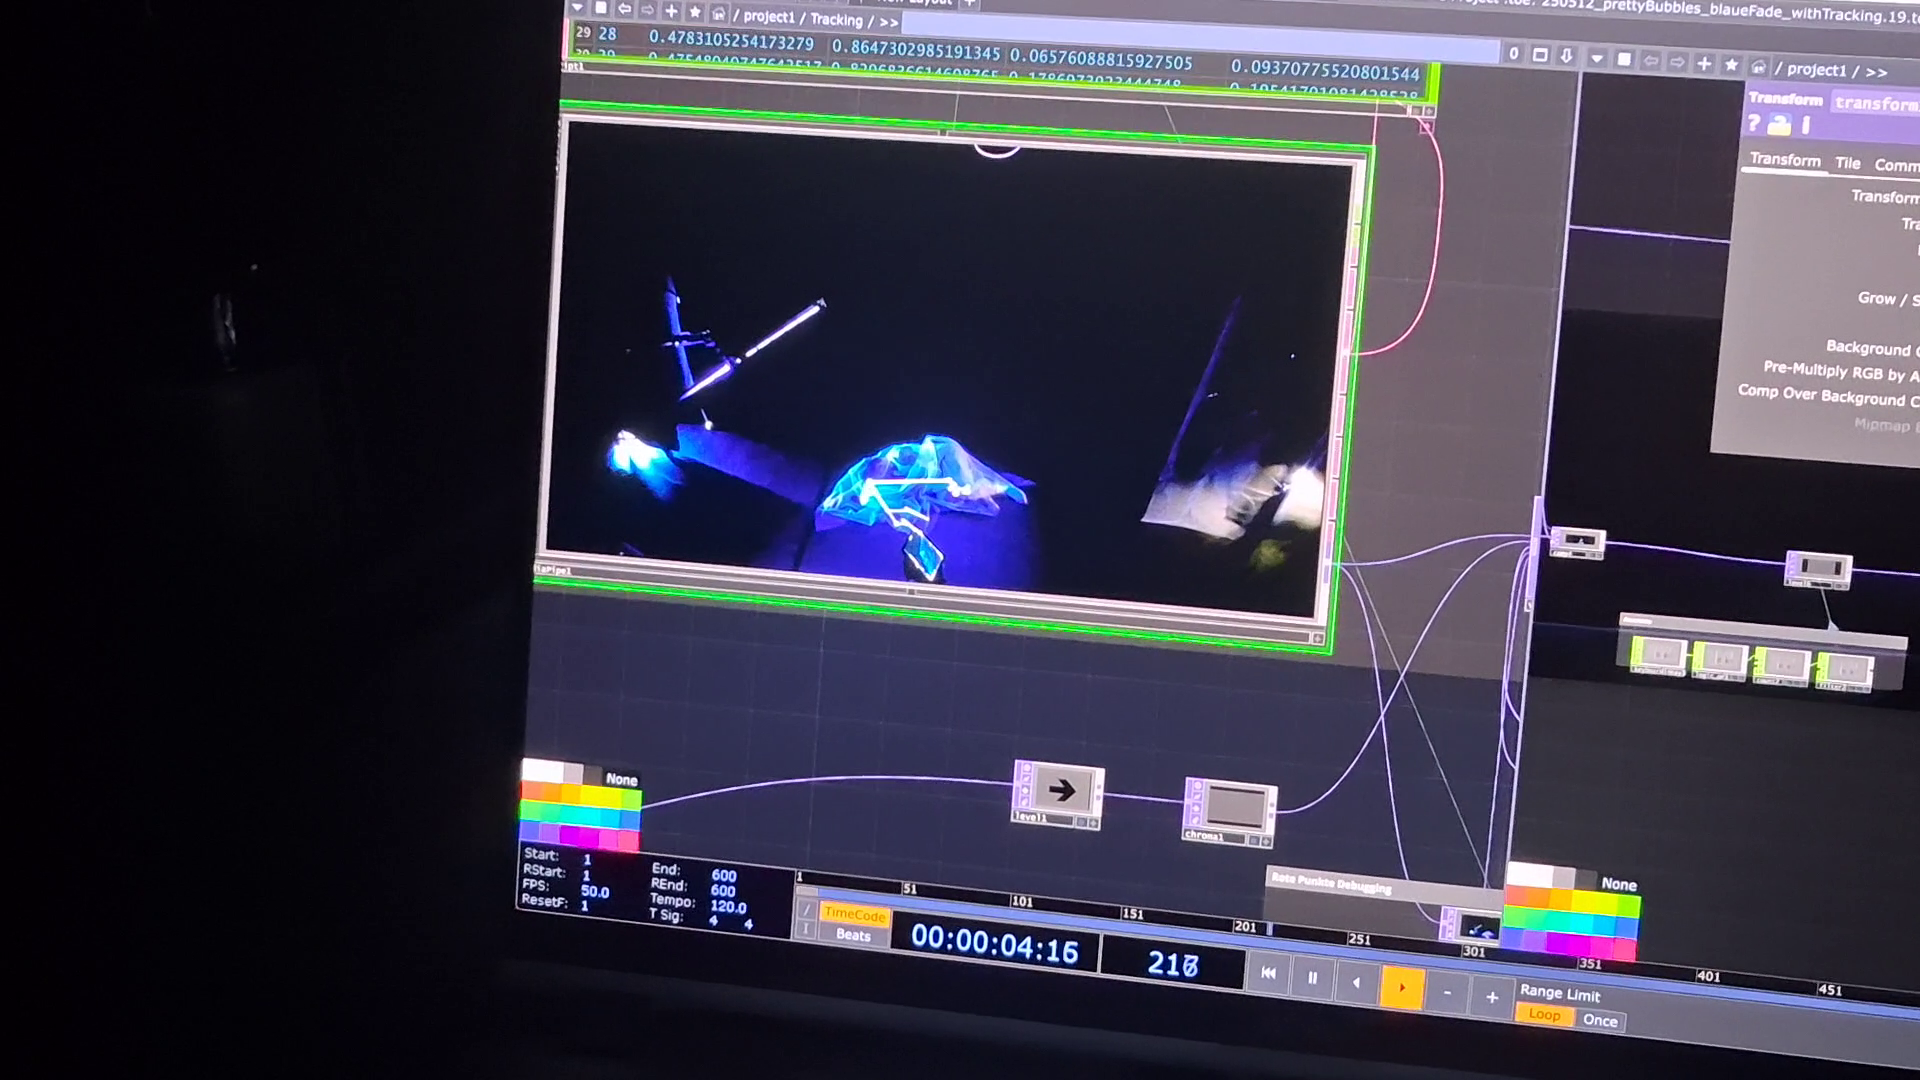
\includegraphics[width=0.6\textwidth,height=0.25\textheight,keepaspectratio]{images/DancerNotMediaPipeFoundCorrectlyWhenInClothOnFloor.png}
   \caption{Tracking-Problem: MediaPipe verliert Tänzer-Skelett-Erkennung bei Stoffverschleierung}
   \label{fig:cloth_tracking_issue}
\end{figure}

% PLACEMENT: Demonstration.tex or ergebnisuebersicht.tex - Live effect demonstration
\begin{figure}[!htbp]
   \centering
   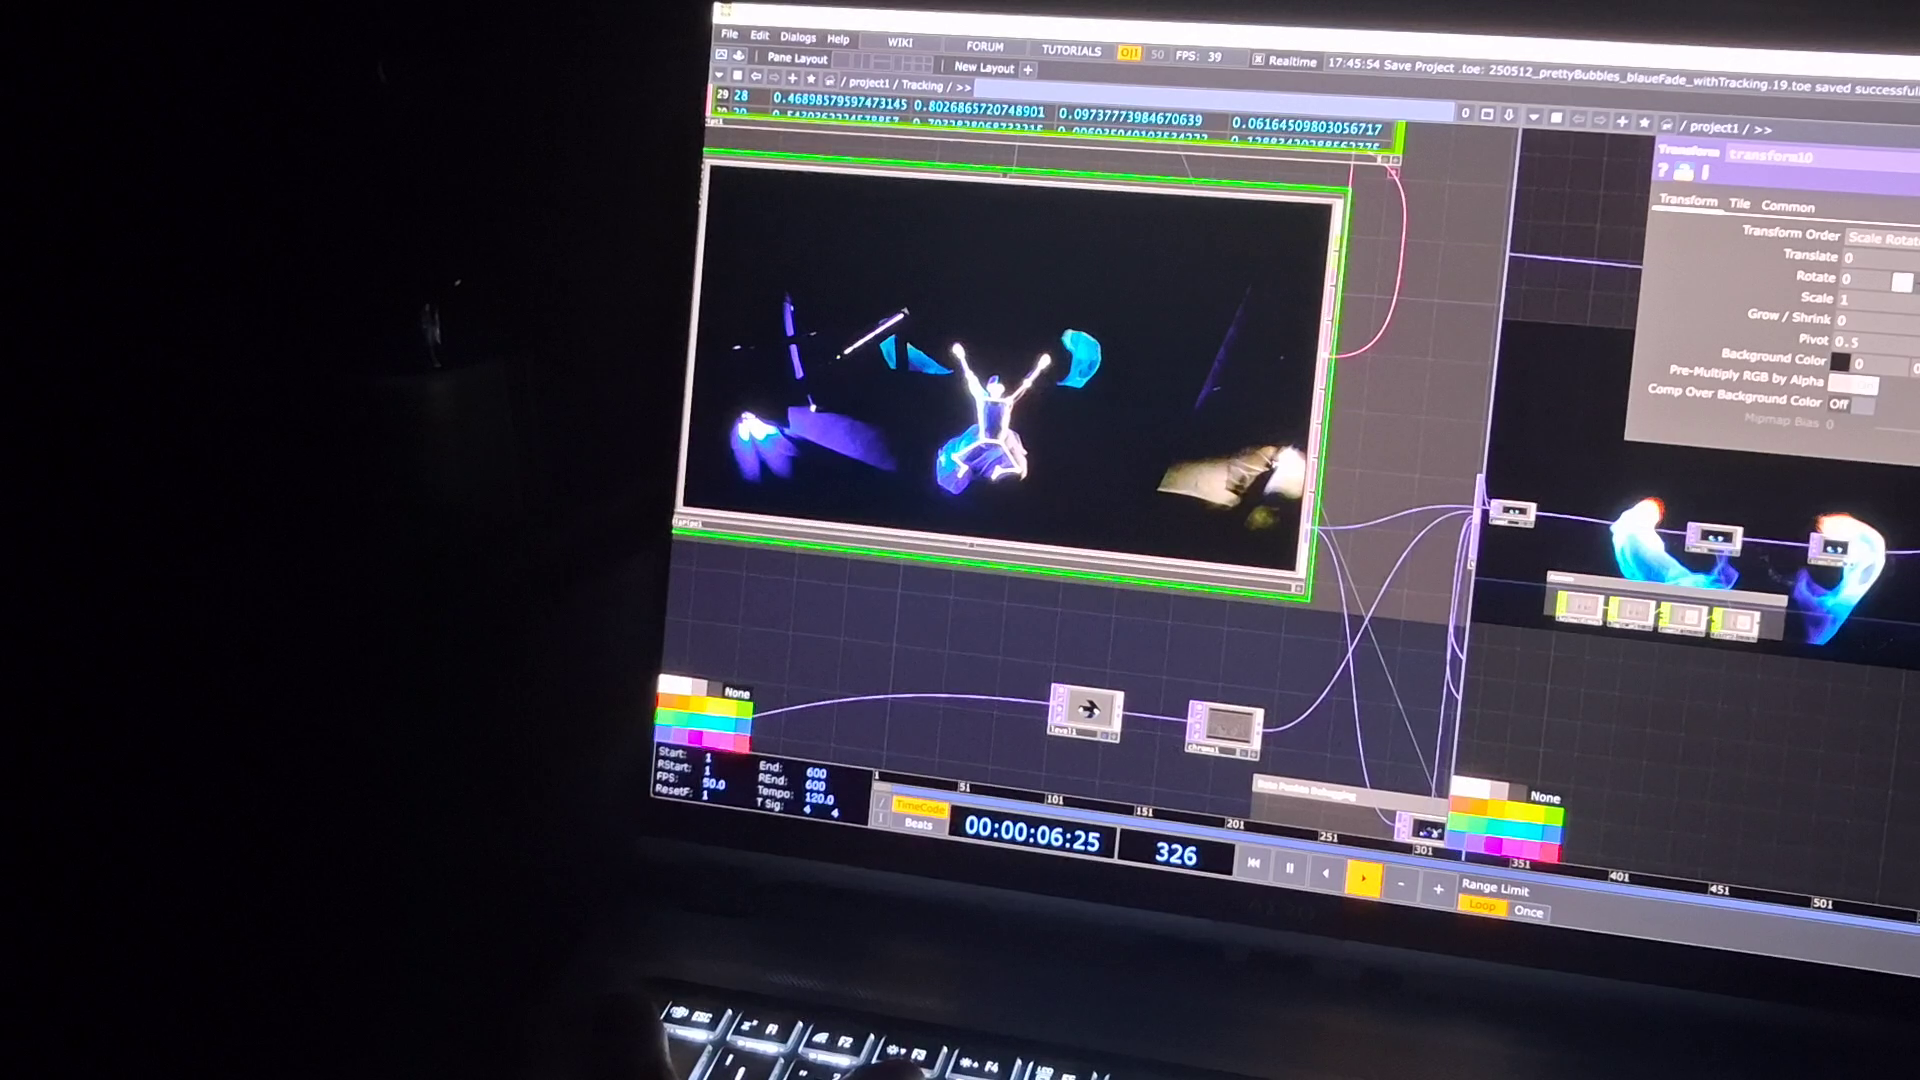
\includegraphics[width=0.6\textwidth,height=0.25\textheight,keepaspectratio]{images/dancerWithHandFireViewFromKinect.png}
   \caption{Hand-Feuer in Aktion: Blaue Partikel folgen den H�nden}
   \label{fig:hand_fire_action}
\end{figure}

% PLACEMENT: Ausfuehrungsdokumentation.tex - Production conclusion
\begin{figure}[!htbp]
   \centering
   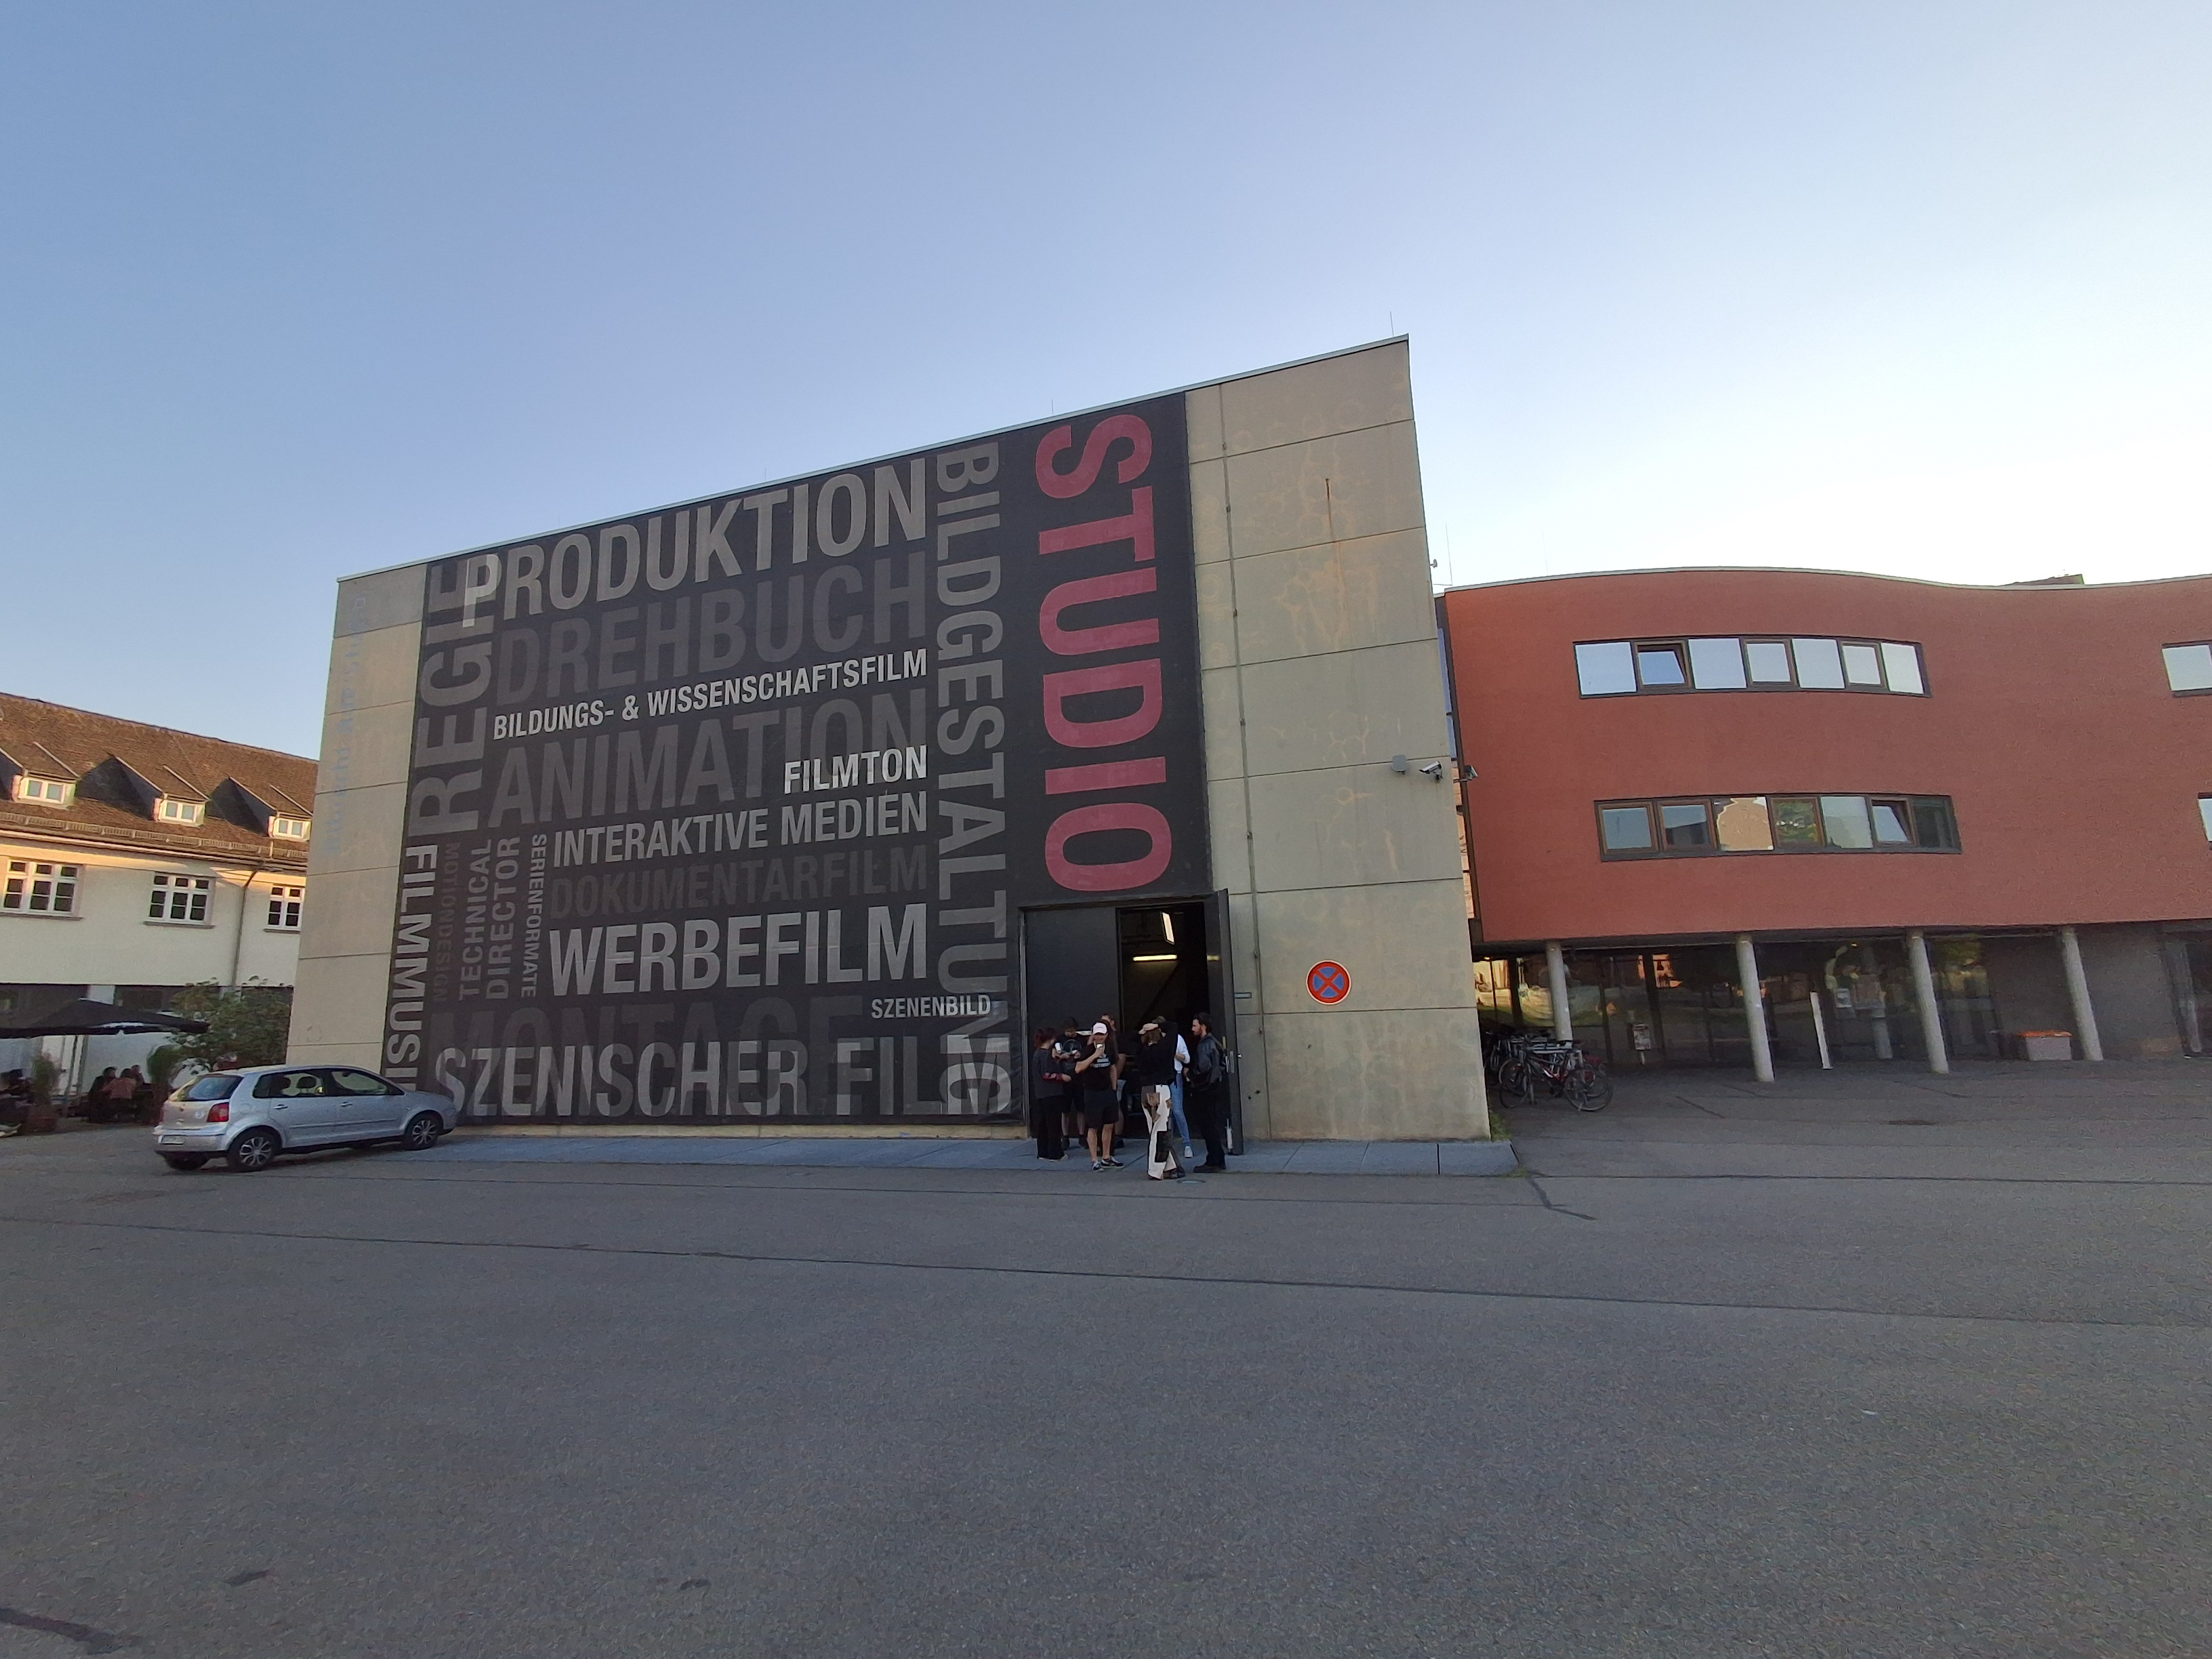
\includegraphics[width=0.6\textwidth,height=0.25\textheight,keepaspectratio]{images/onSetImages/WideShotOfOutsideOfStudioAfter2DayShoot.jpg}
   \caption{Produktionsabschluss: Au�enansicht des Albrecht-Ade-Studios nach zweit�giger Drehzeit}
   \label{fig:studio_exterior}
\end{figure}

% DUPLICATE IMAGE - COMMENTED OUT
% \begin{figure}[!htbp]
%    \centering
%    \includegraphics[width=0.6\textwidth,height=0.25\textheight,keepaspectratio]{images/onSetImages/wideStudioShotPreparingTopDownSpikeShot.jpg}
%    \caption{Behind-the-Scenes Top-Down-Setup: Professionelle Crew integriert M.A.S.K. Spike-System in den Workflow}
%    \label{fig:crew_setup}
% \end{figure}

% PLACEMENT: Ausfuehrungsdokumentation.tex - Team dynamics and production atmosphere
\begin{figure}[!htbp]
   \centering
   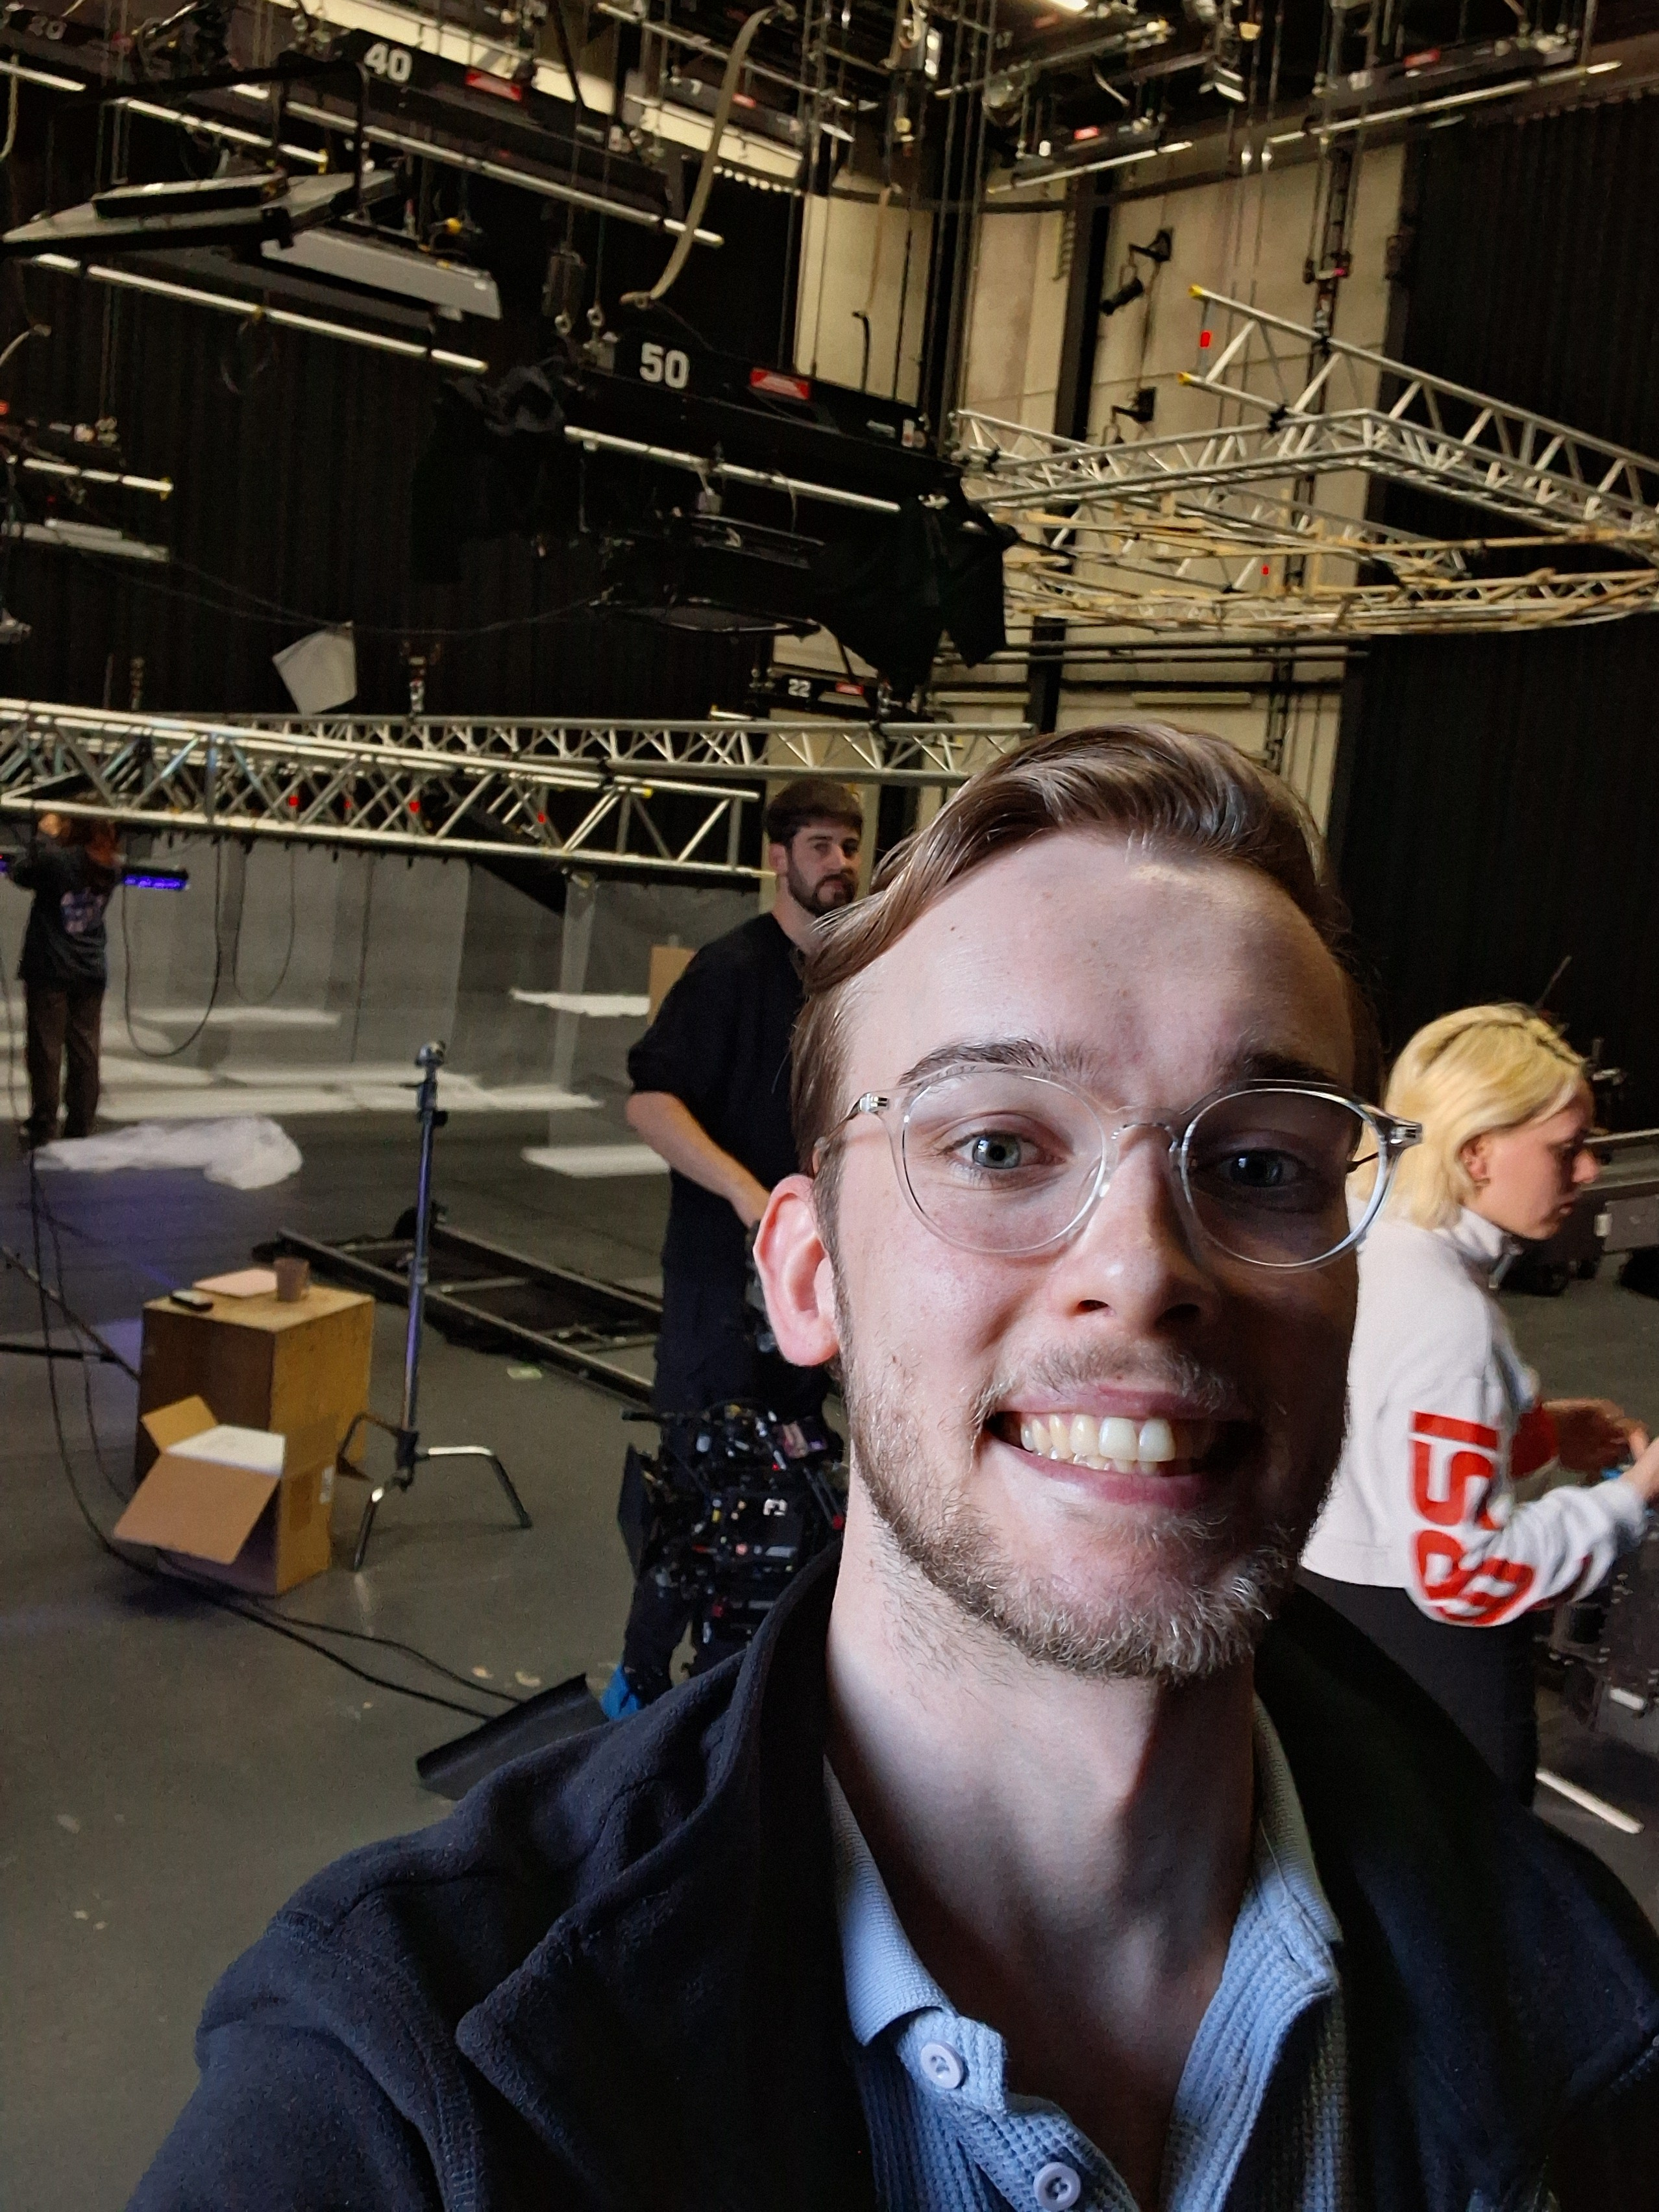
\includegraphics[width=0.6\textwidth,height=0.25\textheight,keepaspectratio]{images/onSetImages/MartySmileyIntoCameraOnSet.jpg}
   \caption{Teamdynamik: Entspannte Atmosph�re zwischen den Takes trotz technischer Herausforderungen}
   \label{fig:team_atmosphere}
\end{figure}

% PLACEMENT: Ausfuehrungsdokumentation.tex - Production workflow and setup
\begin{figure}[!htbp]
   \centering
   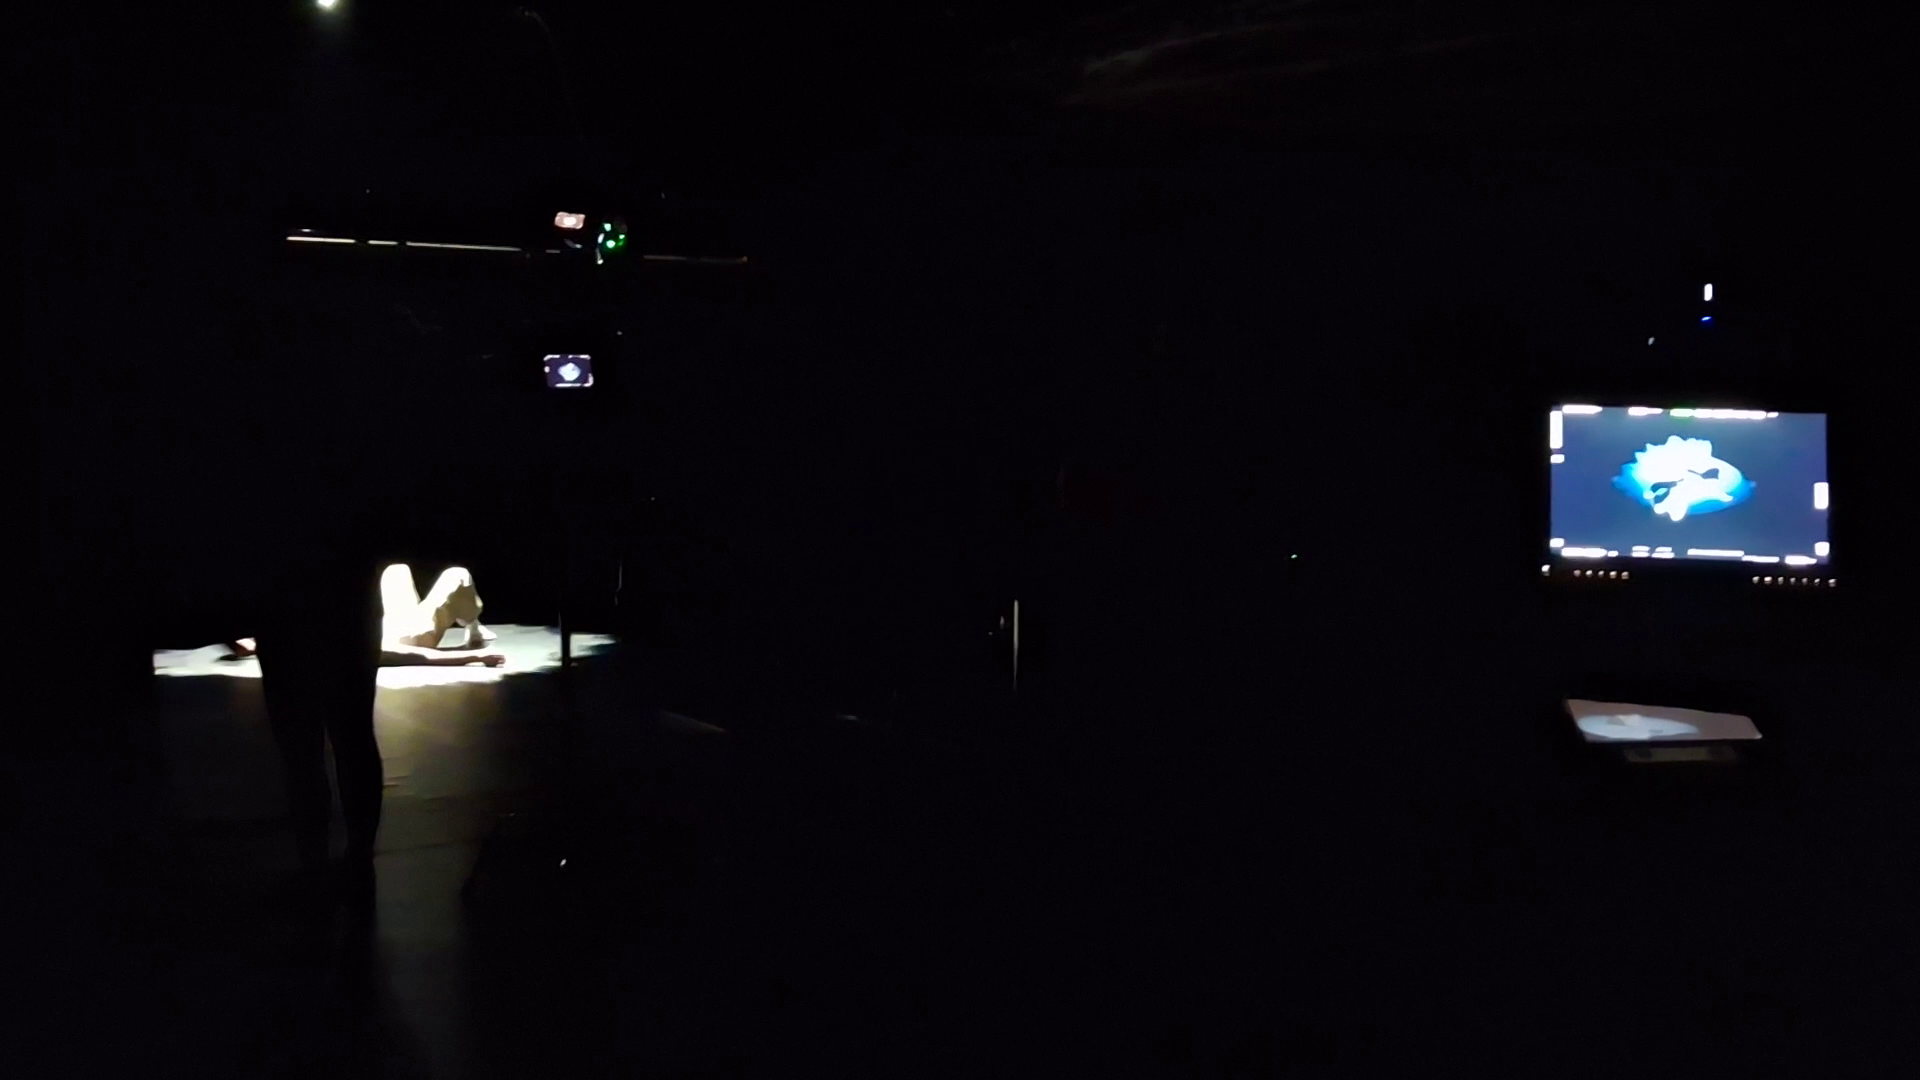
\includegraphics[width=0.6\textwidth,height=0.25\textheight,keepaspectratio]{images/BTS_TopDown_DancerAndProducer.png}
   \caption{Behind the Scenes: T�nzer mit professioneller Lichttechnik und Producer-Ansicht}
   \label{fig:studio_wide}
\end{figure}

% Generierte LaTeX-Figure-Einträge für ungenutzte PNG-Bilder
% Diese Abbildungen dokumentieren wichtige Aspekte des M.A.S.K.-Systems
% Fügen Sie diese an passenden Stellen in images.tex ein

% ===== Behind-the-Scenes Produktionsdokumentation =====
% Für Abschnitt: Ausführungsdokumentation

% PLACEMENT: Ausfuehrungsdokumentation.tex - Live production monitoring
\begin{figure}[htbp]
    \centering
    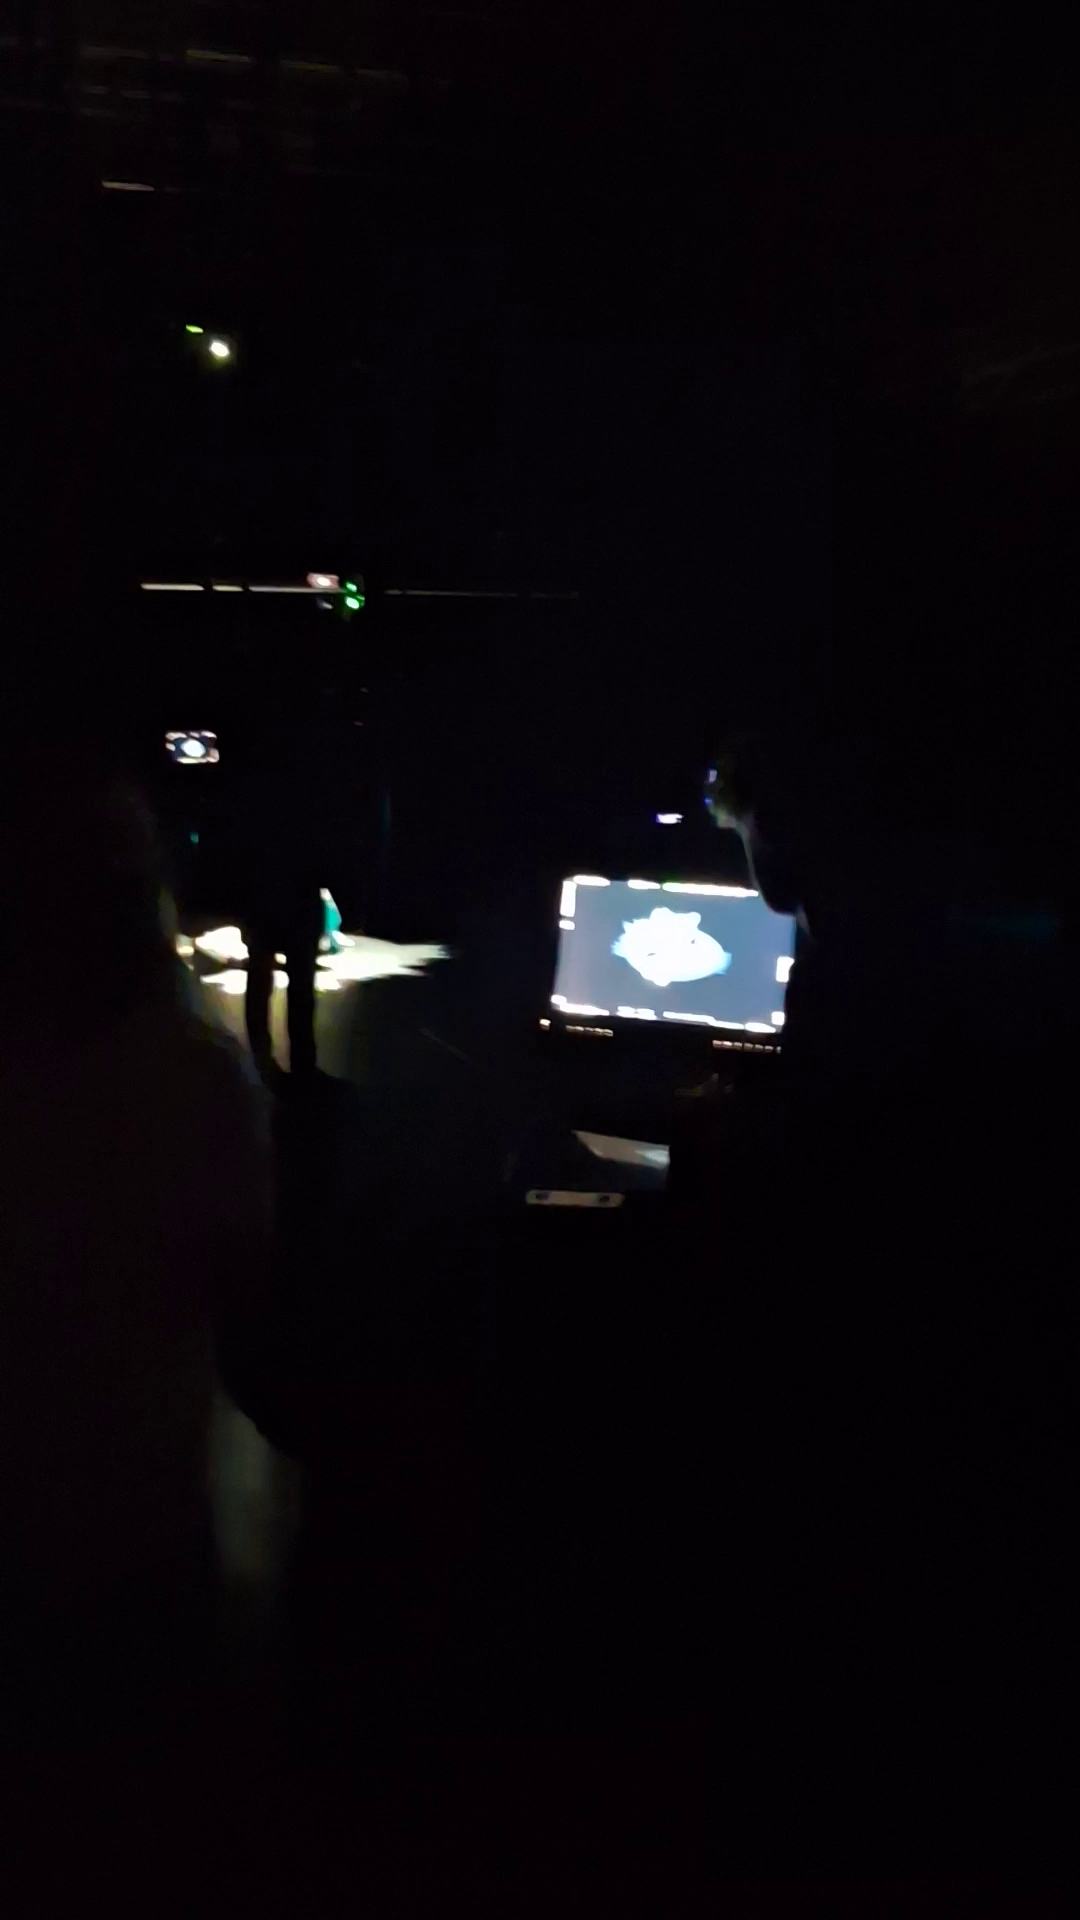
\includegraphics[width=0.8\textwidth,height=0.4\textheight,keepaspectratio]{images/BehindTheScenesDuringShotTopDownProducerScreenVisibleAsWellAsDancerOnFloor.png}
    \caption{Behind-the-Scenes: Producer-Monitor zeigt 64-Spike-Visualisierung während Tänzer auf dem Studioboden performt}
    \label{fig:bts_topdown_produktion}
\end{figure}

% PLACEMENT: Ausfuehrungsdokumentation.tex - Production setup and lighting
\begin{figure}[htbp]
    \centering
    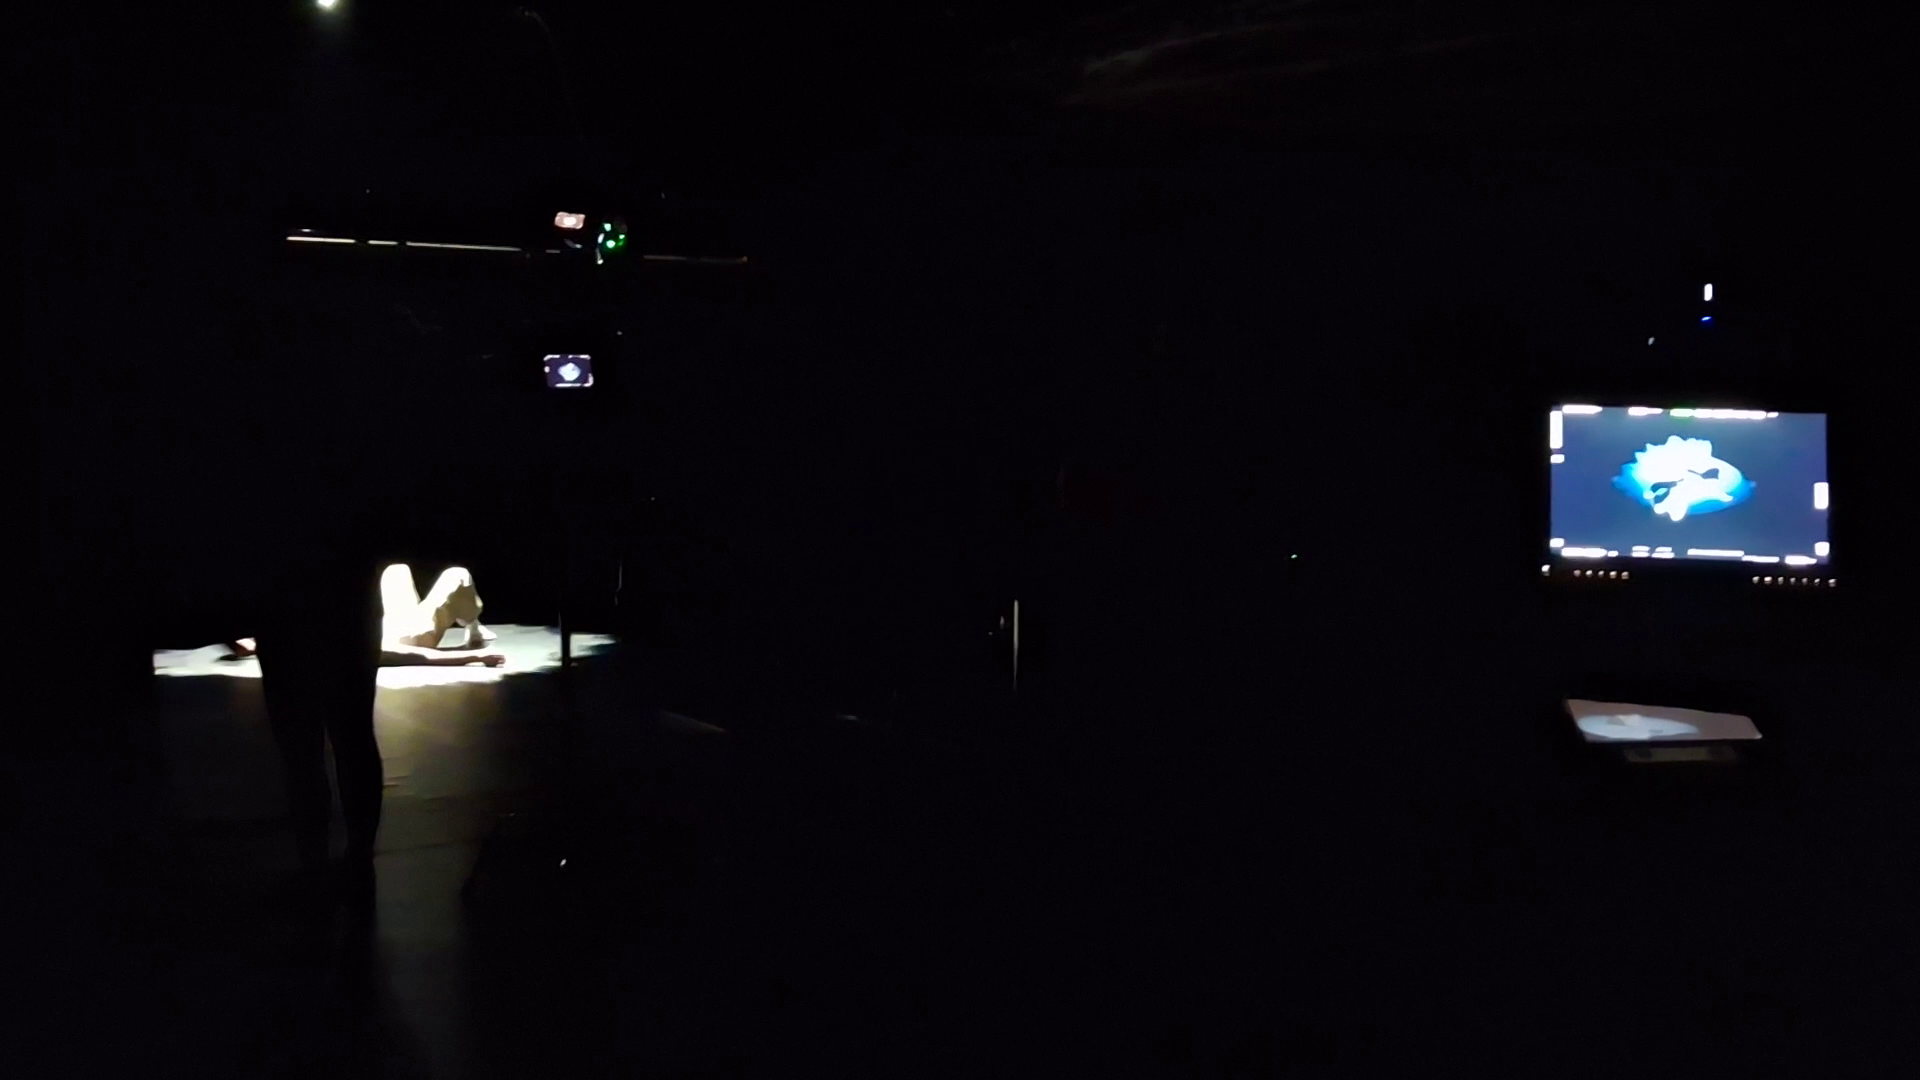
\includegraphics[width=0.8\textwidth,height=0.4\textheight,keepaspectratio]{images/BehindTheScenesTopDownWithDancerOnTheLeftInsideTheHeavyLightAndProducerViewOnRightSide.png}
    \caption{Produktionsaufbau: Tänzer unter professioneller Studiobeleuchtung (links) und TouchDesigner-Steuerungsinterface des Producers (rechts)}
    \label{fig:bts_topdown_splitview}
\end{figure}

% ===== Visual-Effekt-Demonstrationen =====
% Für Abschnitt: Demonstration oder Systemarchitektur

% PLACEMENT: Demonstration.tex or ergebnisuebersicht.tex - Key visual effect demonstration
\begin{figure}[htbp]
    \centering
    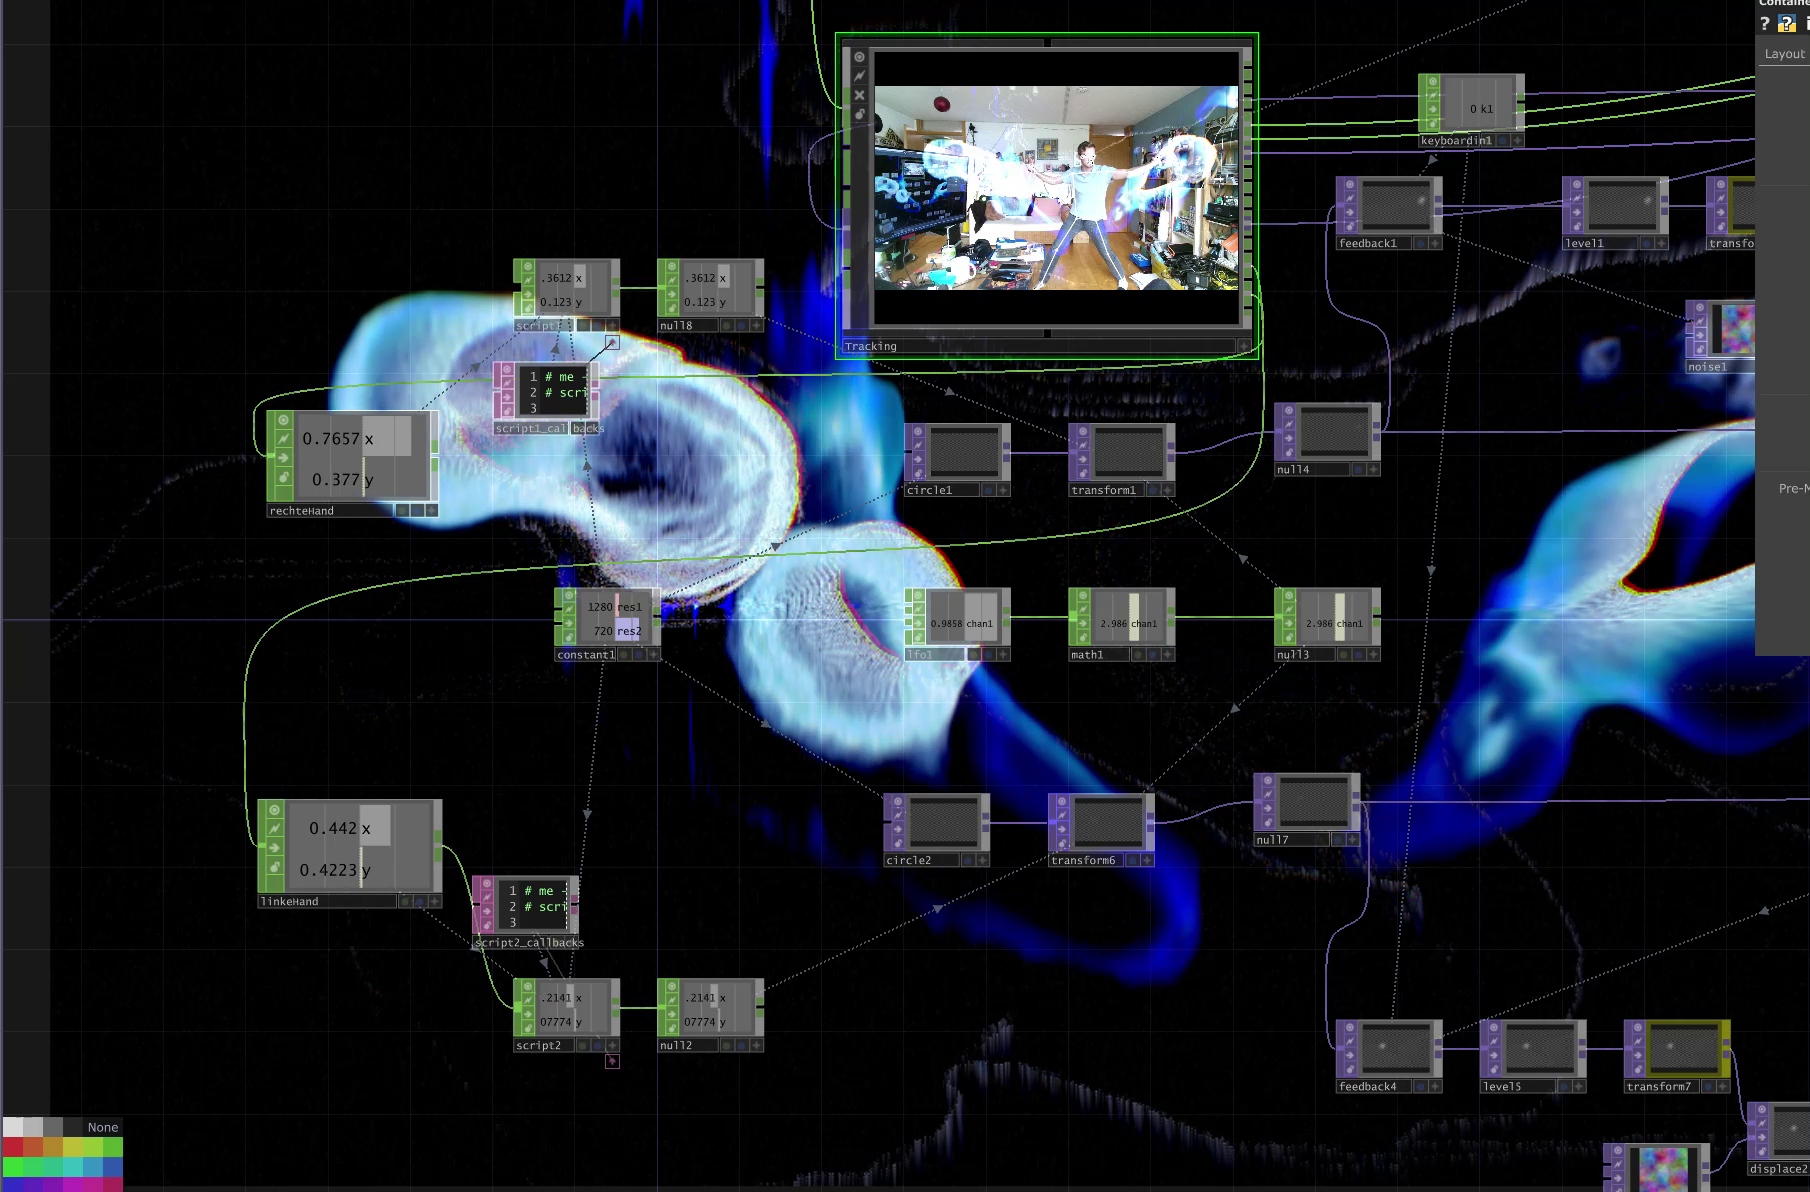
\includegraphics[width=0.8\textwidth,height=0.4\textheight,keepaspectratio]{images/DemonstrationOfTheMagicalFireHands.png}
    \caption{Live-Demonstration des NoisyBlob Hand-Feuer-Effekts: Blaue Partikel-Emission bei Handhebung über Hüfthöhe}
    \label{fig:handfeuer_demonstration}
\end{figure}

% ===== Head-Tracking-System Ansichten =====
% Für Abschnitt: Systemarchitektur oder Demonstration

% PLACEMENT: Demonstration.tex or Systemarchitektur_und_Ergebnisse.tex - Precise tracking demonstration
\begin{figure}[htbp]
    \centering
    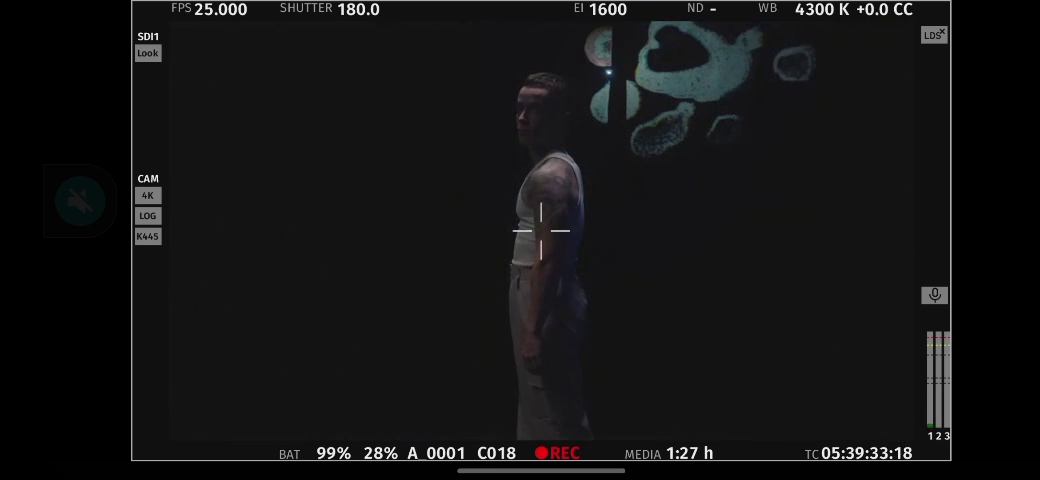
\includegraphics[width=0.8\textwidth,height=0.4\textheight,keepaspectratio]{images/HQCameraHeadtrackingVisibleWithBubblesOffsetCorrectlyFromHQCameraViewToAppearOnRightSideOfHead.png}
    \caption{HQ-Kameraperspektive: Kopfpartikel mit korrektem Offset zur rechten Seite des Performers für präzise Beamer-Projektion}
    \label{fig:headtracking_hq_kamera_offset}
\end{figure}

% PLACEMENT: Systemarchitektur_und_Ergebnisse.tex or anhang_technische_spezifikationen.tex - Technical debugging visualization
\begin{figure}[htbp]
    \centering
    \includegraphics[width=0.8\textwidth,height=0.4\textheight,keepaspectratio]{images/HeadTrackingPerspectiveTouchDesignerWithVisualsOverlayedAboveDebugCompToSeeaccurateTrackingOfParticleGPUaboveHeadWithReallifeBeamerProjectionCorrectlyPlaced.png}
    \caption{Debug-Visualisierung: Präzises ParticleGPU-Tracking über Kopfposition mit korrekt ausgerichteter Beamer-Projektion}
    \label{fig:headtracking_debug_overlay}
\end{figure}

% PLACEMENT: erkenntnisse.tex or Systemarchitektur_und_Ergebnisse.tex - Technical challenges and solutions
\begin{figure}[htbp]
    \centering
    \includegraphics[width=0.8\textwidth,height=0.4\textheight,keepaspectratio]{images/HeadTrackedBubblesInActionTouchDesignerPerspectiveslightMediaPipeFrameDelaySeeableButAlsoVisualsDirectlyAtHead.png}
    \caption{TouchDesigner Head-Tracking in Aktion: Kopfpartikel-Bubbles mit sichtbarer MediaPipe-Frame-Verzögerung aber direkter visueller Kopfanbindung}
    \label{fig:headtracking_bubbles_aktion}
\end{figure}

% ===== Technische Implementierung =====
% Für Abschnitt: Entwicklungsprozess oder Systemarchitektur

% PLACEMENT: Systemarchitektur_und_Ergebnisse.tex - Core technical solution for production environments
\begin{figure}[htbp]
    \centering
    \includegraphics[width=0.8\textwidth,height=0.4\textheight,keepaspectratio]{images/InfraRedOBSCameraToMediaPipeForTopDownCirlceGradeMapping.png}
    \caption{Infrarot-Pipeline: Kinect V2 IR-Stream über OBS Virtual Camera zu MediaPipe für störungsfreies Top-Down-Tracking}
    \label{fig:infrarot_topdown_mapping}
\end{figure}

% PLACEMENT: Systemarchitektur_und_Ergebnisse.tex or anhang_technische_spezifikationen.tex - Complete system architecture
\begin{figure}[htbp]
    \centering
    \includegraphics[width=0.8\textwidth,height=0.4\textheight,keepaspectratio]{images/docupictures/Finished_MediaPipeContainer.png}
    \caption{Vollständiger MediaPipe-Integration-Container: Modulare Node-Netzwerk-Architektur für Skelett-Tracking-Datenverarbeitung}
    \label{fig:mediapipe_container_komplett}
\end{figure}

% ===== ENCODING-FIX ERFORDERLICH =====
% In images.tex müssen ALLE Vorkommen von:
% 'Finished_MediaPipeContainer_mitErkl�rungen.png'
% ersetzt werden durch:
% 'Finished_MediaPipeContainer_mitErklärungen.png'
% Das Zeichen 'ä' wird fälschlicherweise als '�' enkodiert

% ===== AUSKOMMENTIERTE REFERENZEN =====
% Die folgenden PNG-Referenzen sind in images.tex auskommentiert:
% - Zeile 87: debug_visualization.png (Datei existiert nicht)
% - Zeile 168: infrared_pipeline_diagram.png (Datei existiert nicht)
% Erwägen Sie, diese Diagramme zu erstellen oder die auskommentierten Referenzen zu entfernen

% ===== HINWEISE ZUR VERWENDUNG =====
% 1. Diese Bilder sollten in die passenden Abschnitte eingefügt werden
% 2. Die Labels folgen dem Schema: fig:kategorie_beschreibung
% 3. Die Captions erklären den technischen Kontext gemäß der Dokumentation
% 4. Einige Bilder zeigen wichtige Behind-the-Scenes Momente der Produktion

